%%% MEMOIR CLASS %%%
\documentclass[twoside,12pt,openright,final,english]{memoir}
% Memoir Divisions: \book, \part, \chapter, \section, \subsection
% Fine divisions:   \subsubsection, \paragraph \subparagraph.
%%% END MEMOIR CLASS %%%

\setlength{\parskip}{\baselineskip}%
\setlength{\parindent}{0pt}%

\usepackage{float}

\usepackage{graphicx}
% For full size print graphics
\graphicspath{{./images-original/}}

\makeindex
\makeglossary
\usepackage{color}
\usepackage[usenames,dvipsnames,svgnames,table]{xcolor}

%%% PAGE, STOCK, AND MARGIN SIZE %%%
% Lulu 7.44 x 9.68"   18.90 x 24.58cm
\setstocksize{24.58cm}{18.90cm} % { height }{ width }
\settrimmedsize{\stockheight}{\stockwidth}{*}

%\settypeblocksize{ height }{ width }{ ratio }
\settypeblocksize{19.0cm}{*}{*}

%\setlrmarginsandblock{ spine }{ edge }{ ratio }
% make the spine have more space than outer edge
\setlrmarginsandblock{*}{2.5cm}{1.2}

% \setulmargins{ upper }{ lower }{ ratio }
\setulmargins{2.0cm}{*}{*}

% \setheadfoot{ headheight }{ footskip }
\setheadfoot{12pt}{2cm}

\checkandfixthelayout[fixed]
%%% END PAGE, STOCK, AND MARGIN SIZE %%%

%%% INCLUDED FILES %%%
% select which chapters to render:
\newif\iftitle\titletrue
\newif\ifcopyright\copyrighttrue
\newif\ifintro\introtrue %true
\newif\ifgetting\gettingtrue %true
\newif\iffirst\firsttrue %true
\newif\iftuning\tuningtrue %true
\newif\iforganize\organizetrue %true
\newif\ifadvanced\advancedtrue %true
\newif\iftrouble\troubletrue %true
\newif\ifedge\edgetrue %true
\newif\ifsupport\supporttrue %true
\newif\ifcontact\contacttrue %true
\newif\ifcolophon\colophontrue %true

%% or just render everything:
\newif\ifrendereverything\rendereverythingfalse
\ifrendereverything \titletrue \copyrighttrue \introtrue \gettingtrue \firsttrue \tuningtrue \organizetrue \advancedtrue \troubletrue \edgetrue \supporttrue \contacttrue \colophontrue \fi
%%% END INCLUDED FILES %%%

\setcounter{secnumdepth}{3}
\setcounter{tocdepth}{3}

\usepackage[french]{babel}
\usepackage{ucs}

%%% PDFLATEX %%%
\usepackage{etex}

\usepackage[protrusion,expansion,spacing,kerning,babel,final]{microtype}
\usepackage[utf8x]{inputenc}

%%% PAGE STYLE %%%
\makepagestyle{jebstyle}
\pagestyle{jebstyle}
\makeevenhead{jebstyle}{}{\hspace{2em}\itshape\small\leftmark}{} % KLUDGE
\makeoddhead{jebstyle}{}{\scshape\small\rightmark}{}
\makeevenfoot{jebstyle}{}{\hspace{2em}\thepage}{} % KLUDGE
\makeoddfoot{jebstyle}{}{\thepage}{}
%%% END 

%%% jebinski CHAPTER STYLE %%%
\makechapterstyle{jebinski}{%
% Clear out the chapter name (e.g. capítulo)
  \renewcommand*{\printchaptername}{}
% Clear out the chapter number
  \renewcommand*{\printchapternum}{}
% Set chapter font
  \renewcommand*{\chaptitlefont}{\normalfont\large\scshape}
  \renewcommand*{\printchaptertitle}[1]{%
     \hrule\vskip\onelineskip \centering \chaptitlefont{##1}\par}
  \renewcommand*{\afterchaptertitle}{\vskip\onelineskip \hrule\vskip
     \afterchapskip}
}
%%% END jebinski CHAPTER STYLE %%%

%%% FORMATTING KLUDGES %%%
% fewer overfull lines compared with \fussy and fewer obvious
% large interword spaces than with \sloppy.
\midsloppy
% "fix" for Overfull \hbox
%\emergencystretch=8pt
\setlength{\emergencystretch}{3em}
% \tolerance is a paragraph parameter, probably ignored here
\tolerance=5000 % allow looser spacing 
%\tolerance=95000 % allow waaay looser spacing 
% 10000 almost prevents hyphenation. What's default?
\hyphenpenalty=500 % 500 seems reasonable
%the default \flushbottom
%\sloppypar
\setlength{\topskip}{1.6\topskip}
\checkandfixthelayout
%\sloppybottom
\raggedbottom
%%%%%%%% WIDOWS AND ORPHANS %%%%%%%%%%%
\widowpenalty=10000
\clubpenalty=10000
%%%%%%%% END WIDOWS AND ORPHANS %%%%%%%%%%%
%%% END FORMATTING KLUDGES %%%

%%% FOOTNOTES %%%
% no horizontal rule before footnotes:
\let\oldfootnoterule\footnoterule
\renewcommand*{\footnoterule}{}
% This indents the footnote, or it lines up too far to the
% left on the spanish side. The right page note should really
% move over more to the left
% KLUDGE
\setlength{\footmarkwidth}{3.5em}
%%% END FOOTNOTES %%%

%%% Fancy dings %%%
\usepackage{pifont}

%%% DEBUG %%%
%\showoutput
%\typeoutlayout
%\typeoutstandardlayout
%%% END DEBUG %%%


\usepackage[hidelinks]{hyperref}

%%% END OF PREAMBLE %%%

\begin{document}

%%% BEGIN FRONT MATTER %%%
\frontmatter

% Set page numbers to lowercase roman numerals, and reset the count to 1 (no *)
\pagenumbering{roman}

%%% TITLE PAGE %%%
% We want the title to be on the right hand page.
% If we pad a page, it gives us two with openright
\iftitle
{%!TEX root = Slic3r-Manual.tex
% clear the page style
\date {}
\thispagestyle{empty}
\begingroup
\centering 

\begin{center}
{\Huge \scshape Manuel Utilisateur de Slic3r}

\end{center}

\vspace{40mm}

\begin{center}

\includegraphics[keepaspectratio=true,angle=0,height=0.25\textheight,width=0.25\textwidth]{slic3r.png}

\vspace{20mm}

{\large \itshape Gary Hodgson}

\vspace{7mm}

{\large \itshape traduction fran\c{c}aise  Laurent Le Goff}

\vspace{13mm}

{\large \itshape Sponsoris\'e par }

\includegraphics[keepaspectratio=true,height=0.1\textheight]{lulzbot_logo.png}

\end{center}
\endgroup

}
\fi
%%% END TITLE PAGE

%%% COPYRIGHT PAGE %%%
\ifcopyright
{%!TEX root = Slic3r-Manual.tex
\clearpage\null\vfill
\begingroup
\thispagestyle{empty}
\footnotesize\raggedright
\setlength{\parskip}{0.5\baselineskip}

\textbf{Manuel Utilisateur de Slic3r}

Par Gary Hodgson (\href{http://garyhodgson.com}{garyhodgson.com})

Contributions: Alessandro Ranellucci (\href{http://slic3r.org}{slic3r.org}), Jeff Moe (\href{http://lulzbot.com}{lulzbot.com})

Sponsoris\'e par LulzBot (\href{http://lulzbot.com}{lulzbot.com})

Traduction: Laurent Le Goff (\href{http://github.com/llegoff}{github.com/llegoff})

Copyright \copyright\ \the\year\ Aleph Objects, Inc.\par
La permission vous est donn\'ee de copier, distribuer et\slash ou modifier
ce document selon les termes de la
Creative Commons Attribution-ShareAlike 3.0 Unported license
(CC BY-SA 3.0).

Publi\'e par Free Software Folks

\hfill\texttt{\the\year\ifnum\month<10 0\fi\the\month
                \ifnum\day  <10 0\fi\the\day}
\endgroup
\pagebreak{}
}
\fi
%%% END COPYRIGHT PAGE %%%


%%% TABLE OF CONTENTS ToC %%%
\maxtocdepth{section}
% Dots
% space between dots
\renewcommand{\cftchapterdotsep}{15}
% dot symbol (default is period)
\renewcommand{\cftdot}{\textperiodcentered}	% centered period
% Set space between each entry in ToC
\setlength{\cftbeforechapterskip}{5pt}  % 5pt % 3pt
\tableofcontents*
%%% END TABLE OF CONTENTS ToC %%%

%%% LIST OF FIGURES %%%
%\addtodef{\listoffigures}{\clearpage\pagestyle{lof}}{}
% Fit all of List of Figures on one page
\renewcommand*{\lofheadstart}{\vspace{1cm}}
\clearpage
\listoffigures*
%%% END LIST OF FIGURES %%%

%%% CHAPTER STYLE %%%
\chapterstyle{jebinski} % defined in preamble
\def\topblockvspace{0.11}

%%% END FRONTMATTER %%%
%%% BEGIN MAINMATTER %%%
\mainmatter*

% Set page numbering to arabic, but don't reset numbering (*)
\pagenumbering*{arabic}

%%% Introduction %%%
\ifgetting
\chapter{\emph{Introduction}}
\thispagestyle{empty}
\markboth{Introduction}{Manuel Utilisateur de Slic3r}
{%!TEX root = Slic3r-Manual.tex

\section{Pr\'esentation} % (fold)
\label{sec:overview}

Slic3r est un outil qui traduit des mod\`eles 3D en instructions qui sont interpr\'et\'ees par une imprimante 3D. Il d\'ecoupe le mod\`ele en couches horizontales et g\'en\`ere les chemins appropri\'es pour les combler.

Slic3r est inclus dans plusieurs logiciels: Pronterface, Repetier-host, ReplicatorG, et peut \^etre utilis\'e comme un programme autonome.

Ce manuel fournira des conseils sur la fa\c{c}on d'installer, configurer et utiliser Slic3r afin de produire d'excellentes impressions.

% section overview (end)


\section{Buts \& Philosophie} % (fold)
\label{sec:goals_philosophy}

Slic3r est un projet original commenc\'e en 2011 par Alessandro Ranellucci (alias Sound), qui a utilis\'e sa connaissance approfondie du langage Perl pour cr\'eer une application rapide et facile \`a utiliser. La lisibilit\'e et la maintenabilit\'e du code sont parmi les objectifs de conception.

Le programme est en cours d'am\'elioration constante, Alessandro et les autres contributeurs du projet, apportent de nouvelles fonctionnalit\'es et des corrections de bogues, de fa\c{c}on r\'eguli\`ere.

% section goals_philosophy (end)


\section{Faire un don} % (fold)
\label{sec:donating}

Slic3r a commenc\'e comme un travail d'un seul homme, d\'evelopp\'e exclusivement par Alessandro \`a ses heures perdues, et en tant que d\'eveloppeur ind\'ependant, ce qui a un co\^ut direct pour lui. En lib\'erant g\'en\'ereusement Slic3r au public en tant que logiciel libre , sous licence GPL, il a permis \`a beaucoup de profiter de son travail.

Il est possible de contribuer par un don. Plus de d\'etails sont disponibles \`a l'adresse: \url{http://slic3r.org/donations}.

% section donating (end)}
\fi
%%% END Introduction %%%

%%% GETTING SLIC3R %%%
\ifgetting
\chapter{\emph{Obtenir Slic3r}}
\thispagestyle{empty}
\markboth{Obtenir Slic3r}{Manuel Utilisateur de Slic3r}
{%!TEX root = Slic3r-Manual.tex
\index{download}
\index{telechargement}
\index{binaries}
\index{binaires}
\index{Source Code}
\index{Code Source}
\index{GitHub}
\index{license}
\index{licence}

\fbox{
	\parbox{\linewidth}{
		Slic3r est un logiciel libre, sous licence GNU Affero General Public License, version 3.
	}
}	

\section{T\'el\'echargement}

\subsection{Slic3r} % (fold)
\label{sub:slic3r}
Slic3r peut \^etre t\'el\'echarg\'es directement \`a partir de: \url{http://slic3r.org/download}.

Des paquets pr\'e-compil\'es sont disponibles pour Windows, Mac OS X et Linux. Les utilisateurs de Windows et Linux peuvent choisir entre 32 et 64 bit versions pour correspondre \`a leur syst\`eme.
% subsection slic3r (end)

\subsection{Manuel} % (fold)
\label{sub:manual}

La derni\`ere version de ce document en anglais, avec le code source {\LaTeX}, peut \'etre trouv\'ee sur: \url{https://github.com/alexrj/Slic3r-Manual}

La derni\`ere version de ce document en fran\c{c}ais, avec le code source {\LaTeX}, peut \'etre trouv\'ee sur: \url{https://github.com/llegoff/Slic3r-Manual-FR}

% subsection manual (end)

\subsection{Code Source} % (fold)
\label{sub:source}

Le code source est disponible via GitHub: \url{https://github.com/alexrj/Slic3r}. Pour plus de d\'etail sur la compilation depuis le code source, voir §\ref{sec:building_from_source} plus bas.

% subsection source (end)

\section{Installer}

\subsection{Windows}

D\'ecompressez le fichier zip t\'el\'echarg\'e, dans un dossier de votre choix, il n'y a pas de script d'installation. Le dossier r\'esultant contient deux ex\'ecutables:
\begin{itemize}
\item \texttt{slic3r.exe} - d\'emarre la version interface graphique.
\item \texttt{slic3r-console.exe} - peut \^etre utilis\'e \`a partir de la ligne de commande.
\end{itemize}

Le fichier zip peut alors \^etre supprim\'e.

\subsection{Mac OS X}

Double-cliquez sur le fichier dmg t\'el\'echarg\'e, une instance de Finder devrait s'ouvrir avec une ic\^one du programme Slic3r. Acc\'edez au r\'epertoire Applications et faites glisser y l'ic\^one Slic3r.
Le fichier dmg peut alors \^etre supprim\'e.

\subsection{Linux}

Extraire l'archive dans un dossier de votre choix.
soit:
\begin{itemize}
\item Lancer Slic3r directement par l'ex\'ecutable Slic3r, trouv\'e dans le r\'epertoire bin, ou
\item Installez Slic3r en ex\'ecutant le fichier ex\'ecutable do-install, \'egalement trouv\'e dans le dossier bin.
\end{itemize}
Le fichier d'archive peut alors \^etre supprim\'e.



\section{Compiler depuis le code source} % (fold)
\label{sec:building_from_source}

Pour les plus t\'em\'eraires, Slic3r peut \^etre compil\'e \`a partir des derniers fichiers sources trouv\'ees sur GitHub\footnote{\url{https://github.com/alexrj/Slic3r}}.

Les instructions les plus r\'ecentes pour la compilation des fichiers sources et l'ex\'ecution peuvent \^etre trouv\'ees sur le wiki Slic3r.

\begin{itemize}
    \item \textbf{GNU Linux} \par\url{https://github.com/alexrj/Slic3r/wiki/Running-Slic3r-from-git-on-GNU-Linux}
    \item \textbf{OS X} \par\url{https://github.com/alexrj/Slic3r/wiki/Running-Slic3r-from-git-on-OS-X}
    \item \textbf{Windows} \par\url{https://github.com/alexrj/Slic3r/wiki/Running-Slic3r-from-git-on-Windows}

\end{itemize}
}
\fi
%%% END GETTING SLIC3R %%%

%%% FIRST PRINT %%%
\ifgetting
\chapter{\emph{D\'ebuter}}
\thispagestyle{empty}
\markboth{D\'ebuter}{Manuel Utilisateur de Slic3r}
{%!TEX root = Slic3r-Manual.tex

%!TEX root = Slic3r-Manual.tex

\section{\'Etalonage}
\label{calibration}
\index{etalonage}
\index{calibration}

Avant m\^eme de tenter la premi\`ere impression, il est essentiel que l'imprimante soit correctement calibr\'ee. Sauter cette \'etape ou se pr\'ecipiter se traduira par de la frustration, et un \'echec de l'impression, il est donc important de prendre le temps de s'assurer que la machine soit correctement \'etalonn\'ee.

Chaque machine peut avoir sa propre proc\'edure d'\'etalonnage, et ce manuel ne tentera pas de couvrir toutes les variantes. Au lieu de cela, voici une liste des principaux points qui doivent \^etre v\'erifi\'es.

\begin{itemize}
\item Le chassis est stable et correctement align\'e.
\item Les courroies sont tendues.
\item Le lit est de niveau par rapport \`a la trajectoire de l'extrudeuse.
\item Le filament se d\'eroule librement depuis la bobine, sans causer trop de tension sur l'extrudeuse.
\item Le courant des moteurs pas \`a pas est r\'egl\'e correctement.
\item Les param\`etres du microprogramme sont corrects, notamment: les vitesses et acc\'el\'erations des axes de d\'eplacement; le contr\^ole de la temp\'erature; les capteurs de fin de courses; le sens de rotation des moteurs.
\item L'extrudeuse est \'etalonn\'ee dans le micrologiciel avec le bon nombre de pas par mm pour le filament.
\end{itemize}

Le nombre de pas par mm de l'extrudeuse est essentiel. Slic3r s'attend \`a ce que la machine produise exactement la quantit\'e d\'efinie de filament. Trop se traduira par des d\'ebordement et autres imperfections. Trop peu se traduira par des espaces et un manque d'adh\'erence entre les couches.

R\'ef\'erez vous \`a la documentation de l'imprimante et/ou aux ressources de la communaut\'e de l'impression 3D pour plus de d\'etails sur la meilleure fa\c{c}on d'\'etalonner une machine particuli\`ere.


\newpage

%!TEX root = Slic3r-Manual.tex

\section{Assistant de Configuration}
\label{sec:configuration_wizard}
\index{Assistant de Configuration}
\index{Configuration Wizard}

Slic3r a deux fonctions pour aider les nouveaux venus: l'assistant de configuration, et le mode simple.

Parfois, il est bon d'avoir un coup de main lors du d\'emarrage d'un nouveau logiciel. L'assistant de configuration pose une s\'erie de questions et cr\'ee une configuration de d\'emarrage pour Slic3r.

\begin{figure}[H]
\centering
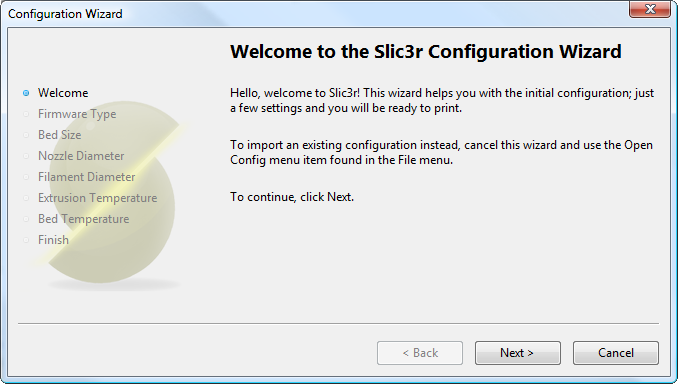
\includegraphics[keepaspectratio=true,width=\textwidth]{configuration_wizard/configuration_wizard_welcome.png}
\caption{Assistant de Configuration: \'Ecran de bienvenue}
\label{fig:configuration_wizard_welcome_screen}
\end{figure}

\newpage
\subsection{1. Type de Micrologiciel}
\label{sub:1_firmware_type}
\index{Printer Settings!Firmware!G-code flavour}
\index{Param\`etres de l'imprimante!Micrologiciel!variante du G-code}

Le G-code produit par Slic3r est adapt\'e \`a certains types de micrologiciel. La premi\`ere \'etape, demande le micrologiciel utilis\'e pour l'imprimante. Cela a d\^u \^etre sp\'ecifi\'e lorsque l'imprimante a \'et\'e construite ou configur\'ee. En cas de doute contactez le fournisseur.
\begin{figure}[H]
\centering
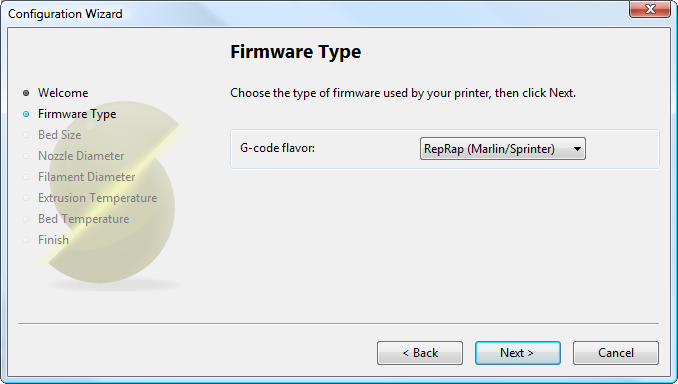
\includegraphics[keepaspectratio=true,width=\textwidth]{configuration_wizard/configuration_wizard_firmware_type.png}
\caption{Assistant de Configuration: Type de Micrologiciel}
\label{fig:configuration_wizard_firmware_type}
\end{figure}

\newpage
\subsection{2. Taille du Lit}
\label{sub:2_bed_size}
\index{Printer Settings!Size and coordinates!Bed size}
\index{Param\`etres de l'imprimante!Taille et coordonn\'ees!Taille du Lit}

Ce param\`etre d\'efinit la distance maximale que l'extrudeuse peut parcourir le long de l'axe X et Y. Si les dimensions ne sont pas disponibles, elles peuvent \^etre facilement mesur\'ee.

N'oubliez pas de mesurer \`a partir du coin inf\'erieur gauche o\`u la buse d'extrusion repose quand elle est en position de repos jusqu'a la distance maximale que la buse peut ateindre pour chaque direction. Prenez en compte que le chariot de X peut toucher le cadre avant la buse atteigne sa limite, cela d\'ependra de la marque et du mod\`ele de l'imprimante.

Pensez \'egalement \`a v\'erifier les param\`etres de but\'ee du micrologiciel, qui peuvent limiter les d\'eplacement X / Y.

\begin{figure}[H]
\centering
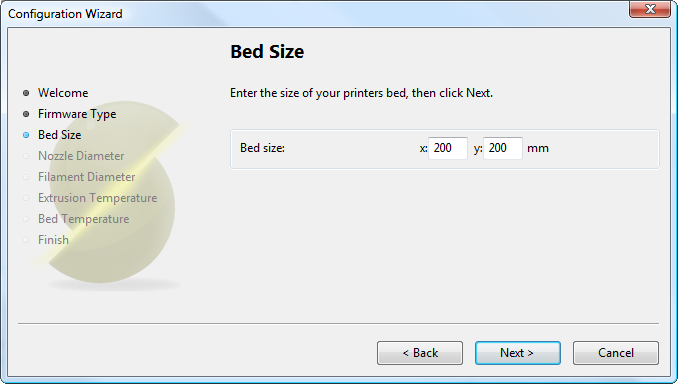
\includegraphics[keepaspectratio=true,width=\textwidth]{configuration_wizard/configuration_wizard_bed_size.png}
\caption{Assistant de Configuration: Taille du Lit}
\label{fig:configuration_wizard_bed_size}
\end{figure}

\newpage
\subsection{3. Diam\`etre de la buse}
\label{sub:3_nozzle_diameter}
\index{Printer Settings!Extruder!Nozzle diameter}
\index{Param\`etres de l'imprimante!Extrudeuse!Diam\`etre de la buse}
Traduction
Le diam\`etre de la buse est g\'en\'eralement clairement affich\'e soit dans la description de la t\^ete chauffante, ou dans la documentation associ\'ee, lorsque la t\^ete chauffante est achet\'e. Les valeurs courantes sont 0,5 mm et 0,35 mm.

Si la buse est faite maison, ou provient d'une source sans informations du diam\`etre, alors mesurez soigneusement l'ouverture aussi pr\'ecis\'ement que possible. Une fa\c{c}on de d\'eterminer la taille de la buse est d'extruder tr\`es lentement (1mm / s) un peu de filament \`a l'air libre, et de mesurer l'\'epaisseur de l'extrusion\footnote{\url{http://forums.reprap.org/read.php?1,113374,113953}}.  
Ceci a l'avantage de prendre en compte gonflement \`a la fili\`ere, et par cons\'equent pourrait \^etre une chose utile \`a faire, m\^eme si le diam\`etre est connu.

\begin{figure}[H]
\centering
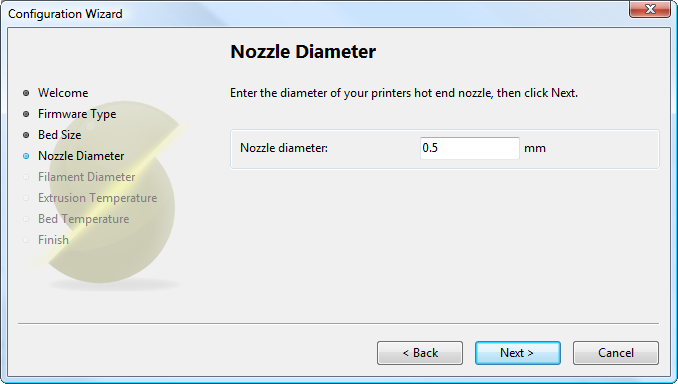
\includegraphics[keepaspectratio=true,width=\textwidth]{configuration_wizard/configuration_wizard_nozzle_diameter.png}
\caption{Assistant de Configuration: Diam\`etre de la buse}
\label{fig:configuration_wizard_nozzle_diameter}
\end{figure}

\newpage
\subsection{4. Diam\`etre du Filament}
\label{sub:4_filament_diameter}
\index{Filament Settings!Filament!Diameter}
\index{Param\`etres du Filament!Filament!Diam\`etre}
Pour que Slic3r produise des r\'esultats pr\'ecis, il doit conna\^itre aussi pr\'ecis\'ement que possible la quantit\'e de mati\`ere qui est pouss\'e \`a travers l'extrudeuse. Il est donc essentiel de lui donner la valeur la plus pr\'ecise possible pour le diam\`etre du filament.

Bien que le filament utilis\'e dans les imprimantes FDM soit vendu pour un diam\`etre de 3 mm ou 1,75 mm ce n'est qu'une indication . Le diam\`etre peut varier entre les fabricants et m\^eme entre les lots. Par cons\'equent, il est fortement recommand\'e de prendre des mesures multiples de long du filament et utiliser la moyenne. Par exemple, les mesures de 2.89, 2.88, 2.90 et 2.91 donneraient une moyenne de 2,895, \`a utiliser ici.

\begin{figure}[H]
\centering
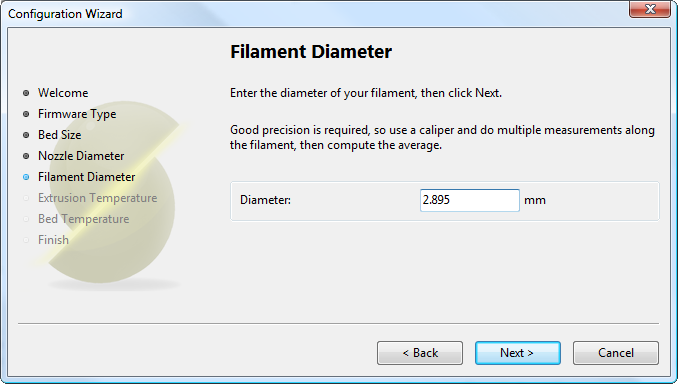
\includegraphics[keepaspectratio=true,width=\textwidth]{configuration_wizard/configuration_wizard_filament_diameter.png}
\caption{Assistant de Configuration: Diam\`etre du Filament}
\label{fig:configuration_wizard_filament_diameter}
\end{figure}

\newpage
\subsection{5. Temp\'erature d'Extrusion}
\label{sub:5_extrusion_temperature}
\index{Filament Settings!Temperature!Extruder}
\index{Param\`etres du Filament!Temperature!Extrudeuse}
La temp\'erature d'extrusion d\'epend de la mati\`ere, celles-ci peuvent fonctionner sur une large plage de temp\'erature. Le fournisseur doit fournir des informations sur les temp\'eratures appropri\'es. Une r\`egle tr\`es g\'en\'erale est que la temp\'erature pour le PLA est comprise entre 160 ° C et 230 ° C, et que la temp\'erature pour l'ABS se situe entre 215 ° C et 250 ° C. Les mat\'eriaux plus exotiques auront une gamme diff\'erente.

C'est un param\`etre que vous aurez envie de peaufiner quand vous commencerez \`a produire des impressions. La temp\'erature optimale peut varier, m\^eme entre les couleurs de la m\^eme mati\`ere. Un autre facteur qui peut affecter la temp\'erature choisie, est la vitesse d'extrusion, g\'en\'eralement plus la vitesse est \'elev\'e, plus la temp\'erature est \'elev\'ee.

Remarque: On peut choisir de r\'eguler la temp\'erature de l'extrudeuse manuellement \`a partir du contr\^oleur d'imprimante. Dans ce cas, la temp\'erature peut \^etre r\'egl\'ee \`a z\'ero.

\begin{figure}[H]
\centering
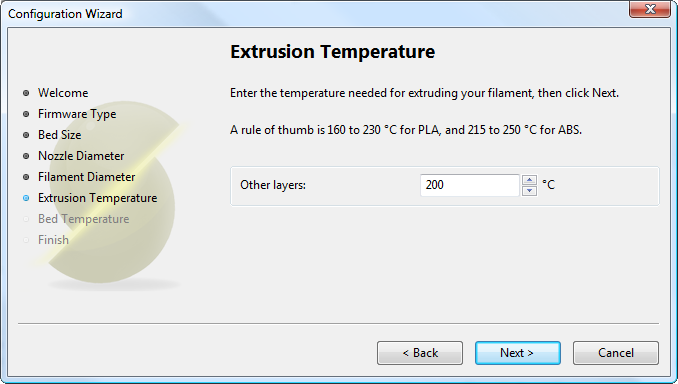
\includegraphics[keepaspectratio=true,width=\textwidth]{configuration_wizard/configuration_wizard_extrusion_temperature.png}
\caption{Assistant de Configuration: Temp\'erature d'Extrusion}
\label{fig:configuration_wizard_extrusion_temperature}
\end{figure}

\newpage
\subsection{6. Temperature du Lit}
\label{sub:6_bed_temperature}
\index{Filament Settings!Temperature!Bed}
\index{Param\`etres du Filament!Temperature!Lit}
Si l'imprimante dispose d'un lit chauff\'e ce param\`etre peut \^etre pr\'ecis\'e. Comme la temp\'erature de l'extrudeuse, la valeur d\'epend de la mati\`ere utilis\'ee. Une r\`egle de base est que PLA n\'ecessite ~ 60 ° C et ABS n\'ecessite ~ 110 ° C.

Remarque: On peut choisir de contr\^oler la temp\'erature du lit manuellement \`a partir du contr\^oleur d'imprimante. Dans ce cas, la temp\'erature peut \^etre r\'egl\'ee \`a z\'ero.

\begin{figure}[H]
\centering
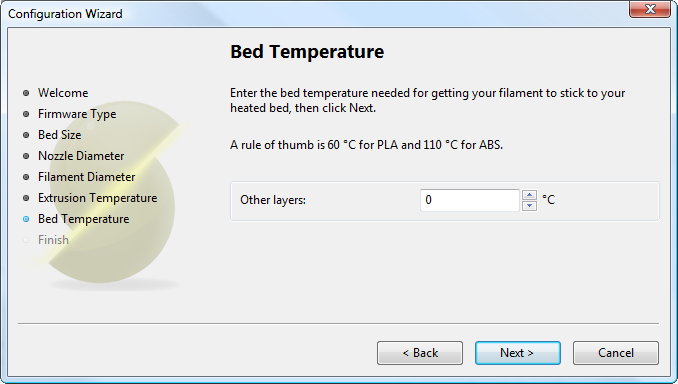
\includegraphics[keepaspectratio=true,width=\textwidth]{configuration_wizard/configuration_wizard_bed_temperature.png}
\caption{Assistant de Configuration: Temperature du Lit}
\label{fig:configuration_wizard_bed_temperature}
\end{figure}

\newpage

A ce stade, l'assistant est termin\'e et la configuration de base est d\'efinie.

\begin{figure}[H]
\centering
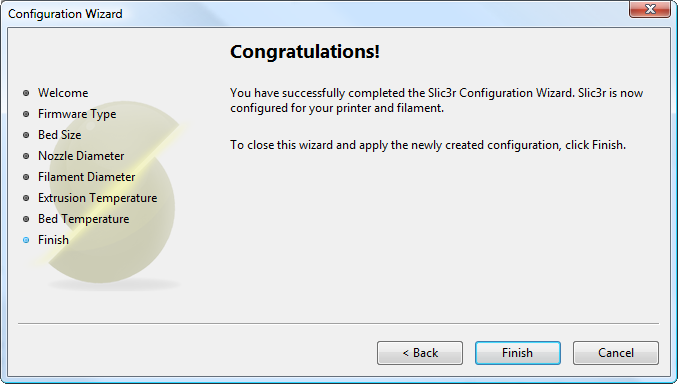
\includegraphics[keepaspectratio=true,width=\textwidth]{configuration_wizard/configuration_wizard_end.png}
\caption{Assistant de Configuration: Fin}
\label{fig:configuration_wizard_end}
\end{figure}



\newpage

%!TEX root = Slic3r-Manual.tex

\section{"La" Première Couche}
\label{sec:the_important_first_layer}
\index{First Layer}
\index{Première Couche}

Avant de se lancer tête baissée dans dans la production de la première impression, il est intéressant de s'arreter pour parler de l'importance d'obtenir une première couche parfaite. Comme beaucoup l'ont constaté par tâtonnements, si la première couche n'est pas la meilleure, cela peut alors conduire à un échec complet, des parties se détachant, et des déformations. Il existe plusieurs techniques et recommandations, dont on peut tenir compte afin de minimiser le risque que cela se produise.

\paragraph{Le lit à niveau} % (fold)
\label{par:level_bed}
Avoir un lit de niveau est essentiel. Si la distance entre l'extrémité de la buse et le lit diffèrre de même quelque microns, il se peut que la matière ne soit pas étendue sur le lit (parce que la buse est trop proche et racle le lit), ou que de la matière se trouvant trop eloignée du lit, n'adhére pas correctement.
% paragraph level_bed (end)

\paragraph{Température plus élevée.} % (fold)
\label{par:higher_temperature}
La tête chauffante et le lit, s'il est chauffé, peuvent être surchauffés pour la première couche, ceci diminue la viscosité de la matière en cours d'impression.  En règle générale, un supplément de 5 ° est recommandé.
% paragraph higher_temperature (end)

\paragraph{Des vitesses inférieures.} % (fold)
\label{par:lower_speeds}
Ralentir l'extrudeuse pour la première couche réduit les efforts appliqués à la matière fondue à la sortie, ce qui réduit les chances d'être trop étirées et de ne pas adhérer correctement. 30\% ou 50\% de la vitesse normale est recommandée.
% paragraph lower_speeds (end)

\paragraph{Taux d'extrusion correctement calibré.} % (fold)
\label{par:correct_extrusion_settings}
Si trop de matière est extrudé alors la buse peut glisser par dessus lors du deuxième passage, en la soulevant par rapport au lit (en particulier si le matériau a refroidi). Trop peu de matière peut faire que la première couche se détache plus tard lors de l'impression, conduisant soit à arrachements ou des déformations. Pour ces raisons, il est important d'avoir un taux d'extrusion bien calibré tel que recommandé au §\ref{calibration}).
% paragraph correct_extrusion_settings (end)

\paragraph{La hauteur de la première couche.} % (fold)
\label{par:first_layer_height}
Une couche épaisse fournira plus de débit, et par conséquent plus de chaleur, ce qui permet à l'extrusion de mieux adhérer au lit. Elle donne aussi l'avantage d'apporter plus de tolérance pour la planéité du lit. Il est recommandé d'augmenter la hauteur de la première couche pour correspondre au diamètre de la buse, par exemple, une première hauteur de la couche de 0,35 mm pour une buse 0.35mm.
Remarque: La hauteur de la première couche est automatiquement réglée de cette façon en mode simple.
% paragraph first_layer_height (end)

\paragraph{Plus grossse largeur d'extrusion.} % (fold)
\label{par:wider_extrusion_width}
Plus il y a de matière à toucher le lit, plus l'objet adhère au lit, ceci peut être obtenu en augmentant la largeur de l'extrusion de la première couche, soit par un pourcentage ou une quantité fixée. Les espaces entre les extrusions sont ajustés en conséquence.

Une valeur d'environ 200 \% est généralement recommandée, mais il faut noter que la valeur est calculée à partir de la hauteur de la couche et donc la valeur ne doit être réglée que si la hauteur de la couche est la plus élevée possible. Par exemple, si la hauteur de la couche est de 0,1 mm, et que la largeur de l'extrusion est réglée à 200 \%, alors la largeur réelle extrudé sera seulement de 0,2 mm, ce qui est plus petite que la buse. Cela risque de provoquer un mauvais écoulement et conduire à une impression ratée. Il est donc fortement recommandé de combiner la hauteur de la première couche, recommandée ci-dessus avec celle-ci. Régler la hauteur de la première couche à 0,35 mm et la première largeur d'extrusion à 200 \% se traduirait par une belle grosse extrusion 0,65 mm de large.
% paragraph wider_extrusion_width (end)

\paragraph{Matériau du lit.} % (fold)
\label{par:bed_material}
Plusieurs solutions existent pour le matériel à utiliser pour le lit, et la préparation de la surface peut considèrablement améliorer l'adhérence de la première couche.

Le PLA est plus tolérant et fonctionne bien sur le PET, Kapton, ou ruban adhèsif de peintre bleu.


L'ABS a généralement besoin de plus d'attentions et, s'il s'imprime bien sur PET et Kapton, on rapporte que les gens ont de bon résultats en appliquant de la laque sur le lit avant de l'imprimer. D'autres ont signalé qu'une solution d'ABS (fabriqué à partir de la dissolution de morceaux d'ABS dans de l'acétone) finement appliquée peut également augmenter l'adhèrence.
% paragraph bed_material (end)

\paragraph{Aucun refroidissement.} % (fold)
\label{par:no_cooling}
Directement lié à ce qui précède, il n'est pas logique d'augmenter la température de la première couche et avoir un ventilateur ou un autre mécanisme de refroidissement en fonctionement. Garder le ventilateur éteint pendant les quelques premières couches est généralement recommandé.
% paragraph no_cooling (end)


\newpage

%!TEX root = Slic3r-Manual.tex
\section{Travailler avec les mod\`eles 3D}
\label{sub:working_with_models}
\index{models}
\index{mod\`eles 3D}

Il reste encore une \'etape avant la prmi\`ere impression: obtenir un mod\`ele 3D et le "trancher".

\subsection{Formats de Mod\`eles 3D} % (fold)
\label{sub:model_formats}
\index{STL}
\index{AMF}
\index{OBJ}

Slic3r accepte les types de fichiers suivants.

\begin{itemize}
	\item Les fichiers ST\'er\'eolithographique (STL) peuvent provenir d'une grande vari\'et\'e de sources et sont maintenant un standard de facto dans l'impression 3D. Les fichiers d\'ecrivent simplement la g\'eom\'etrie de la surface d'un objet 3D sans aucune information suppl\'ementaire (comme la couleur ou la mati\`ere), et c'est cette simplicit\'e qui a probablement fait le format omnipr\'esent.
	\item Le type de fichier Wavefront OBJ est un format ouvert utilis\'e \`a l'origine dans une application d'animation de Wavefront Technologies, mais a depuis \'et\'e adopt\'ee par la communaut\'e de la mod\'elisation 3D. Il est similaire au format STL.
	\item Le format de fichier AMF (Additive Manufacturing File Format) a \'et\'e d\'evelopp\'e en r\'eponse au caract\`ere limit\'e du format STL. En plus de d\'ecrire la g\'eom\'etrie du mod\`ele 3D, il peut \'egalement d\'ecrire les couleurs et les mat\'eriaux, ainsi que des attributs plus complexes, tels que les m\'elanges d\'egrad\'e et de multiples arrangements d'objets (constellations). Alors que le format est consid\'er\'e comme un standard, il reste \`a \^etre largement adopt\'ee dans le milieu de la machine 3D.
\end{itemize}
% subsection model_formats (end)

\subsection{Trouver des Mod\`eles 3D} % (fold)
\label{sub:finding_models}
\index{models!finding}
\index{mod\`eles!trouver}

Les fichiers de mod\`ele 3D peuvent provenir d'un d\'ep\^ot en ligne, tels que Thingiverse\footnote{\url{http://www.thingiverse.com}} ou GrabCAD\footnote{\url{http://grabcad.com}}, ou \^etre cr\'e\'ee \`a partir d'un programme de CAO, comme FreeCAD\footnote{\url{http://sourceforge.net/projects/free-cad}}, Sketchup\footnote{\url{http://www.sketchup.com}}, ou OpenSCAD\footnote{\url{http://www.openscad.org}}, ou un outil de CAO en ligne tels que Shapesmith\footnote{\url{http://shapesmith.net}}.

Vous souhaitez peut-\^etre afficher les fichiers avant de trancher et il ya beaucoup d'applications disponibles, dont l'un est Meshlab\footnote{\url{http://www.meshlab.org}} - un outil complet pour la visualisation et la manipulation des fichiers 3D.

\begin{figure}[H]
\centering
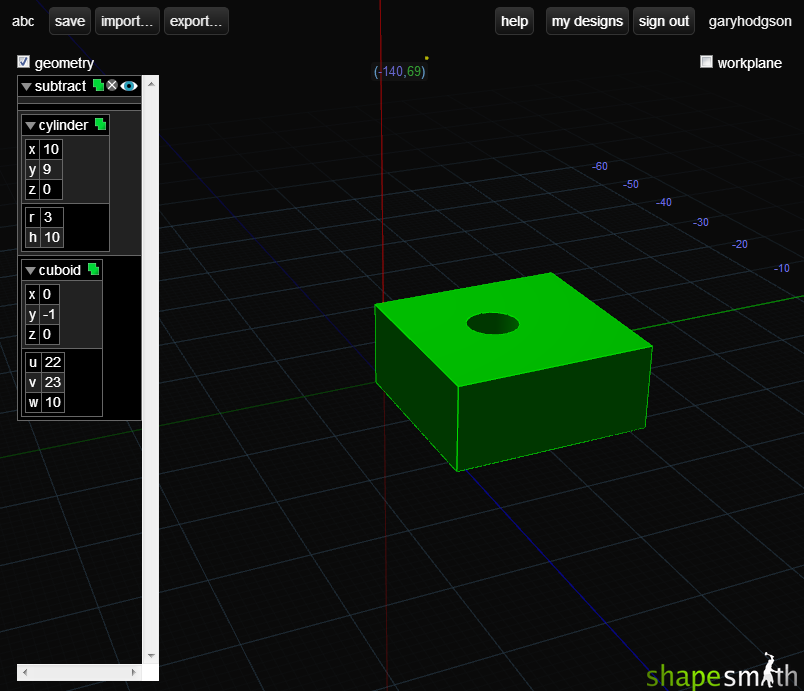
\includegraphics[keepaspectratio=true,width=0.75\textwidth]{working_with_models/shapesmith.png}
\caption{Outil de CAO en ligne Shapesmith.}
\label{fig:shapesmith}
\end{figure}

% subsection working_with_models (end)


\subsection{Utiliser la Surface de Travail} % (fold)
\label{sub:working_with_plater}
\index{Plater}
\index{Surface de Travail}
Slic3r dispose d'un outil, appel\'e Plater, qui permet \`a un ou plusieurs mod\`eles \`a \^etre charg\'es et dispos\'es avant d'\^etre "tranch\'es".

\begin{figure}[H]
\centering
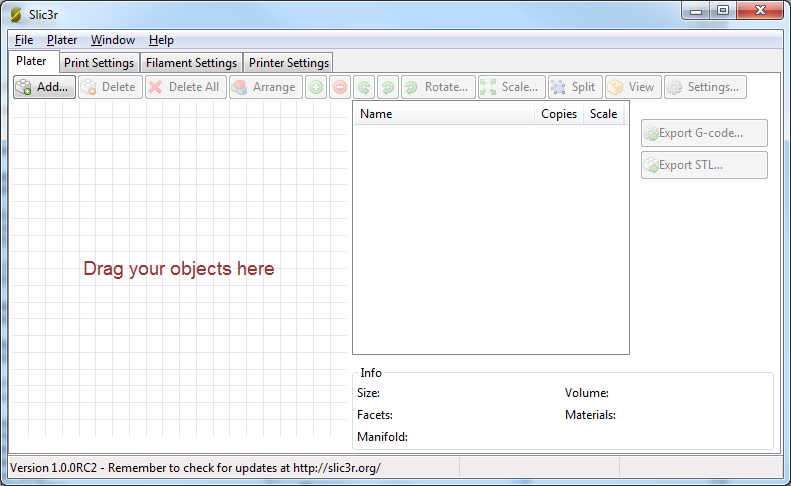
\includegraphics[keepaspectratio=true,width=1\textwidth]{working_with_models/plater.png}
\caption{Surface de Travail}
\label{fig:plater}
\end{figure}


Une fois que vous avez acquis un mod\`ele, faites-le glisser sur l'onglet "Plater" (ou utilisez le bouton Add(Ajouter) dans le coin supp\'erieur gauche) pour le charger dans Slic3r. Dans la figure ci-dessous, la traditionnelle RepRap Minimug\footnote{\url{http://www.thingiverse.com/thing:18357}} is loaded, and is viewed from above. The ring around the model is a skirt - a single perimeter, several millimeters away from the model, which is extruded first.  This is useful in making sure the plastic is flowing smoothly from the nozzle when the model is starting to be printed.

\begin{figure}[H]
\centering
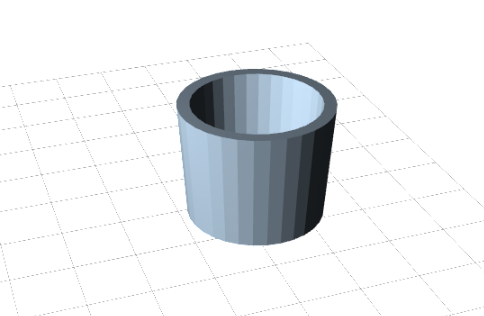
\includegraphics[keepaspectratio=true,width=0.75\textwidth]{working_with_models/minimug_model.png}
\caption{Le Mod\`ele Minimug.}
\label{fig:minimug_model}
\end{figure}

\begin{figure}[H]
\centering
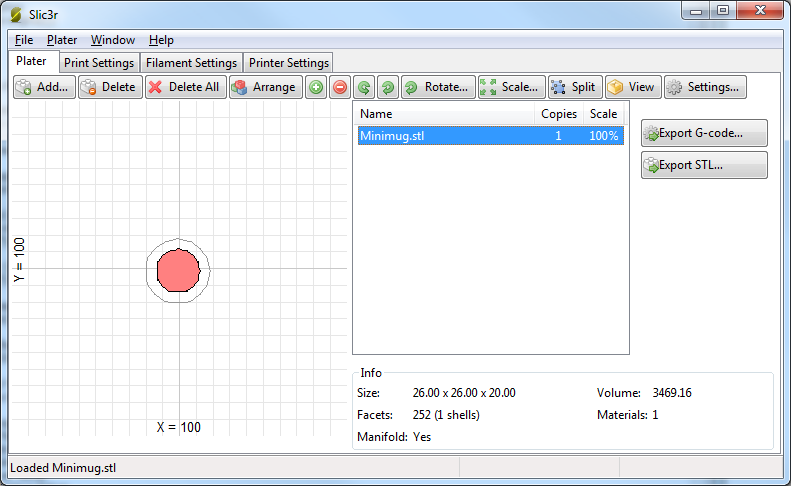
\includegraphics[keepaspectratio=true,width=1\textwidth]{working_with_models/plater_model_loaded.png}
\caption{Fichier STL charg\'e.}
\label{fig:plater_model_loaded}
\end{figure}

Le mod\`ele peut \^etre repositionn\'ee en le d\'eplaçant sur la repr\`esentation du lit \`a gauche de l'\'ecran. Notez que les dimensions du lit doivent correspondre \`a votre imprimante, tel qu'elles sont donn\'ees lors de la configuration initiale ci-dessus.

Sur le c\^ot\'e droit il y a la liste des fichiers actuellement charg\'es. Les boutons situ\'es en haut de la liste de fichier vous permettent d'organiser les mod\`eles.
\begin{itemize}
	\item \textbf{More/Less (plus/moins)}  - R\'egle le nombre de copies qui doit \^etre imprim\'e.
	\item \textbf{45°/Rotate (45°/rotation)}  - Fait pivoter le mod\`ele s\'electionn\'e autour de l'axe Z, soit de 45 ° dans le sens horaire ou anti-horaire, ou par une valeur donn\'ee.
	\item \textbf{Scale (\'echelle)}  - Augmenter ou diminuer la taille du mod\`ele imprim\'e.
	\item \textbf{Split (dissocier)}  - Divise un mod\`ele qui se compose de plus d'une partie en ses parties constituantes, ce qui permet \`a chacune d'\^etre agenc\'ee individuellement.
\end{itemize}


Les boutons en haut \`a gauche, vous permettent d'ajouter, de supprimer, d'auto-organiser, ou d'exporter les mod\`eles.
\begin{itemize}
	\item \textbf{Add (Ajouter)}  - Ouvre une bo\^ite de dialogue pour ajouter un mod\`ele \`a la surface de travail, c'est une alternative gliss\'e/d\'epos\'e du fichier sur la surface de travail.
	\item \textbf{Delete/Delete All (Supprimer/Tout supprimer)}  - Retirer un ou tous les mod\`eles de la surface de travail.
	\item \textbf{Autoarrange}  - Essaye d'organiser les mod\`eles pour obtenir l'agencement optimal.
	\item \textbf{Export G-code}  - D\'emarre le "tranchage" du mod\`ele, et produit un fichier G-code.
	\item \textbf{Export STL}  - Sauvegarde un ensemble de mod\`ele de la surface de travail dans un fichier STL unique.
\end{itemize}


% subsection working_with_plater (end)

\subsection{R\'eparer les fichiers STL} % (fold)
\label{sub:cleaning_stls}
\index{STL!cleaning}
\index{STL!r\'eparer}
Si le maillage 3D d\'ecrit dans le mod\`ele contient des trous, ou les bords ne sont pas align\'es (connu comme \'etant non-manifold), puis Slic3r peut avoir des probl\`emes pour le traiter. Slic3r va tenter de r\'esoudre les probl\`emesqu'il peut, mais certains probl\`emes sont hors de sa port\'ee. Si l'application se plaint que le mod\`ele ne peut pas \^etre "tranch\'e" correctement alors il ya plusieurs options possibles: voir le chapitre sur la R\'eparation des mod\`eles.

% subsection cleaning_stls (end)

\newpage

%!TEX root = Slic3r-Manual.tex

\section{Printing} % (fold)
\label{sec:printing}
\index{Printing}

At this stage Slic3r has been configured and a model has been acquired, sliced and made ready for print.  Now would be the time to fire up the printer and try it out.

A variety of host software is available to send the G-code to the printer.  Amongst the open-source solutions are: Printrun\footnote{https://github.com/kliment/Printrun}, Repetier\footnote{http://www.repetier.com/} and Repsnapper\footnote{https://github.com/timschmidt/repsnapper}.

The following sections will cover the options available in expert mode, and look at advanced printing techniques, including special cases and troubleshooting.

% section first_print (end)
}
\fi
%%% END FIRST PRINT %%%

%%% SIMPLE MODE %%%
\ifgetting
\chapter{\emph{Mode Simple}}
\thispagestyle{empty}
\markboth{Mode Simple}{Manuel Utilisateur de Slic3r}
{%!TEX root = Slic3r-Manual.tex
\section{Simple Mode} % (fold)
\label{sec:simple_mode}
\index{simple mode}

Slic3r has two modes of operation, Simple and Expert. These may be chosen from the \texttt{Preferences} window (found under the \texttt{File} menu).

\begin{figure}[ht]
\centering
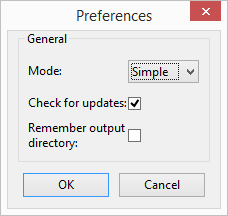
\includegraphics[width=0.3\textwidth]{simple_mode/preferences_general.png}
\caption{Preferences.}
\label{fig:preferences_general}
\end{figure}

Simple mode offers a reduced set of options, enough for the beginner to get started with.  Expert mode give more control over how Slic3r produces the G-code and will be looked at later.

\subsection{Print Settings}
\index{Print Settings}

The \texttt{Print Settings} tab provides the opportunity to change settings related to the actual print.  Whereas the other tabs are changed rarely, the settings on this tab will be modified regularly, possibly for each model printed.

\begin{figure}[ht]
\centering
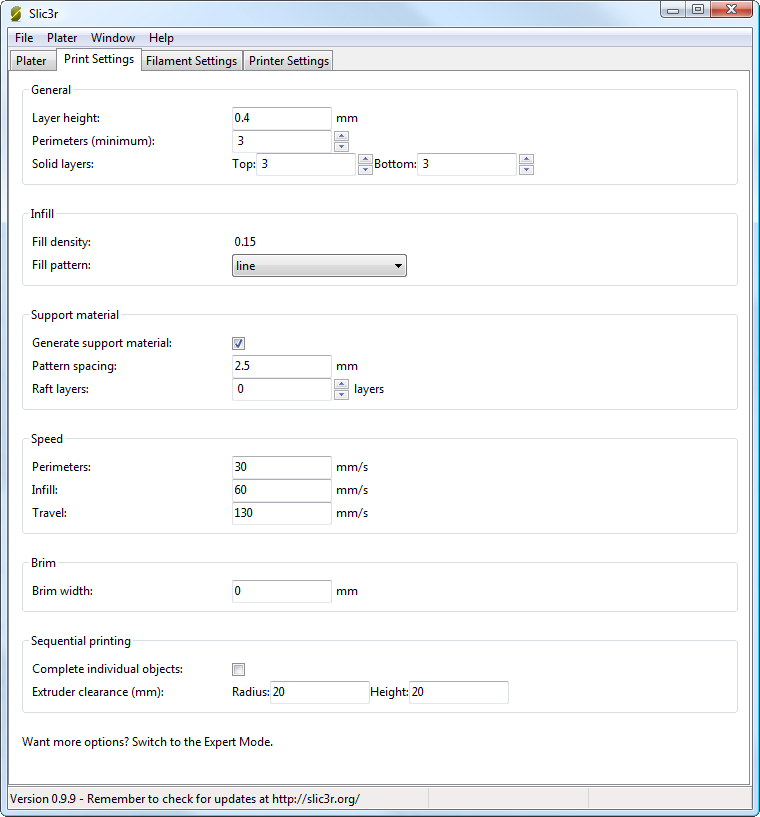
\includegraphics[width=\textwidth]{simple_mode/simple_mode_print_settings.png}
\caption{Simple Mode: Print Settings.}
\label{fig:simple_mode_print_settings}
\end{figure}

\paragraph{General.} % (fold)
\label{par:simple_general}
\index{Print Settings!Layer height}

\texttt{Layer height} is the thickness of each layer, and it is the step along the vertical axis taken before extruding a new layer atop the previous one.  There are several factors that influence how high each layer should be:
\begin{itemize}
	\item \textbf{Desired resolution}  - Lower layer height should result in prints with less noticeable ribs or bands, as each layer is smaller.  Aesthetics plays a role here, but also the type of model, for example, a mechanical part may not need such a high resolution finish, whereas a presentation piece may do so.
	\item \textbf{Print speed}  - Shorter layers will result in smoother prints but each print will take longer, simply because the extruder must trace the pattern more times.  A later goal will be to strike a balance between layer height, the speed of the printer, and the quality of the resulting print.
\end{itemize}
\index{Print Settings!Perimeters}
\texttt{Perimeters} defines the minimum number of vertical shells (i.e. walls) a print will have.  Unless the model requires single width walls it is generally recommended to have a minimum of two perimeters as this gives some insurance that if a section of the perimeter is not printed correctly then the second perimeter will help cover it.

\index{Print Settings!Solid layers}
The upper and lowermost layers that sandwich the model are filled with a \texttt{Solid layers} pattern.  For the bottom layers the important factor to consider is how the surface will look should there be a mistake whilst laying down the first layer, and for this reason it is recommended to have at least two bottom layers.

A similar consideration is required for the top layers.  Because the intermediate layers are likely to be filled with a pattern set less than 100\% then the covering layers will have to bridge this pattern and this can require more than one pass to cover completely.

\begin{figure}[H]
\centering
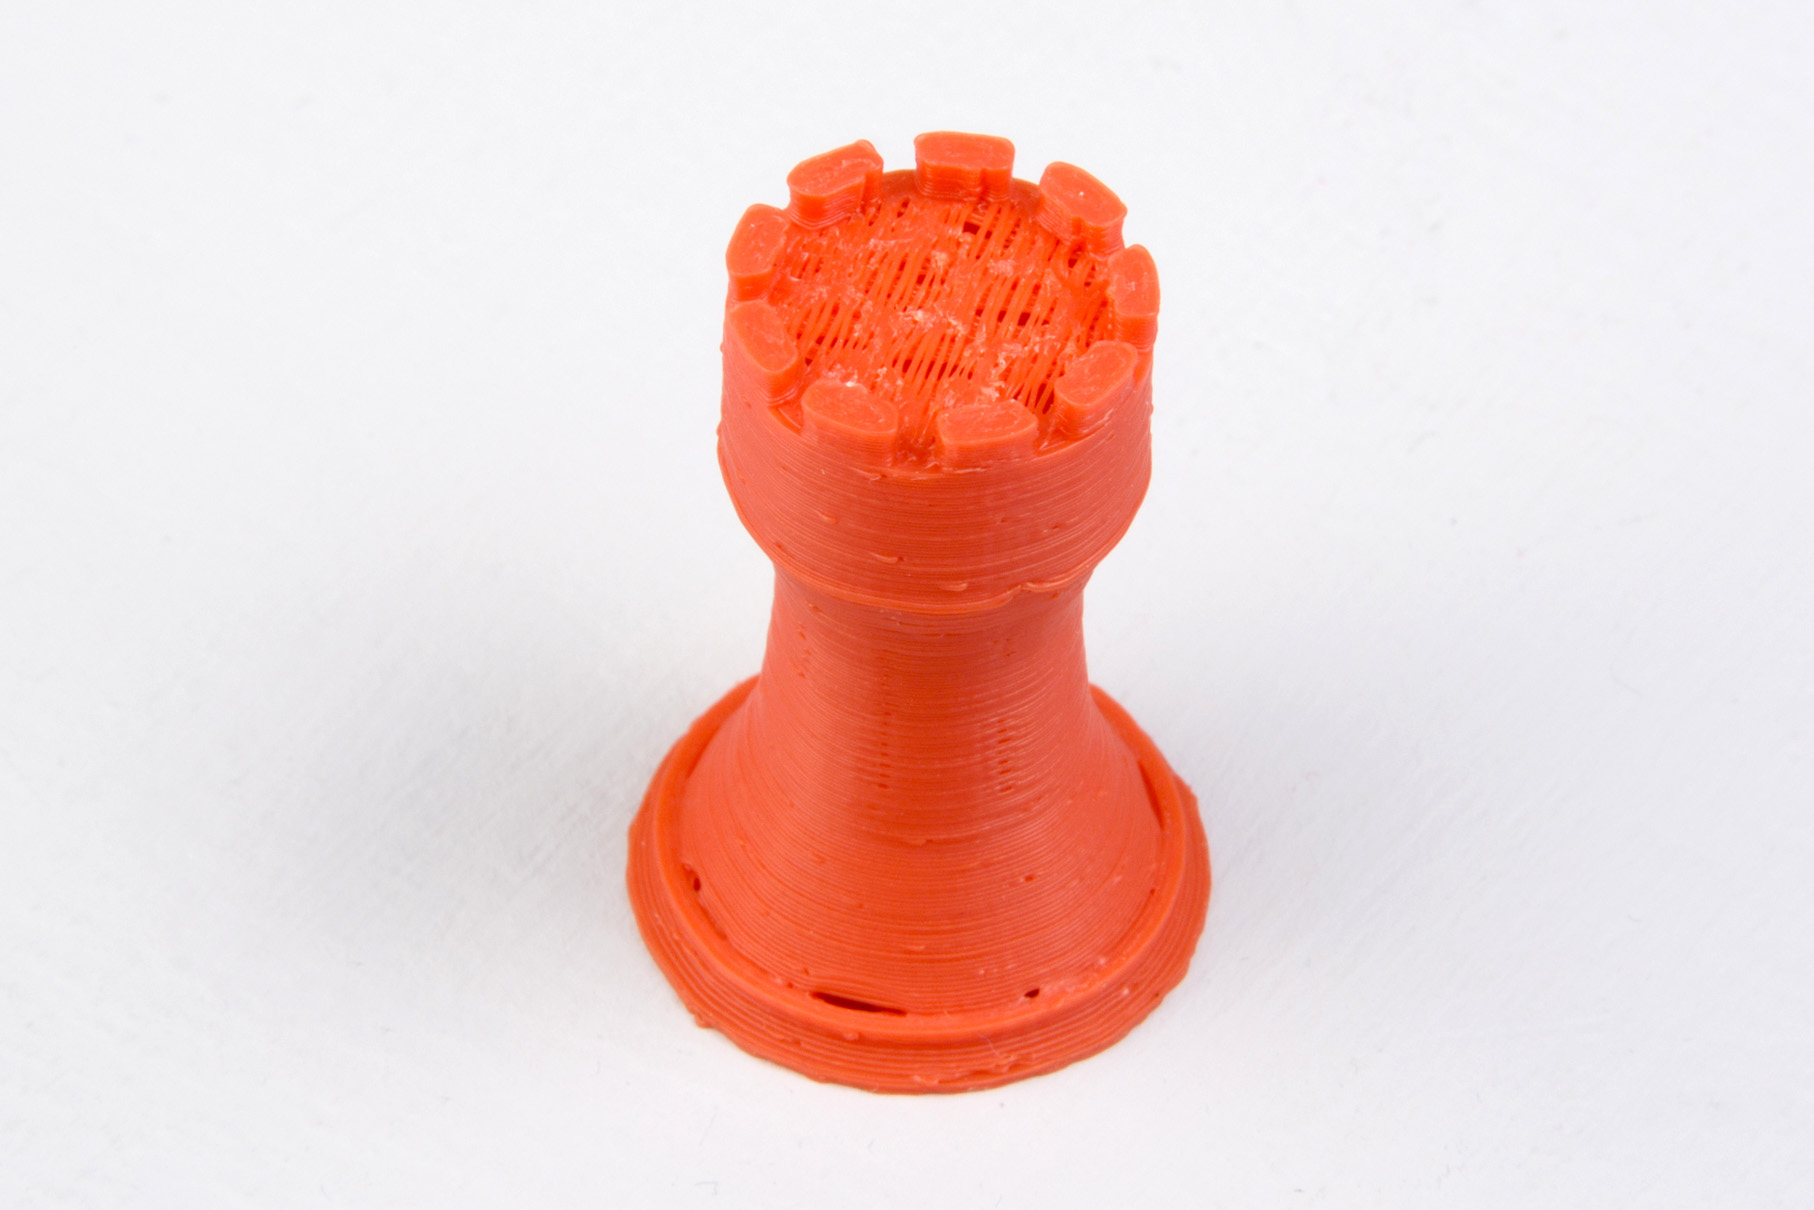
\includegraphics[keepaspectratio=true,width=0.75\textwidth]{simple_mode/bad_top_infill.jpg}
\caption{An example of insufficient top layers.}
\label{fig:bad_top_infill}
\end{figure}

Another tip to consider: Setting the top solid layer to zero, and setting the infill also to zero, will result in a hollow receptacle, ideal for turning models into vases\footnote{http://slic3r.org/blog/tip-printing-vases} for example.  Here manipulating the settings within Slic3r can be used to generate different kinds of prints, and not only be used to control surface accuracy.

\begin{figure}[H]
\centering
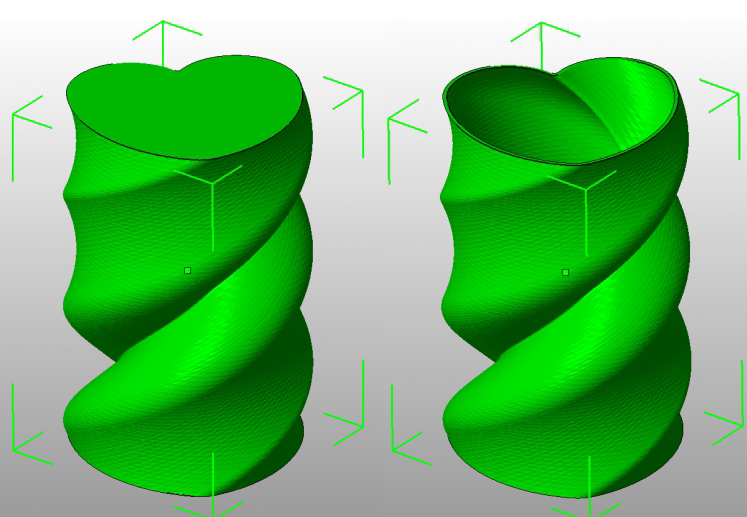
\includegraphics[keepaspectratio=true,width=0.75\textwidth]{simple_mode/solid_layers_vases.png}
\caption{Creating a vase from a solid model.}
\label{fig:solid_layers_vases}
\end{figure}

% paragraph general (end)

\paragraph{Infill.} % (fold)
\label{par:simple_infill}
\index{Print Settings!Infill}
\index{Print Settings!Infill!Fill density}
\texttt{Fill density} is defined on a scale of between 0 and 1, where 1 is 100\% and 0.4 would be 40\%.  For the majority of cases it makes no sense to 100\% fill the model with plastic, this would be a waste of material and take a long time.  Instead, most models can be filled with less material which is then sandwiched between layers filled at 100\% (see \texttt{Solid layers} above).

A density value of 0.4 is enough to give almost all models good mechanical strength.  A value of 0.2 is usually the minimum required to support flat ceilings.

\index{Print Settings!Infill!Fill pattern}
Slic3r offers several fill patterns which will be discussed in more depth in section \ref{sec:infill_patterns_and_density} - Infill Choices.  Choosing a \texttt{Fill pattern} will depend on the kind of model, the desired structural  strength, print speed, and personal taste.  The more exotic fill methods are usually too slow and unnecessarily complex for most use cases, and so most of the time the infill pattern is either \texttt{rectilinear}, \texttt{line}, or \texttt{honeycomb}.  Honeycomb gives the most strength but is slower than both rectilinear or line.

% paragraph infill (end)

\paragraph{Support material.} % (fold)
\label{par:simple_support_material}
\index{Print Settings!Support material}
\index{Print Settings!Support material!Generate support material}
\index{Print Settings!Support material!Pattern spacing}
Printing a model from the bottom up, as with FDM, means that any significant overhangs will be printed in the air, and most likely droop or not print correctly.  Choosing support material (\texttt{Generate support material}) will add additional structures around the model which will build up to then support the overhanging part.  The \texttt{Pattern spacing} option determines how dense the support material is printed.

\begin{figure}[H]
\centering
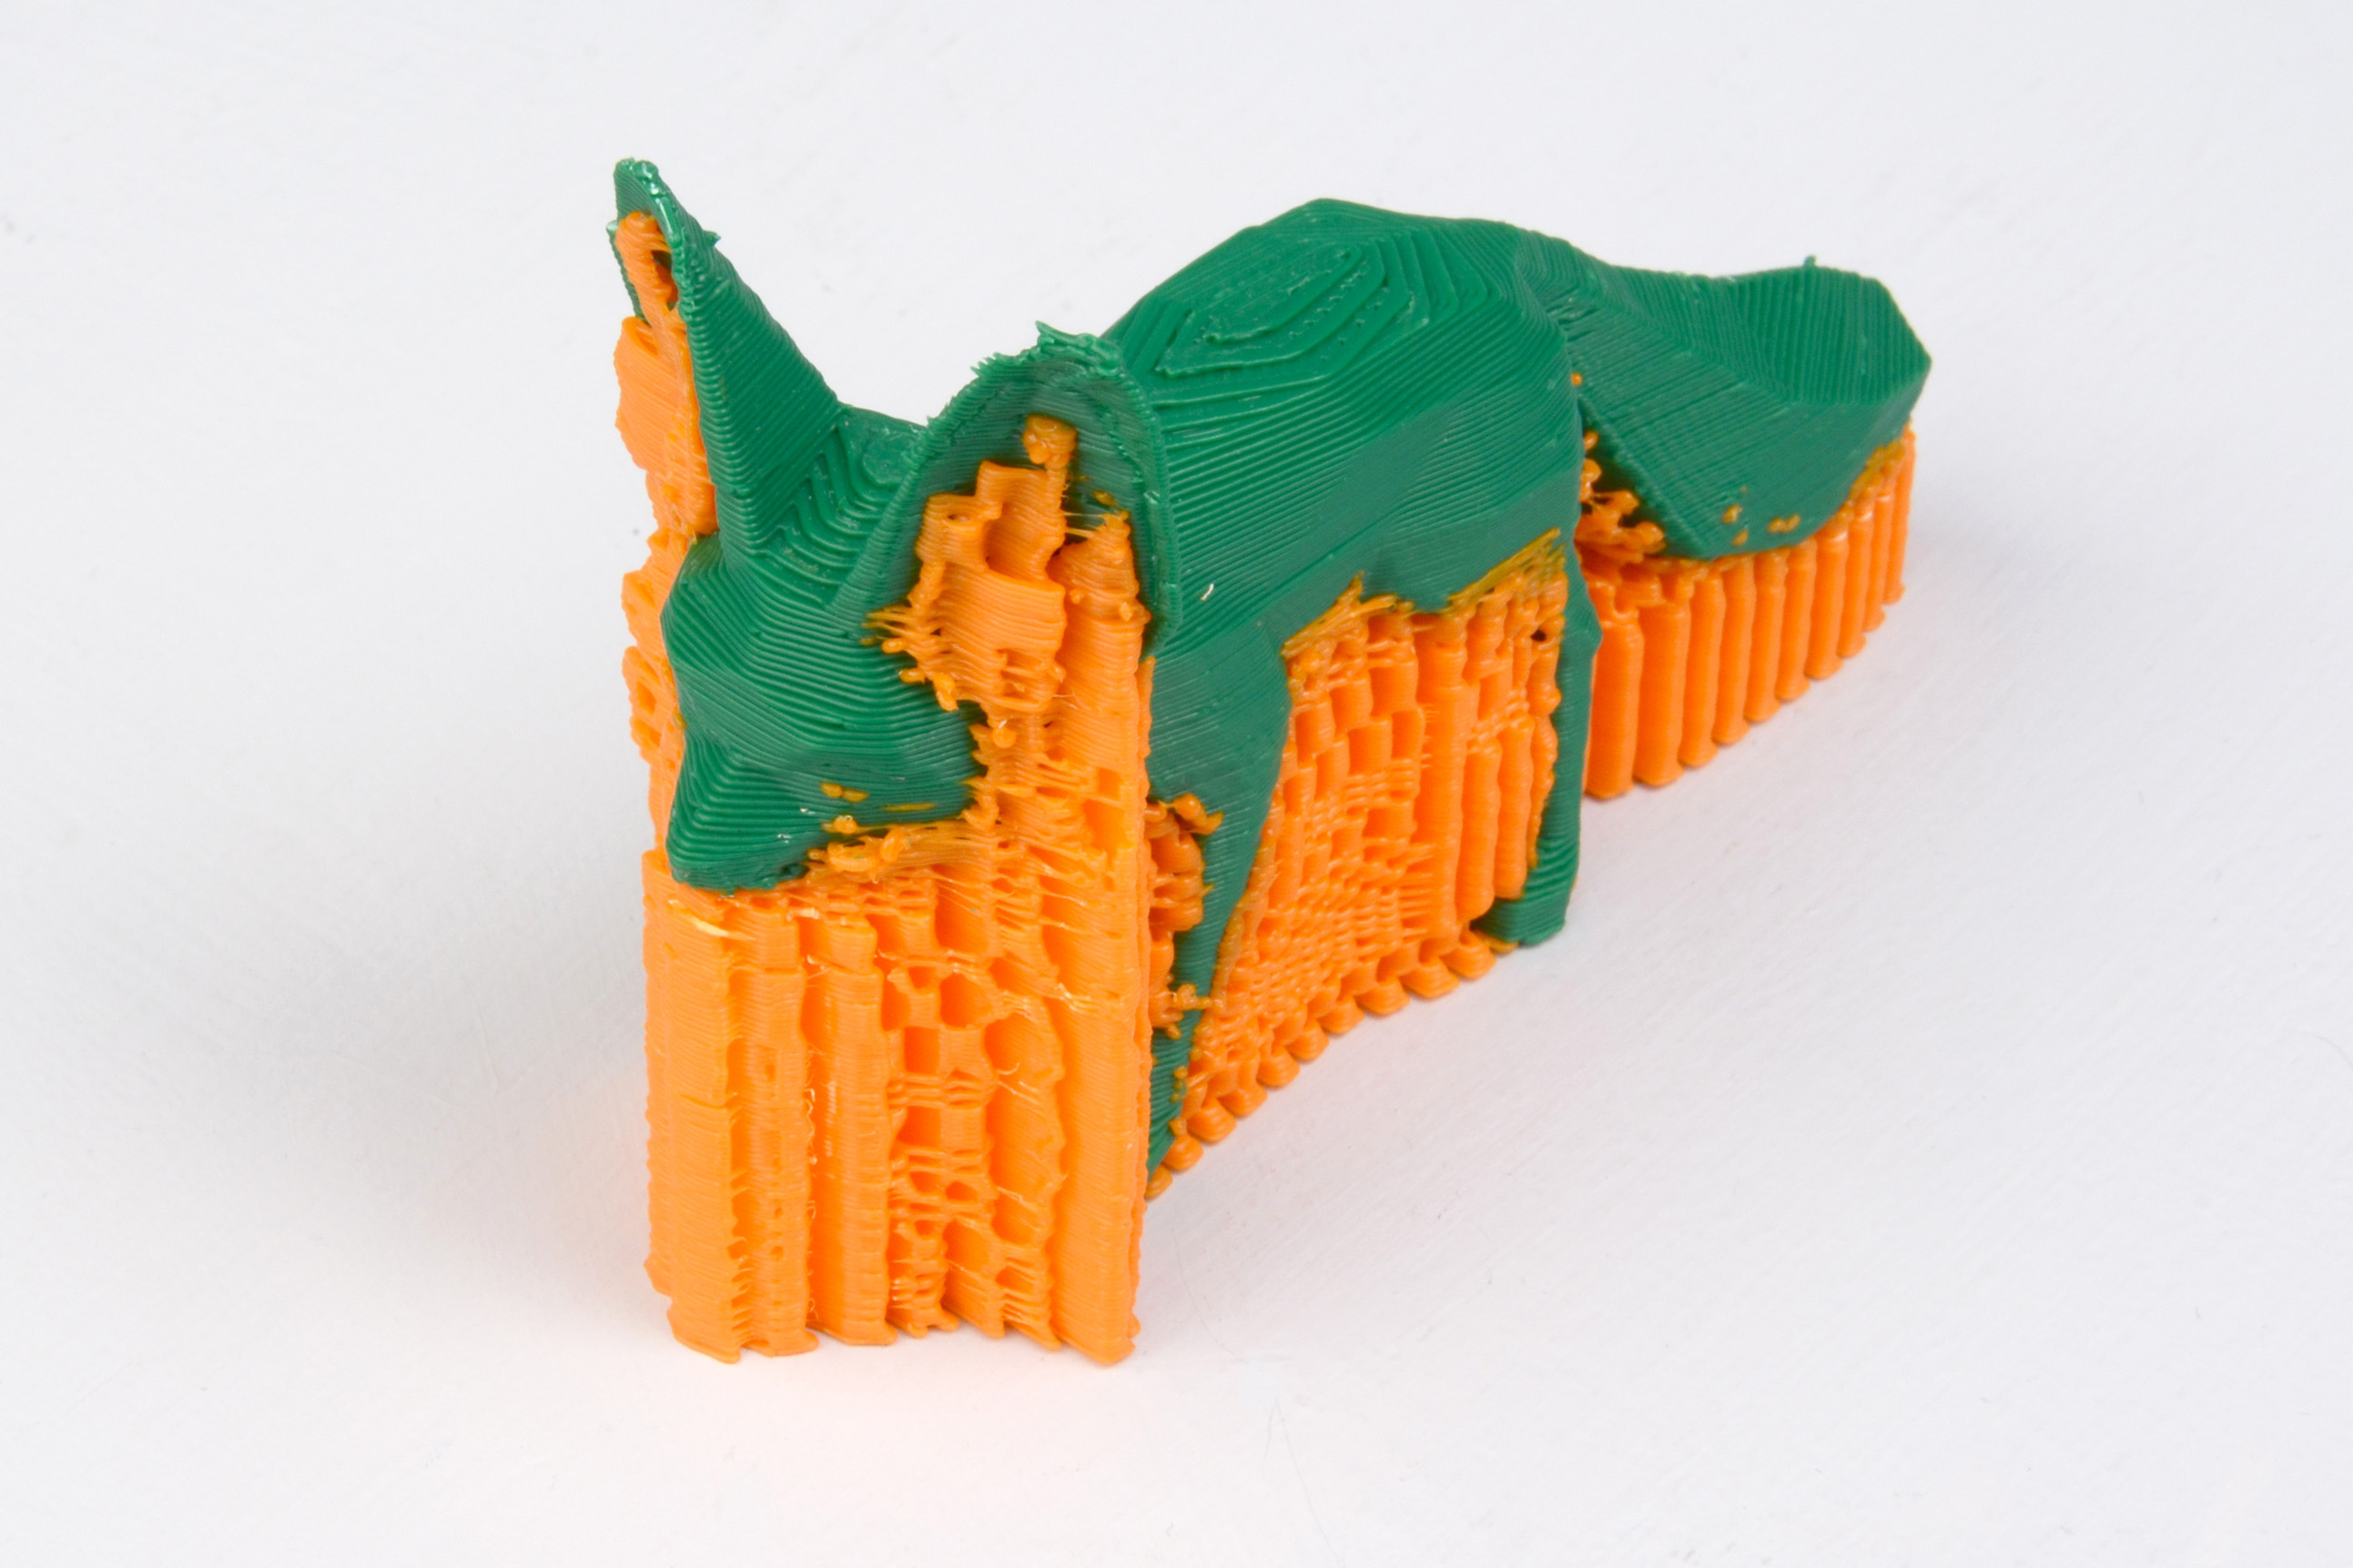
\includegraphics[keepaspectratio=true,width=0.75\textwidth]{simple_mode/support_example.jpg}
\caption{An example of an object printed with support material.}
\label{fig:support_example}
\end{figure}

Tip: It is sometimes worth considering altering the orientation of the model in order to possibly reduce overhangs.

\index{Print Settings!Support material!Raft layers}
\texttt{Raft layers} will add additional layers underneath the model and stems from the early days of 3D printing.  It can help with prints without a heated bed, or where the bed is not very flat, but it is usually not required and is not recommended.  The raft also requires post-processing to remove it.
% paragraph support_material (end)

\paragraph{Speed.} % (fold)
\label{par:simple_speed}
\index{Print Settings!Speed}
In simple mode there are only three speed settings to consider:
\index{Print Settings!Speed!Perimeters}
\index{Print Settings!Speed!Infill}
\index{Print Settings!Speed!Travel}
\begin{itemize}
	\item \texttt{Perimeters}  - The outline of the model may benefit from being printed slightly slower so that the outside skin of the print has fewer blemishes.
	\item \texttt{Infill}  - As the infill is hidden this can be extruded a little faster.  Take care though not to go too fast as higher speeds results in thinner extrusions, and this may affect how the extrusions bond.
	\item \texttt{Travel}  - The jump between the end of one extrusion and the next should usually be performed as quickly as the printer will allow in order to minimise any mess caused by material oozing from the nozzle.
\end{itemize}
% paragraph speed (end)

\paragraph{Brim.} % (fold)
\label{par:simple_brim}
\index{Print Settings!Brim}
\index{Print Settings!Brim!Brim width}
\texttt{Brim width} is used to add more perimeters to the first layer, as a base flange, in order to provide more surface area for the print to stick to the bed with in order to reduce warping (see §\ref{sec:the_important_first_layer}). The brim is then cut away once the print is finished and removed from the bed.

\begin{figure}[H]
\centering
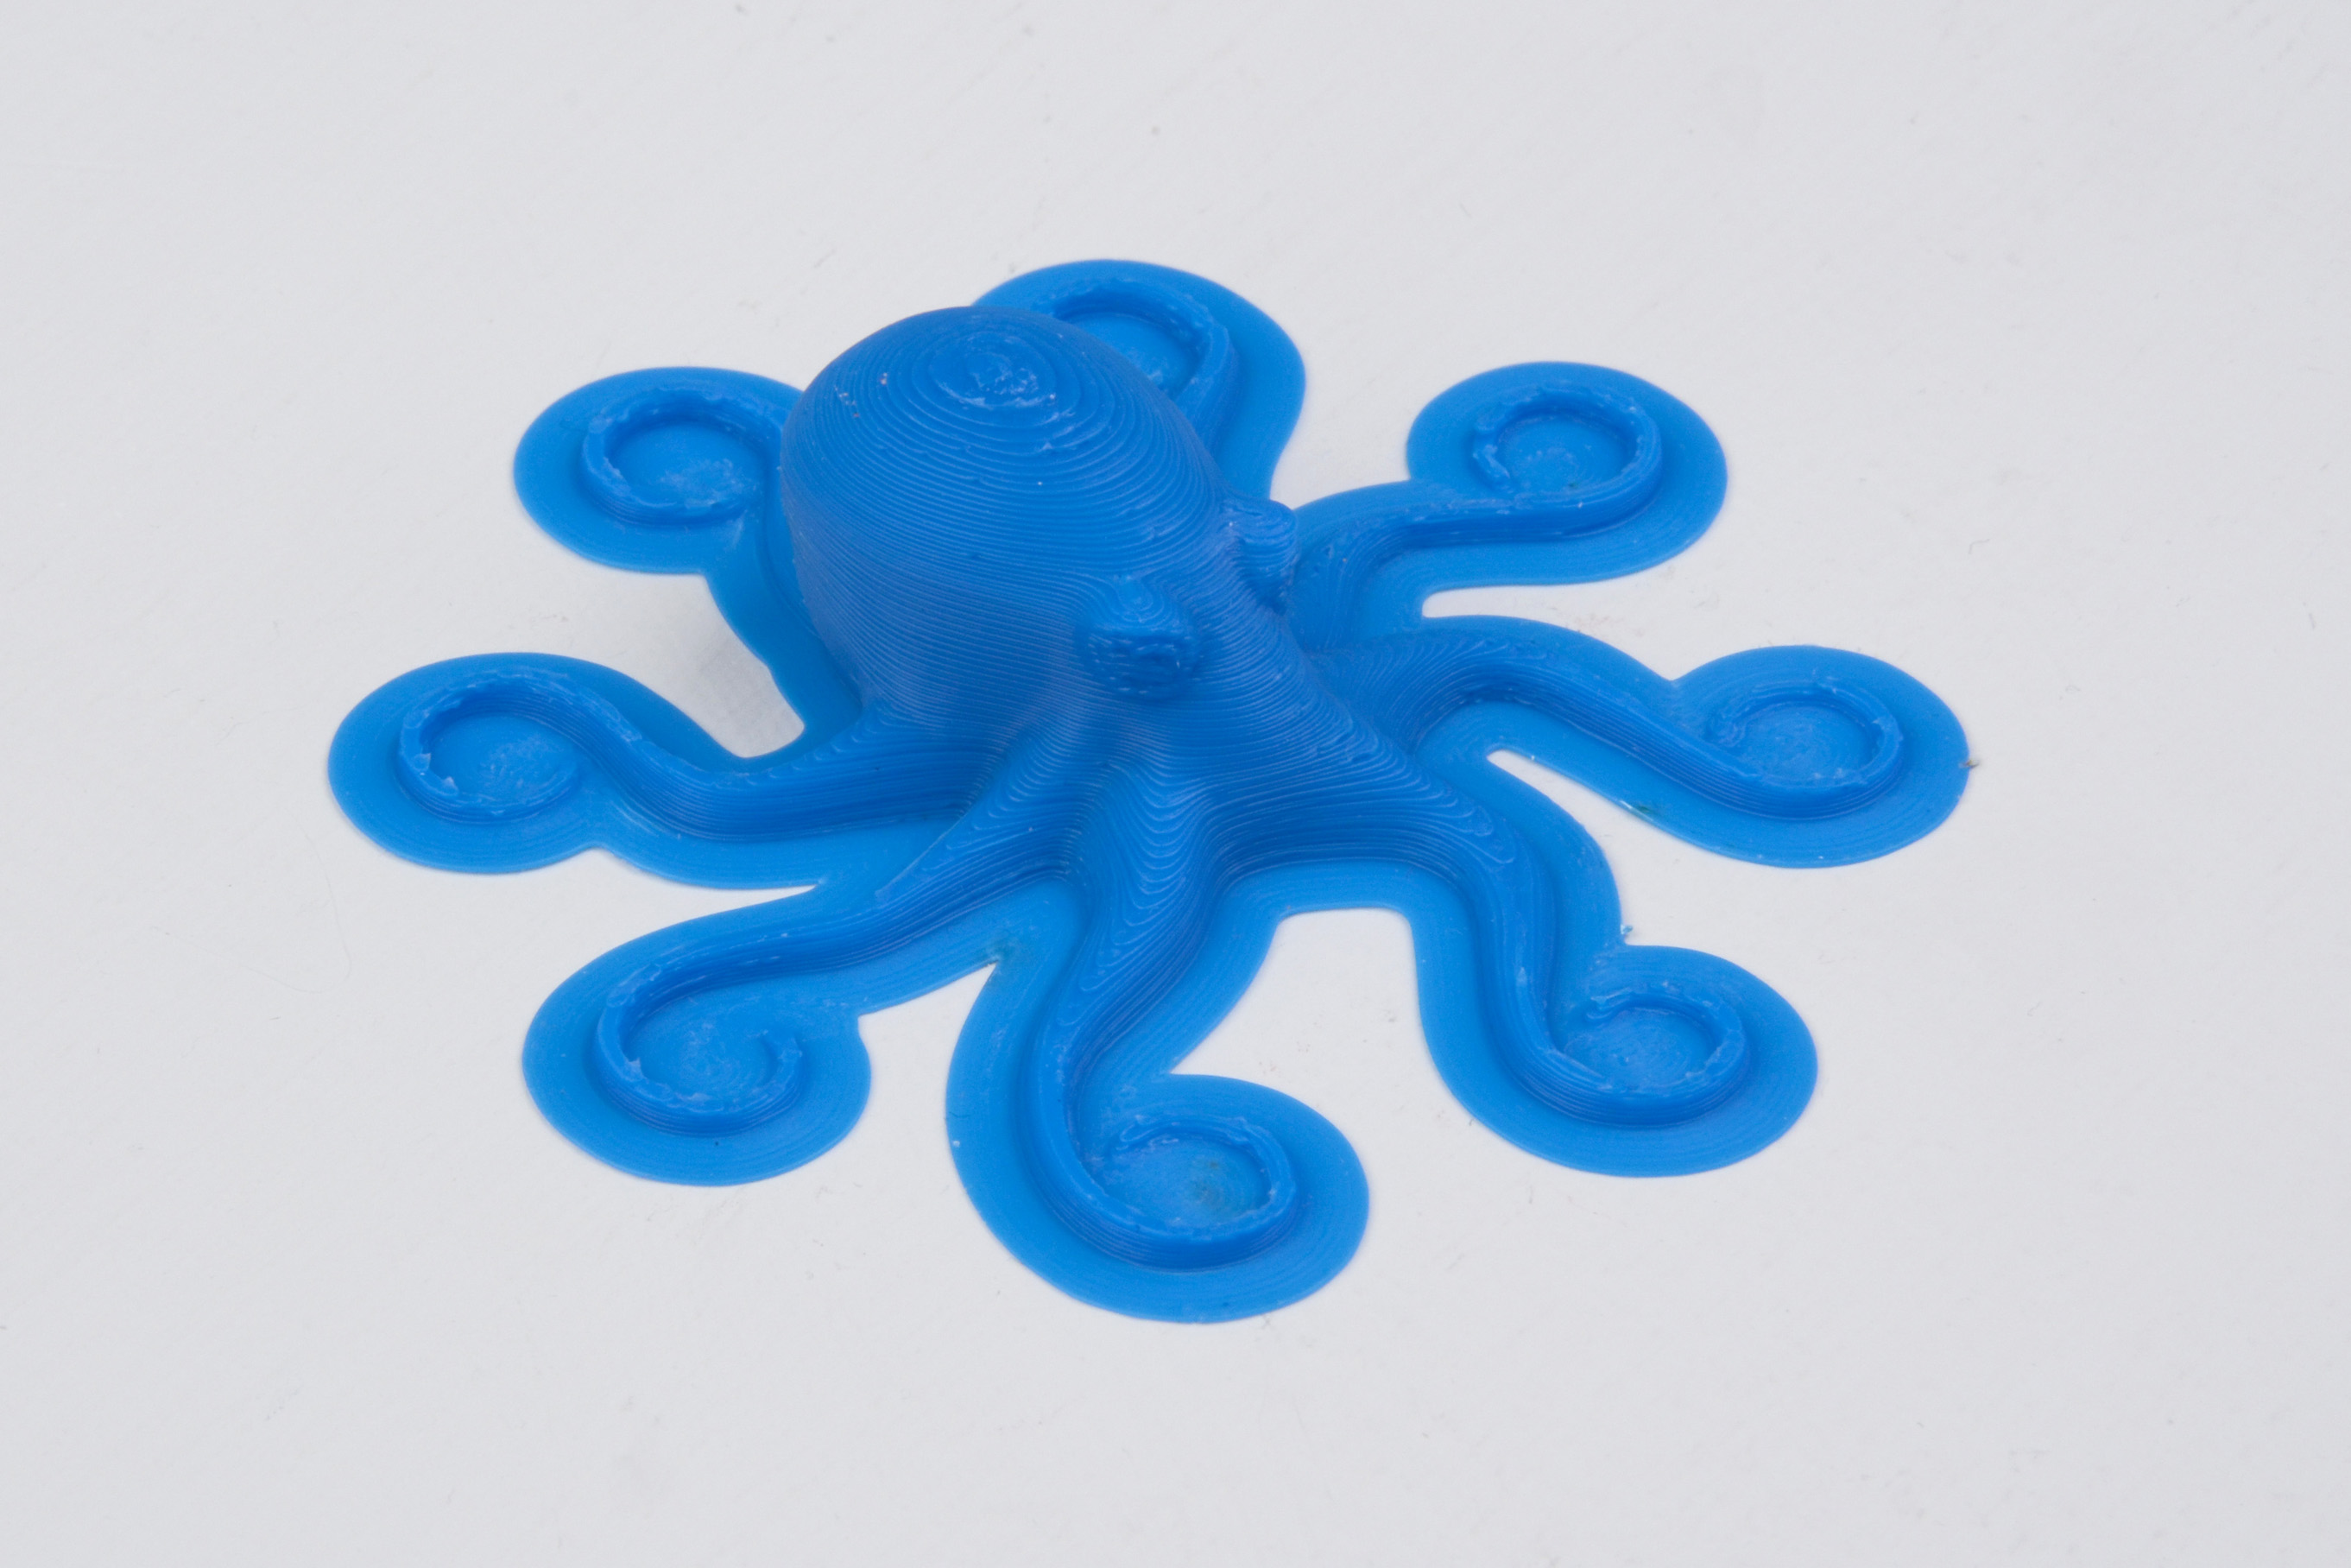
\includegraphics[keepaspectratio=true,width=0.75\textwidth]{simple_mode/brim.jpg}
\caption{An example of brim.}
\label{fig:an_example_of_brim}
\end{figure}

% paragraph brim (end)

\paragraph{Sequential Printing.} % (fold)
\label{par:sequential_printing}
This feature allows to compose a plate of objects but have the printer complete each one individually before going back to Z = 0 and starting with the next one. See the section about Sequential Printing in the Advanced Topics chapter.


\subsection{Filament Settings}
\index{Filament Settings}

The \texttt{Filament Settings} will normally be used infrequently, for example on receipt of a new roll of filament.

\begin{figure}[H]
\centering
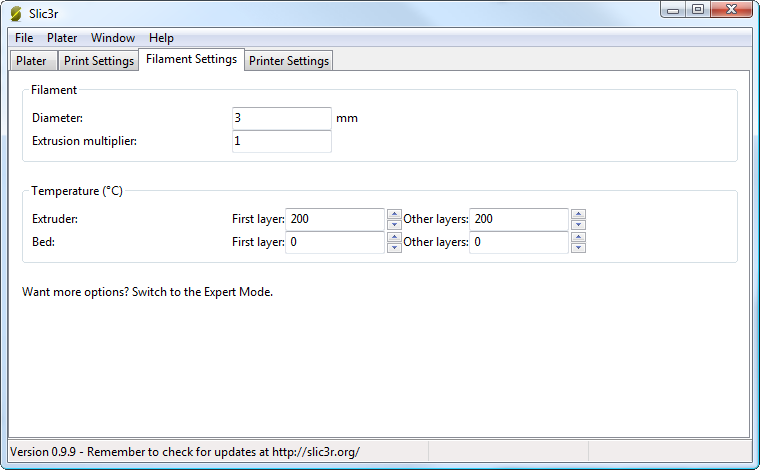
\includegraphics[width=\textwidth]{simple_mode/simple_mode_filament_settings.png}
\caption{Simple Mode: Filament Settings.}
\label{fig:simple_mode_filament_settings}
\end{figure}

\paragraph{Filament.} % (fold)
\label{par:filament}
\index{Filament Settings!Filament}
\index{Filament Settings!Filament!Diameter}
The \texttt{Diameter} setting will already have been filled from the value given during the wizard (see p.\pageref{sub:4_filament_diameter}), but can be updated here.

\index{Filament Settings!Filament!Extrusion multiplier}
The \texttt{Extrusion multiplier} setting allows the fine tuning of the extrusion flow rate, and is is given as a factor, e.g. 1 means 100\%, 1.5 would mean 150\%.  Whilst the value should ideally be set in the firmware it can be useful to test slight changes to the rate by altering this value.  It varies the amount of plastic proportionally and should be changed in very small steps (e.g. +/- 0.05) as the effects are very visible.
% paragraph filament (end)

\paragraph{Temperature.} % (fold)
\label{par:temperature}
\index{Filament Settings!Temperature!Extruder}
\index{Filament Settings!Temperature!Bed}
These values are also filled from the wizard, but here the opportunity exists to set the temperature for the first layer (see p.\pageref{sec:the_important_first_layer}).
% paragraph temperature (end)


\subsection{Printer Settings}
\index{Printer Settings}

The \texttt{Printer Settings} will be updated the least, unless Slic3r is going to be used for many printers, for example, in a 3D printer farm.

\begin{figure}[H]
\centering
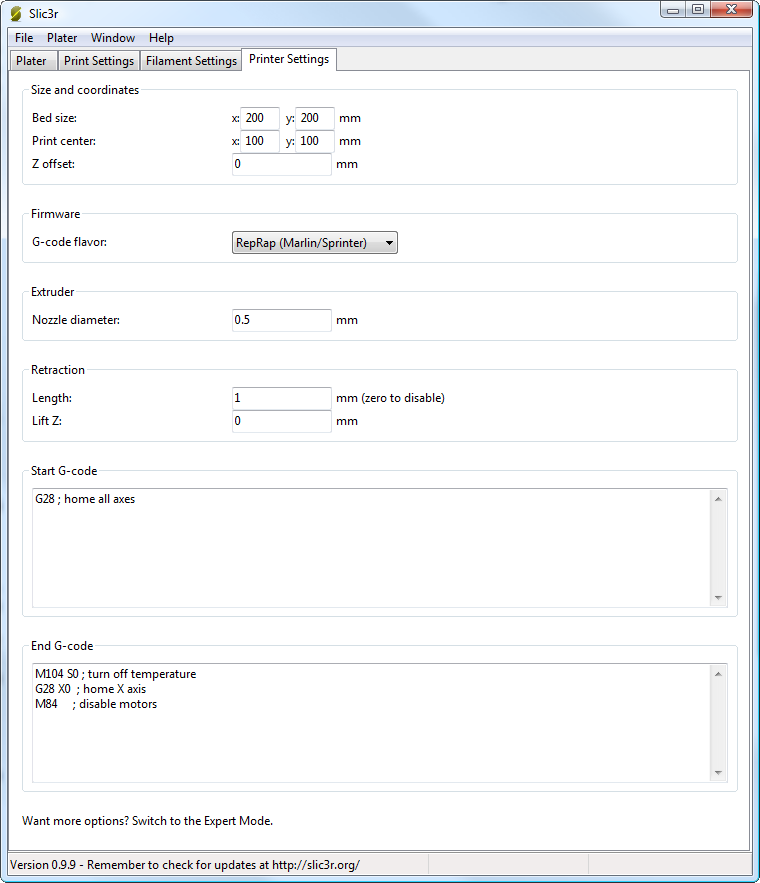
\includegraphics[width=\textwidth]{simple_mode/simple_mode_printer_settings.png}
\caption{Simple Mode: Printer Settings.}
\label{fig:simple_mode_printer_settings}
\end{figure}

\paragraph{Size and coordinates.} % (fold)
\label{par:size_and_coordinates}
\index{Printer Settings!Size and coordinates}
\index{Printer Settings!Size and coordinates!Bed size}
The \texttt{Bed size} setting is taken from the wizard (see p.\pageref{sub:2_bed_size}) and is only used for previewing the model in the plater.

\index{Printer Settings!Size and coordinates!Print center}
The \texttt{Print center} is the point around which the print will be centered.  A \texttt{Bed size} of 200mmx200mm and a \texttt{Print center} of 100mmx100mm would sit the print in the middle.  Should it be desired to print away from the center, because of a scratch in the glass perhaps, then this option should be used.

\index{Printer Settings!Size and coordinates!Z offset}
\texttt{Z offset} can be used to compensate for an incorrectly calibrated Z end-stop.  If the nozzle stops slightly too far from the bed, then adding a negative value will offset all layers by that amount.  The correct solution however is to fix the end-stop itself.

The optimal Z endstop position is where the nozzle tip barely touches the surface of the bed when homed.  A sheet of paper makes a good gauge for this very small distance.  It is not recommended to use this setting to try and improve layer adhesion, by "squashing" the bottom layer into the bed, instead look at the suggestions in section \ref{sec:the_important_first_layer}.
% paragraph size_and_coordinates (end)

\paragraph{Firmware.} % (fold)
\label{par:firmware}
\index{Printer Settings!Firmware!G-code flavour}
As selected in the wizard (see p.\pageref{sub:1_firmware_type}), \texttt{G-code flavour} defines the dialect of G-code generated.
% paragraph firmware (end)


\paragraph{Extruder.} % (fold)
\label{par:extruder}
\index{Printer Settings!Extruder!Nozzle diameter}
\texttt{Nozzle diameter} was defined in the wizard (see p.\pageref{sub:3_nozzle_diameter}).
% paragraph extruder (end)

\paragraph{Retraction.} % (fold)
\label{par:retraction}
\index{Printer Settings!Extruder!Retraction!Length}
Unless the material being extruded has a very high viscosity it may ooze between extrusions due to gravity.  This can be remedied by actively retracting the filament between extrusions.  Setting the \texttt{Length} parameter to a positive value will cause the filament to be reversed by that many millimeters before travel.  The retraction will then be compensated for by the same amount after the travel move, before starting the new extrusion path.

A value of between 1 and 2mm is usually recommended. Bowden extruders may need up to 4 or 5mm due to the hysteresis introduced by the tube.
\index{Printer Settings!Extruder!Retraction!Lift Z}
Setting the \texttt{Lift Z} parameter to a positive value will raise the entire extruder on the Z axis by that many millimeters during each travel.  This can be useful to ensure the nozzle will not catch on any already laid filament, however it is usually not necessary and will slow the print speed.  A value of 0.1mm is usually sufficient.
% paragraph retraction (end)

\paragraph{Start, End and Layer Chance G-codes.} % (fold)
\label{par:start_end_g_code}
\index{Printer Settings!Custom G-code!Start G-code}
\index{Printer Settings!Custom G-code!End G-code}
Custom G-code commands can be run before a print starts and after a print finishes.

Placeholders can be inserted in the G-code commands\footnote{https://github.com/alexrj/Slic3r/wiki/FAQ\#what-placeholders-can-i-use-in-custom-g-code}.  For example [next\_extruder] would return the index of the next extruder.

The RepRap wiki is a good resource to learn about the variety of G-codes available: \texttt{http://reprap.org/wiki/G-code}.

Note: Be sure to check that a given G-code is valid for your firmware.

The codes specified in \texttt{Start G-code} are inserted at the beginning of the output file, directly after the temperature control commands for extruder and bed.  Note that if temperature control commands are specified (M104 and M190) then these will replace the temperature G-codes introduced by the \texttt{Filament} settings.

Some common G-codes to use before the print starts are:
\begin{itemize}
	\item \textbf{G28}  - Homes all the axes.
\end{itemize}


Some common G-codes to use after the print ends are:
\begin{itemize}
	\item \textbf{M104 S0}  - Sets the extruder temperature to zero.
	\item \textbf{M140 S0} - Sets the heated bed temperature to zero.
	\item \textbf{G28 X0} - Home the X axis.
	\item \textbf{M84}  - Disables the motors.
\end{itemize}
% paragraph start_end_g_code (end)

% section simple_mode (end)\section{Simple Mode}
}
\fi
%%% END SIMPLE MODE %%%

%%% EXPERT MODE %%%
\ifadvanced
\chapter{\emph{Mode Expert}}
\thispagestyle{empty}
\markboth{Mode Expert}{Manuel Utilisateur de Slic3r}
{%!TEX root = Slic3r-Manual.tex

%!TEX root = Slic3r-Manual.tex

\section{Vitesse} % (fold)
\label{sec:speed}
\index{speed}
\index{vitesse}

Une fois que l'imprimante produit de manière fiable des impressions de bonne qualité, il peut être souhaitable d'augmenter la vitesse. Faire cela offre plusieurs avantages, le plus évident est que les résultats sont produits plus rapidement, mais aussi que le temps d'impression plus court peuvent être utilisés dans la production de plus de couches, pour la même hauteur de couche, améliorant ainsi la qualité d'impression perçue. Un avantage supplémentaire est qu'un mouvement plus rapide de déplacement entre les extrusions, peut réduire les effets de suintement.

La meilleure approche consiste à incrémenter les différents paramètres de vitesses par petites étapes et observer l'effet de chaque changement a sur la qualité d'impression. La vitesse de déplacement (travel speed) est un point de départ sur, et il n'est pas irréaliste d'atteindre des vitesses allant jusqu'à 250mm/s (si votre imprimante peut le gérer). Les réglages de la vitesse de périmètres (périmeters), de remplissage (infill) sont disponible en mode simple, et la règle générale est que le périmètre aille plus lentement que le remplissage afin de réduire les imperfections éventuelles sur la surface (remplissage peut être plus rapide parce que de légers défauts ne seront que importants).

Le Mode Expert offre plus de paramètres pour régler finement la vitesse de l'imprimante. La différenciation entre les périmètres extérieurs (external), petits (small) et d'autres périmètres, remplissage (infill), et les ponts (bridge)et les vide (gap) sont disponibles, ainsi que la capacité de ralentir la première couche.

\begin{figure}[H]
\centering
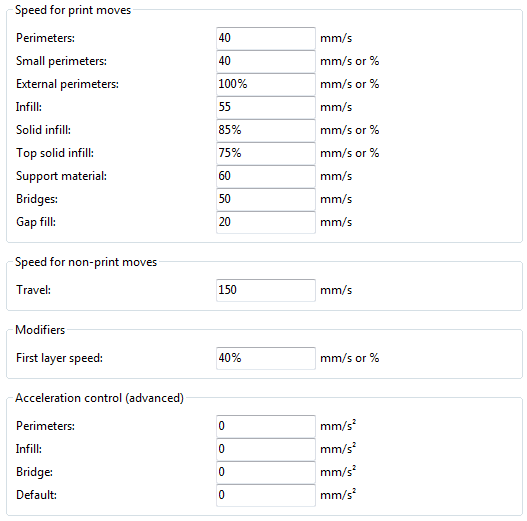
\includegraphics[keepaspectratio=true,width=1\textwidth]{expertmode/speed_advanced_settings.png}
\caption{Paramètres de vitesse en mode expert.}
\label{fig:speed_advanced_settings}
\end{figure}


Le cas échéant, une valeur peut être donnée en pourcentage. C'est par rapport à la valeur précédente, par exemple 50\% de remplissage solide sera la moitié de la valeur définie pour le remplissage.
\index{Print Settings!Speed}
\index{Paramètres d'Impression!Vitesse}
\index{Print Settings!Speed!Perimeters}
\index{Paramètres d'Impression!Vitesse!Périmètres}
\index{Print Settings!Speed!Small perimeters}
\index{Paramètres d'Impression!Vitesse!Périmètres courts}
\index{Print Settings!Speed!External perimeters}
\index{Paramètres d'Impression!Vitesse!Périmètres externes}
\index{Print Settings!Speed!Infill}
\index{Paramètres d'Impression!Vitesse!Remplissage}
\index{Print Settings!Speed!Solid infill}
\index{Paramètres d'Impression!Vitesse!Remplissage plein}
\index{Print Settings!Speed!Top solid }
\index{Paramètres d'Impression!Vitesse!Haut plein}
\index{Print Settings!Speed!Support material}
\index{Paramètres d'Impression!Vitesse!Support}
\index{Print Settings!Speed!Bridges}
\index{Paramètres d'Impression!Vitesse!Pont}
\index{Print Settings!Speed!Gap fill}
\index{Paramètres d'Impression!Vitesse!Remplissage des trous}
\index{Print Settings!Speed!Travel}
\index{Paramètres d'Impression!Vitesse!Déplacement}
\index{Print Settings!Speed!First layer speed}
\index{Paramètres d'Impression!Vitesse!Vitesse de la première couche}

Quelques directives générales pour chaque option:
\begin{itemize}
	\item \texttt{Perimeters} (périmètres) - En mode expert ce paramètre peut être légèrement suppérieur que le paramètre \texttt{External perimeters} (périmètres externes), peut être utilisé pour assurer les faces externes sans défaut.
	\item \texttt{Small perimeters} (petits périmètres) - Conçu pour les trous, les îles et les détails fins, une vitesse plus lente ici est recommandée.
	\item \texttt{External perimeters} (périmètres externes) - Une valeur légèrement plus lente peut assurer des surfaces propres.
	\item \texttt{Infill} (remplissage) - Aussi vite que vous le pouvez sans compromettre l'intégrité de la structure de remplissage. Les extrusions rapides peuvent se briser et entraîner des points faibles.
	\item \texttt{Solid infill} (remplissage solid) - L'extrusion pour le fond du modèle, et les couches solides supplémentaires est généralement un peu plus lente que le pour remplissage mais plus rapide que pour les périmètres.
	\item \texttt{Top solid infill} (remplissage solid du dessus) - Prévoyez du temps pour que l'extrusion couvre proprement les couches supérieures précédentes qu'elle aboutisse à une surface supérieure soigné. les dernières couches doivent parfaitement comblées la structure de remplissage, préparer la voie à une finition soignée.
	\item \texttt{Support material} (support) - Généralement les structures d'appui sont rapide et sale, et tant que que la base est correctement supportée, ils peuvent être construits aussi rapidement que possible.
	\item \texttt{Bridges} (ponts) - Obtenir une distance d'extrusion de portée dépend de la matière et du refroidissement. Aller trop lentement se traduira par l'affaissement, trop rapidement entraînera des brins cassés. L'expérimentation est ici la clé, mais généralement les pontages se réalise plus lentement que les périmètres.
	\item \texttt{Gap fill} (remplissage des vides) - Le remplissage de petits vides engendre de rapide oscillations de l'extrudeuse, la résultante des tremblements et résonance pourrait avoir un effet néfaste sur l'imprimante. Une valeur inférieure peut ici s'en prémunir cela. Un réglage à zéro désactive le remplissage de vide complètement.
	\item \texttt{Travel} (déplacement) - Aussi rapidement que votre imprimante permette afin de minimiser les suintements.
	\item \texttt{First layer speed} (vitesse de la 1ere couche) - Comme mentionné dans la section \ref{sec:the_important_first_layer}, fixer correctement la premère couche est important, et un rythme plus lent aide énormément. Définir un valeur de 50\%, voire moins, peut vraiment aider.
\end{itemize}

\index{Print Settings!Speed!Acceleration control}
\index{Paramètres d'Impression!Vitesse!Crontrole de l'accélération}
\texttt{Acceleration control} est un paramètre avancé permettant les paramètres d'accélération pour les périmètres, remplissage, pont, ainsi que d'un réglage par défaut, à faire. Décider quelles valeurs régler dépend des capacités de la machine. Tous les paramètres dans le firmware peuvent être un bon point de départ.

Tenir compte des restrictions imposées par le firmware comme beaucoup ont des paramètres de vitesse de sécurité maximale pour chaque axe.

% section speed (end)

\newpage

%!TEX root = Slic3r-Manual.tex

\section{Infill Patterns and Density} % (fold)
\label{sec:infill_patterns_and_density}
\index{infill}

There are several considerations when choosing an infill pattern: object strength, time and material, personal preference.  It can be inferred that a more complex pattern will require more moves, and hence take more time and material.
\index{Print Settings!Infill!Fill density}
\index{Print Settings!Infill!Fill pattern}
\index{Print Settings!Infill!Fill Top/bottom fill pattern}

\begin{figure}[H]
\centering
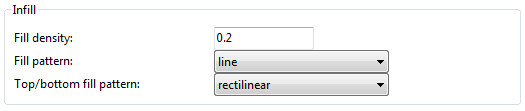
\includegraphics[keepaspectratio=true,width=1.0\textwidth]{expertmode/infill_pattern_settings.png}
\caption{Infill pattern settings.}
\label{fig:infill_pattern_settings}
\end{figure}

Slic3r offers several infill patterns, four regular, and three more exotic flavours.  The numbers given in brackets below each figure are a rough estimate of material used and time taken for a simple 20mm cube model\footnote{Taken from http://gcode.ws}.  Note that this is only indicative, as model complexity and other factors will affect time and material.

\begin{figure}[H]
\centering
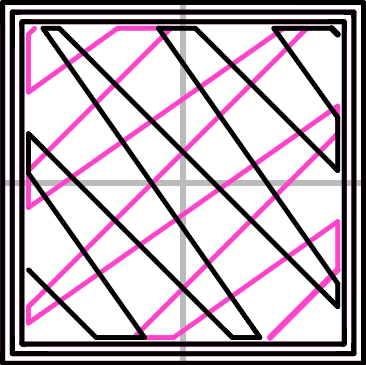
\includegraphics[keepaspectratio=true,width=0.2\textwidth]{expertmode/infill_line.png}
\caption{Infill pattern: Line (344.51mm / 5m:20s)}
\label{fig:infill_line}
\end{figure}

\begin{figure}[H]
\centering
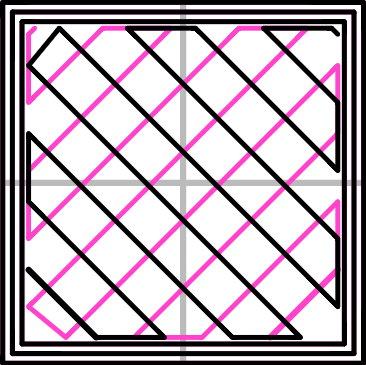
\includegraphics[keepaspectratio=true,width=0.2\textwidth]{expertmode/infill_rectilinear.png}
\caption{Infill pattern: Rectilinear (350.57mm / 5m:23s)}
\label{fig:infill_rectilinear}
\end{figure}

\begin{figure}[H]
\centering
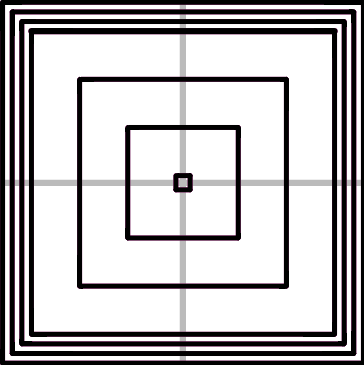
\includegraphics[keepaspectratio=true,width=0.2\textwidth]{expertmode/infill_concentric.png}
\caption{Infill pattern: Concentric (351.80mm / 5m:30s)}
\label{fig:infill_concentric}
\end{figure}

\begin{figure}[H]
\centering
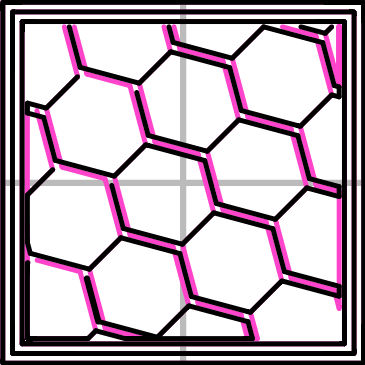
\includegraphics[keepaspectratio=true,width=0.2\textwidth]{expertmode/infill_honeycomb.png}
\caption{Infill pattern: Honeycomb (362.73mm / 5m:39s)}
\label{fig:infill_honeycomb}
\end{figure}

\begin{figure}[H]
\centering
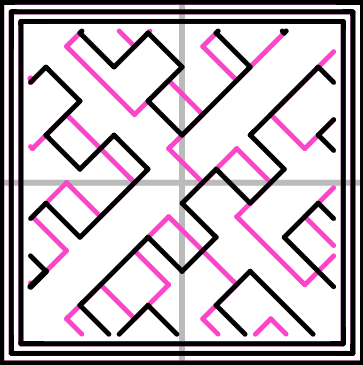
\includegraphics[keepaspectratio=true,width=0.2\textwidth]{expertmode/infill_hilbertcurve.png}
\caption{Infill pattern: Hilbert Curve (332.82mm / 5m:28s)}
\label{fig:infill_hilbertcurve}
\end{figure}

\begin{figure}[H]
\centering
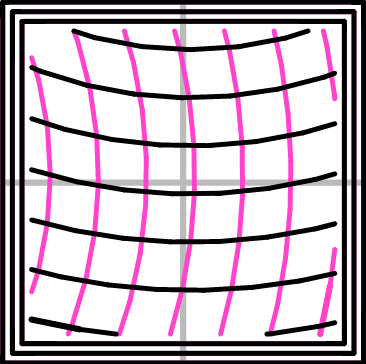
\includegraphics[keepaspectratio=true,width=0.2\textwidth]{expertmode/infill_archimedeanchords.png}
\caption{Infill pattern: Archimedean Chords (333.66mm / 5m:27s)}
\label{fig:infill_archimedeanchords}
\end{figure}

\begin{figure}[H]
\centering
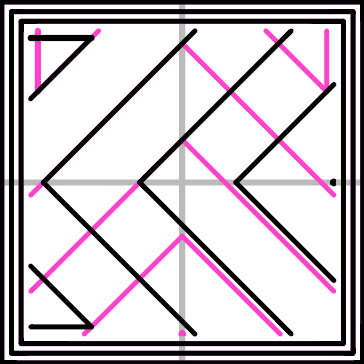
\includegraphics[keepaspectratio=true,width=0.2\textwidth]{expertmode/infill_octagramspiral.png}
\caption{Infill pattern: Octagram Spiral (318.63mm / 5m:15s)}
\label{fig:infill_octagramspiral}
\end{figure}


Certain model types are more suited for a particular pattern, for example organic versus mechanical types.  Figure \ref{fig:complex_object_infill_comparison} shows how a honeycomb fill may suit this mechanical part better because each hexagon bonds with the same underlying pattern each layer, forming a strong vertical structure.

\begin{figure}[H]
\centering
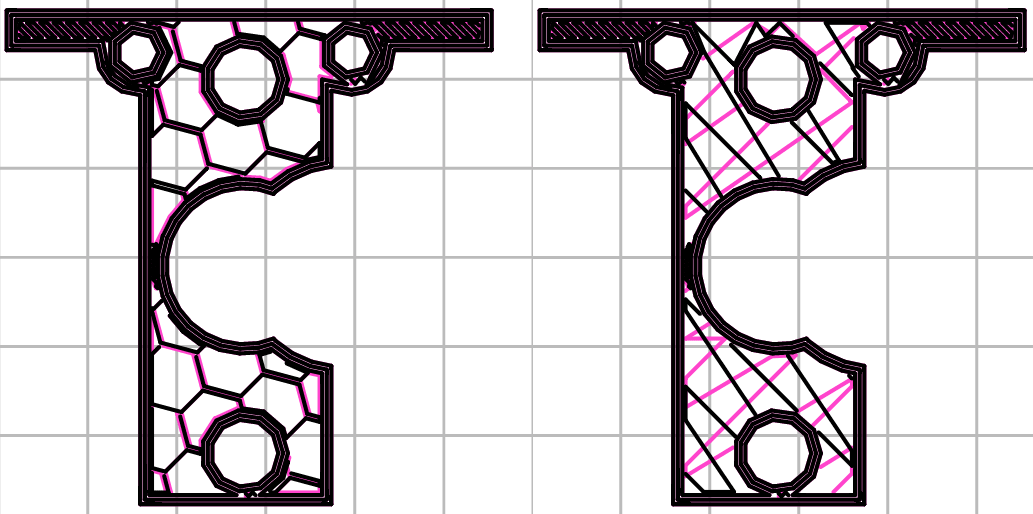
\includegraphics[keepaspectratio=true,width=0.75\textwidth]{expertmode/complex_object_infill_comparison.png}
\caption{Infill pattern comparison in a complex object. Left to Right: honeycomb, line}
\label{fig:complex_object_infill_comparison}
\end{figure}

Most models require only a low density infill, as providing more than, say, 50\% will produce a very tightly packed model which uses more material than required.  For this reason a common range of patterns is between 10\% and 30\%, however the requirements of the model will determine which density is best.  Figure \ref{fig:infill_pattern_densities} shows how the patterns change as the density increases.
\begin{figure}[H]
\centering
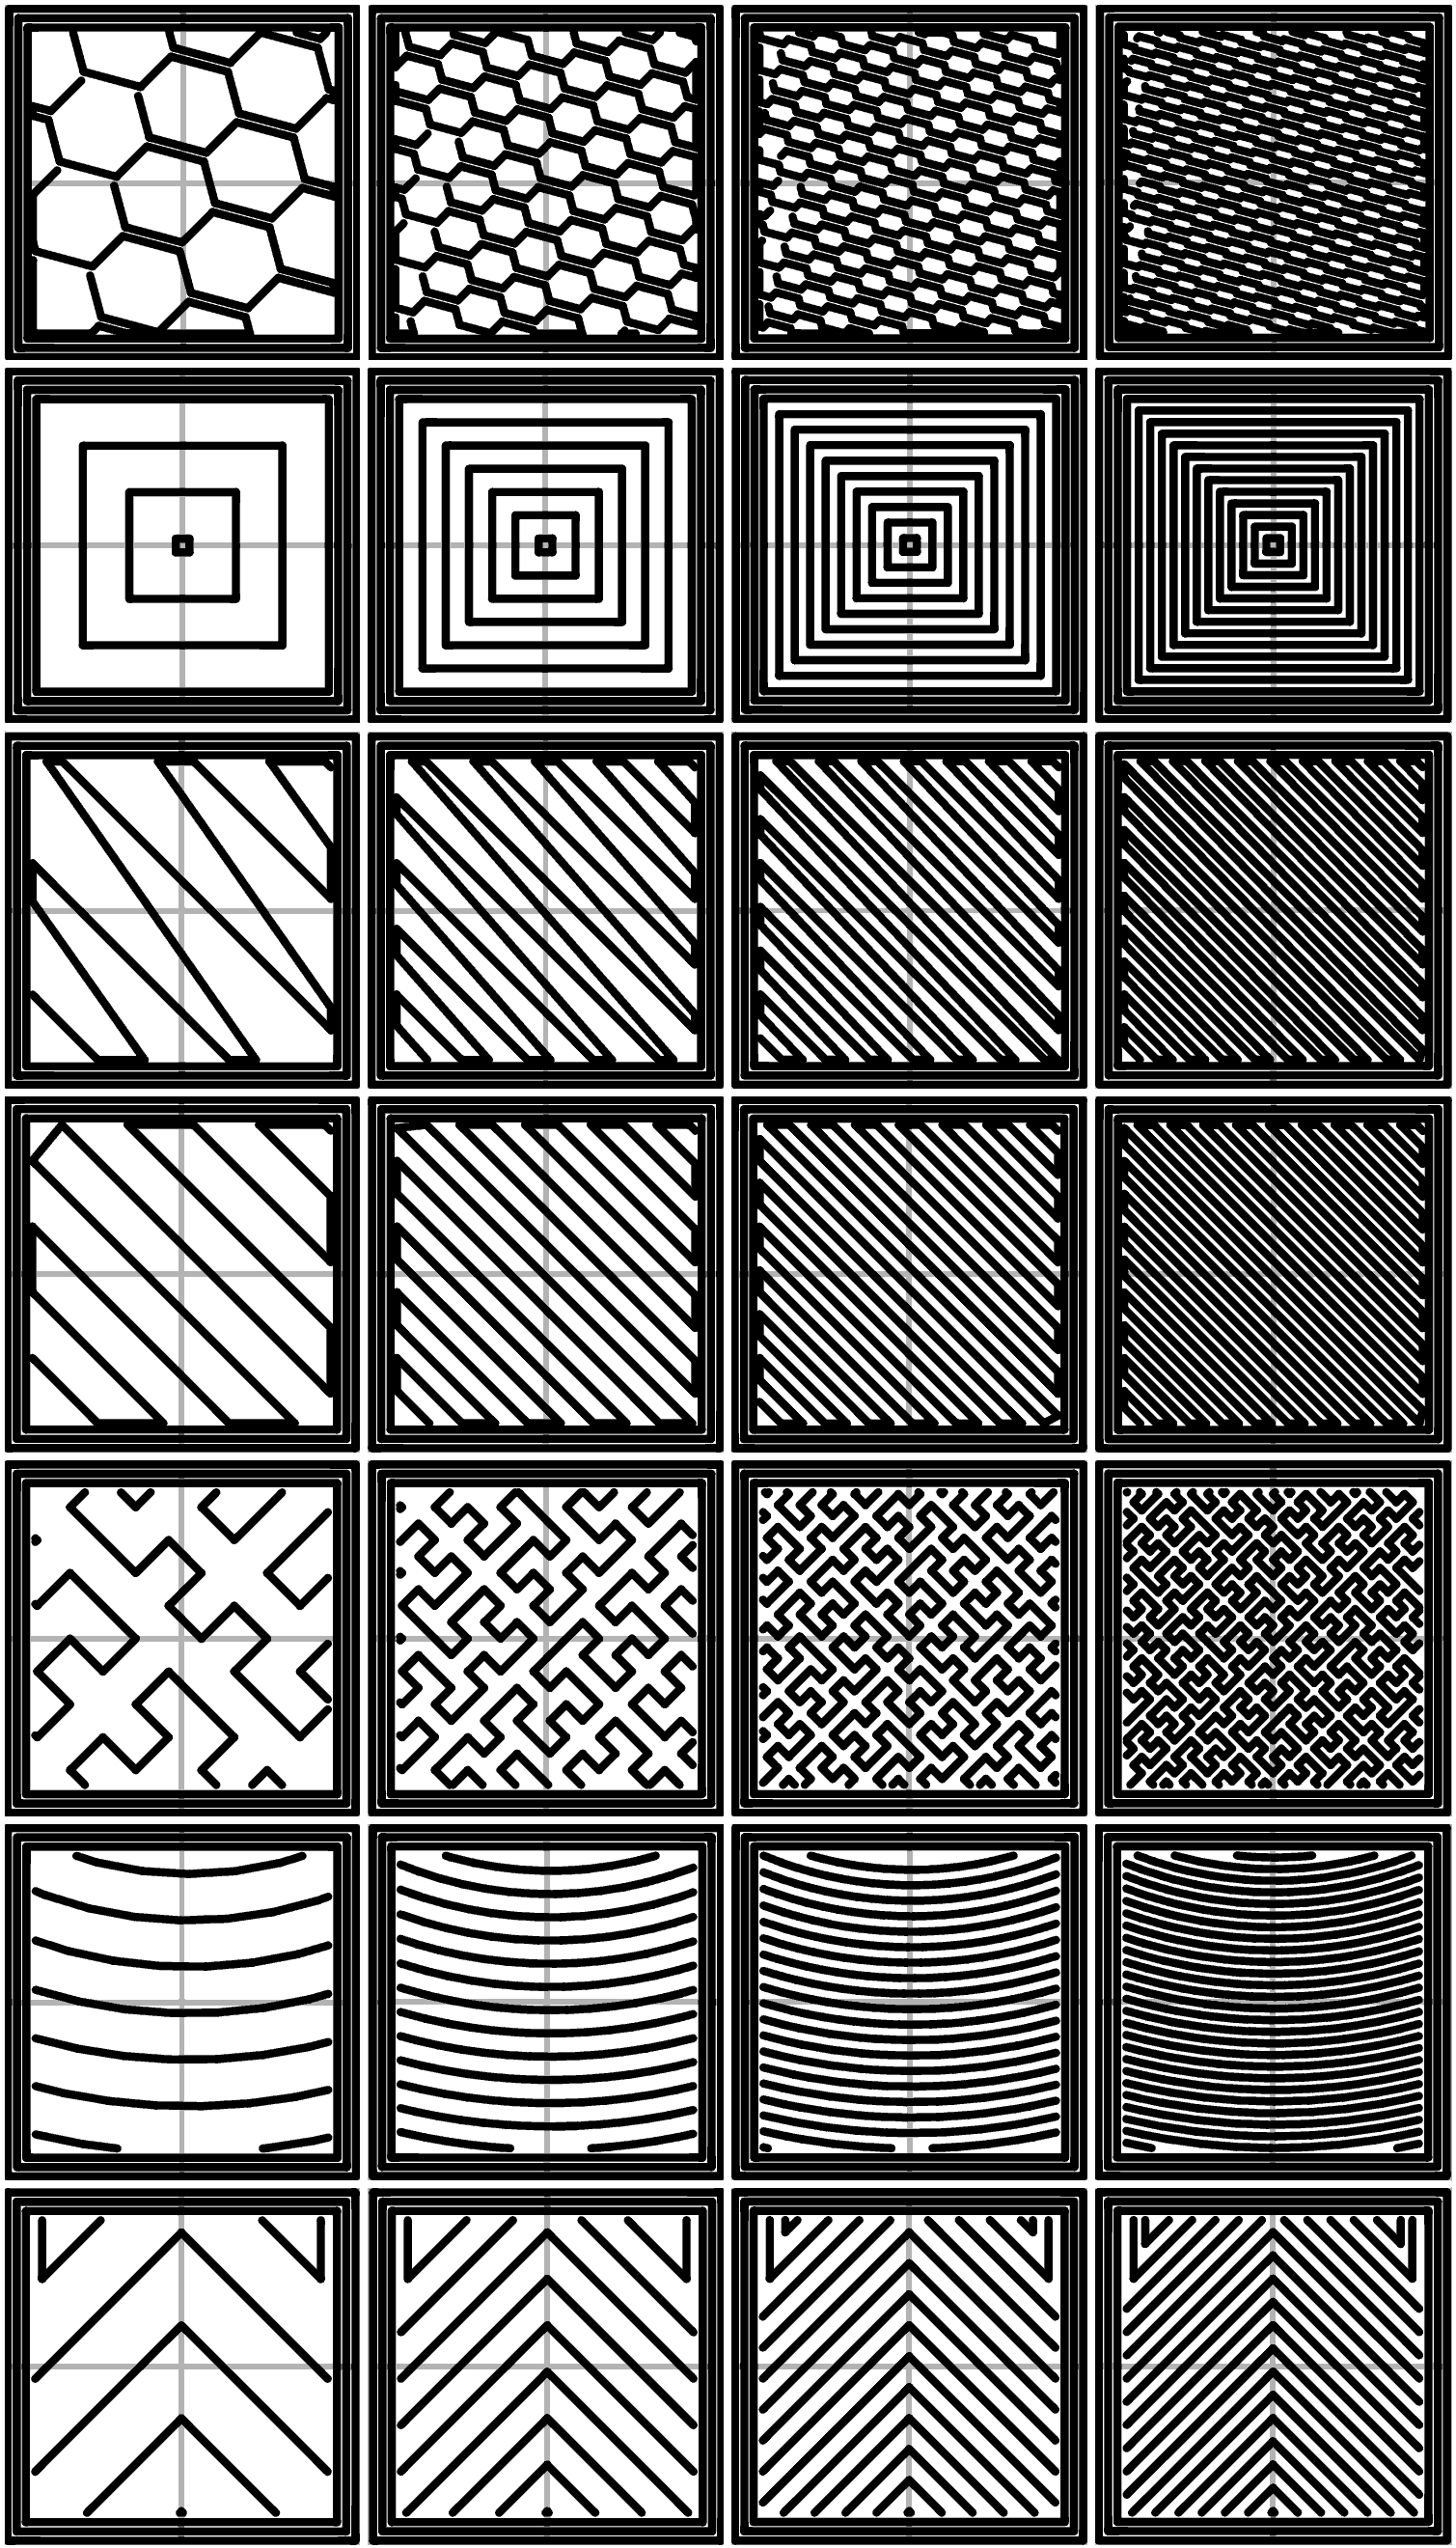
\includegraphics[keepaspectratio=true,width=0.7\textwidth]{expertmode/infills.png}
\caption{Infill patterns at varying densities. Left to Right: 20\%,40\%,60\%,80\%. Top to Bottom: Honeycomb, Concentric, Line, Rectilinear, Hilbert Curve, Archimedean Chords, Octagram Spiral}
\label{fig:infill_pattern_densities}
\end{figure}

% section infill_patterns_and_density (end)

\newpage

%!TEX root = Slic3r-Manual.tex

\section{Infill Optimization} % (fold)
\label{sec:infill_optimization}
\index{infill}

Slic3r contains several advanced infill settings which can help produce better extrusions.

\begin{figure}[H]
\centering
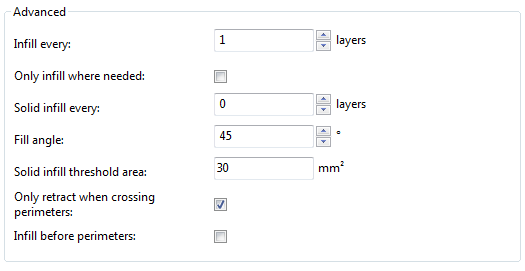
\includegraphics[keepaspectratio=true,width=1\textwidth]{expertmode/infill_advanced_settings.png}
\caption{Infill advanced settings.}
\label{fig:infill_settings}
\end{figure}
\index{Print Settings!Infill!Infill every n layers}
\index{Print Settings!Infill!Only infill where needed}
\index{Print Settings!Infill!Solid infill every n layers}
\index{Print Settings!Infill!Fill angle}
\index{Print Settings!Infill!Solid infill threshold area}
\index{Print Settings!Infill!Only retract when crossing perimeters}
\index{Print Settings!Infill!Infill before perimeters}

\begin{itemize}
    \item \texttt{Infill every \textit{n} layers} - Will produce sparse vertical infill by skipping a set number of layers. This can be used to speed up print times where the missing infill is acceptable.
    \item \texttt{Only infill where needed} - Slic3r will analyse the model and choose where infill is required in order to support internal ceilings and overhangs.  Useful for reducing time and materials.
    \item \texttt{Solid infill every \textit{n} layers} - Forces a solid fill pattern on the specified layers.  Zero will disable this option.
    \item \texttt{Fill angle} - By default the infill pattern runs at 45° to the model to provide the best adhesion to wall structures.  Infill extrusions that run adjacent to perimeters are liable to de-laminate under stress.  Some models may benefit from rotating the fill angle to ensure the optimal direction of the extrusion.
    \item \texttt{Solid infill threshold area} - Small areas within the model are usually best off being filled completely to provide structural integrity.  This will however take more time and material, and can result in parts being unnecessarily solid.  Adjust this option to balance these needs.
    \item \texttt{Only retract when crossing perimeters} - Retracting, to prevent ooze, is unnecessary if the extruder remains within the boundaries of the model.  Care should be taken if the print material oozes excessively, as not retracting may result in enough material loss to affect the quality of the subsequent extrusion.  However, most modern printers and materials rarely suffer from such extreme ooze problems.
    \item \texttt{Infill before perimeters} - Reverses the order in which the layer is printed. Usually the perimeter is laid down initially, followed by the infill, and this is usually the preferable as the perimeter acts as a wall containing the infill.
\end{itemize}


% section infill_optimization (end)

\newpage

%!TEX root = Slic3r-Manual.tex

\section{Fighting Ooze} % (fold)
\label{sec:fighting_ooze}
\index{ooze}
\index{retraction}

Unless the material being extruded has a very high viscosity it will ooze from the nozzle in between extrusions.  There are several settings in Slic3r to which can help to remedy this.

The retraction settings, found in the \texttt{Printer} tab, tell the printer to pull back the filament between extrusion moves.  This can alleviate the pressure in the nozzle, thus reducing ooze.  After the subsequent travel move the retraction is reversed to prepare the extruder for the next extrusion.

\begin{figure}[H]
\centering
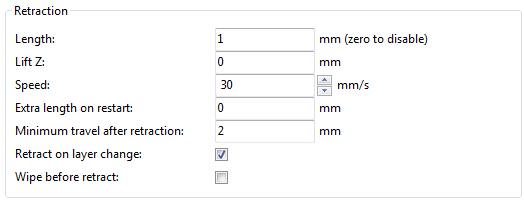
\includegraphics[keepaspectratio=true,width=1.0\textwidth]{expertmode/retraction_settings.png}
\caption{Retraction settings.}
\label{fig:retraction_settings}
\end{figure}
\index{Printer Settings!Extruder!Retraction!Length}
\index{Printer Settings!Extruder!Retraction!Lift Z}
\index{Printer Settings!Extruder!Retraction!Speed}
\index{Printer Settings!Extruder!Retraction!Extra length on restart}
\index{Printer Settings!Extruder!Retraction!Minimum travel after retraction}
\index{Printer Settings!Extruder!Retraction!Retract on layer change}
\index{Printer Settings!Extruder!Retraction!Wipe before retract}

\begin{itemize}
    \item \texttt{Length} - The number of millimeters to retract.  Note that the measurement is taken from the raw filament entering the extruder.  A value of between 1 and 2mm is usually recommended. Bowden extruders may need up to 4 or 5mm due to the hysteresis introduced by the tube.
    \item \texttt{Lift Z} - Raises the entire extruder on the Z axis by that many millimeters during each travel.  This can be useful to ensure the nozzle will not catch on any already laid filament, however it is usually not necessary and will slow the print speed.  A value of 0.1mm is usually sufficient.
    \item \texttt{Speed} - The speed at which the extruder motor will pull back the filament.  The value should be set to as quick as the extruder can handle without skipping steps, and it is worth experimenting with this value to find the quickest retraction possible.
    \item \texttt{Extra length on restart} -  Adds an extra length of filament after the retraction is compensated after the travel move. This setting is rarely used, however should the print show signs of not having enough material after travel moves then it may be useful to add a small amount of additional material.
    \item \texttt{Minimum travel after retraction} - Triggering a retraction after very short moves is usually unnecessary as the amount of ooze is usually insignificant and it slows down the print times.  Set the number of millimeters minimum distance the nozzle must move before considering a retraction.  If the printer handles ooze well this can be increased to 5 or 6mm.
    \item \texttt{Retract on layer change} - Movement along the Z axis must also be considered when dealing with oozing, otherwise blobs may occur.  It is recommended to leave this setting on.
    \item \texttt{Wipe before retract} - Moves the nozzle whilst retracting so as to reduce the chances of a blob forming.
\end{itemize}


Additionally there are several settings in the \texttt{Print} tab which can help control oozing.

\begin{itemize}
    \index{Print Settings!Infill!Only retract when crossing perimeters}
    \item \texttt{Only retract when crossing perimeters} (Infill) - Tells Slic3r to only retract if the nozzle will cross the threshold of the current island being extruded.  Slight ooze within the walls of a part are not seen and can usually be accepted.
    \index{Print Settings!Layers and perimeters!Advanced!Avoid crossing perimeters}
    \item \texttt{Avoid crossing perimeters} (Layers and perimeters - Advanced) - Will force the nozzle to follow perimeters as much as possible to minimise the number of times it must cross them when moving around, and between, islands.  This has a negative impact on both G-code generation and print times.
    \index{Print Settings!Layers and perimeters!Vertical shells!Randomize starting points}
    \item \texttt{Randomize starting points} (Layers and perimeters - Vertical shells) - As the extruder moves up to the start of the next layer any ooze can result in blobs.  If the same start point is used for every layer then a seam can form the length of the object.  This setting will move the start point to a difference location for each layer.
\end{itemize}


See also section \ref{par:simple_sequential_printing}: Sequential Printing for another technique which can minimise strings forming between objects.
% section fighting_ooze (end)

\newpage

%!TEX root = Slic3r-Manual.tex

\section{Skirt} % (fold)
\label{sec:skirt}
\index{skirt}
\index{Print Settings!Skirt and brim!Skirt}

The \texttt{Skirt} setting adds an extrusion a short distance away from the perimiter of the object.  This can ensure that the material is flowing smoothly from the extruder before it starts on the model proper.

\begin{figure}[H]
\centering
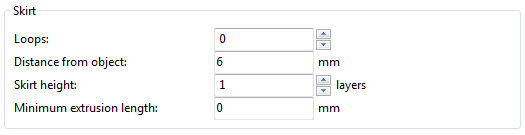
\includegraphics[keepaspectratio=true,width=1.0\textwidth]{expertmode/skirt_settings.png}
\caption{Skirt settings.}
\label{fig:skirt_settings}
\end{figure}

\begin{itemize}
    \index{Print Settings!Skirt and brim!Skirt!Loops}
    \item \texttt{Loops} - How many circuits should be completed before starting on the model.  One loop is usually sufficient.
    \index{Print Settings!Skirt and brim!Skirt!Distance from object}
    \item \texttt{Distance from object} - The millimeters between the object and the skirt.  The default of 6mm is usually sufficient.
    \index{Print Settings!Skirt and brim!Skirt!Skirt height}
    \item \texttt{Skirt height} - The number of layers to lay down a skirt for.  For ensuring the material is flowing smoothly, one layer is sufficient, however the skirt function can also be used to build walls around the object in case it should be protected from draughts.
    \index{Print Settings!Skirt and brim!Skirt!Minimum extrusion length}
    \item \texttt{Minimum extrusion length} - Dictates a minimum number of millimeters that the skirt should be, should the loop around the object not be enough.
\end{itemize}

% section skirt (end)

\newpage

%!TEX root = Slic3r-Manual.tex

\section{Cooling} % (fold)
\label{sec:cooling}
\index{cooling}
\index{temperature}

Temperature plays a key part in determining print quality.  Too hot and the material deforms, too cool and layer adhesion may be problematic.  Applying cooling will allow the freshly deposited material to solidify enough to provide a good base for the next layer, helping with overhangs, small details and bridges.

There are two main techniques for cooling: adding a fan and slowing down the print speed.  Slic3r may choose to use both techniques, using a fan first, and then slowing down the print if the layer time is too fast.

\begin{figure}[H]
\centering
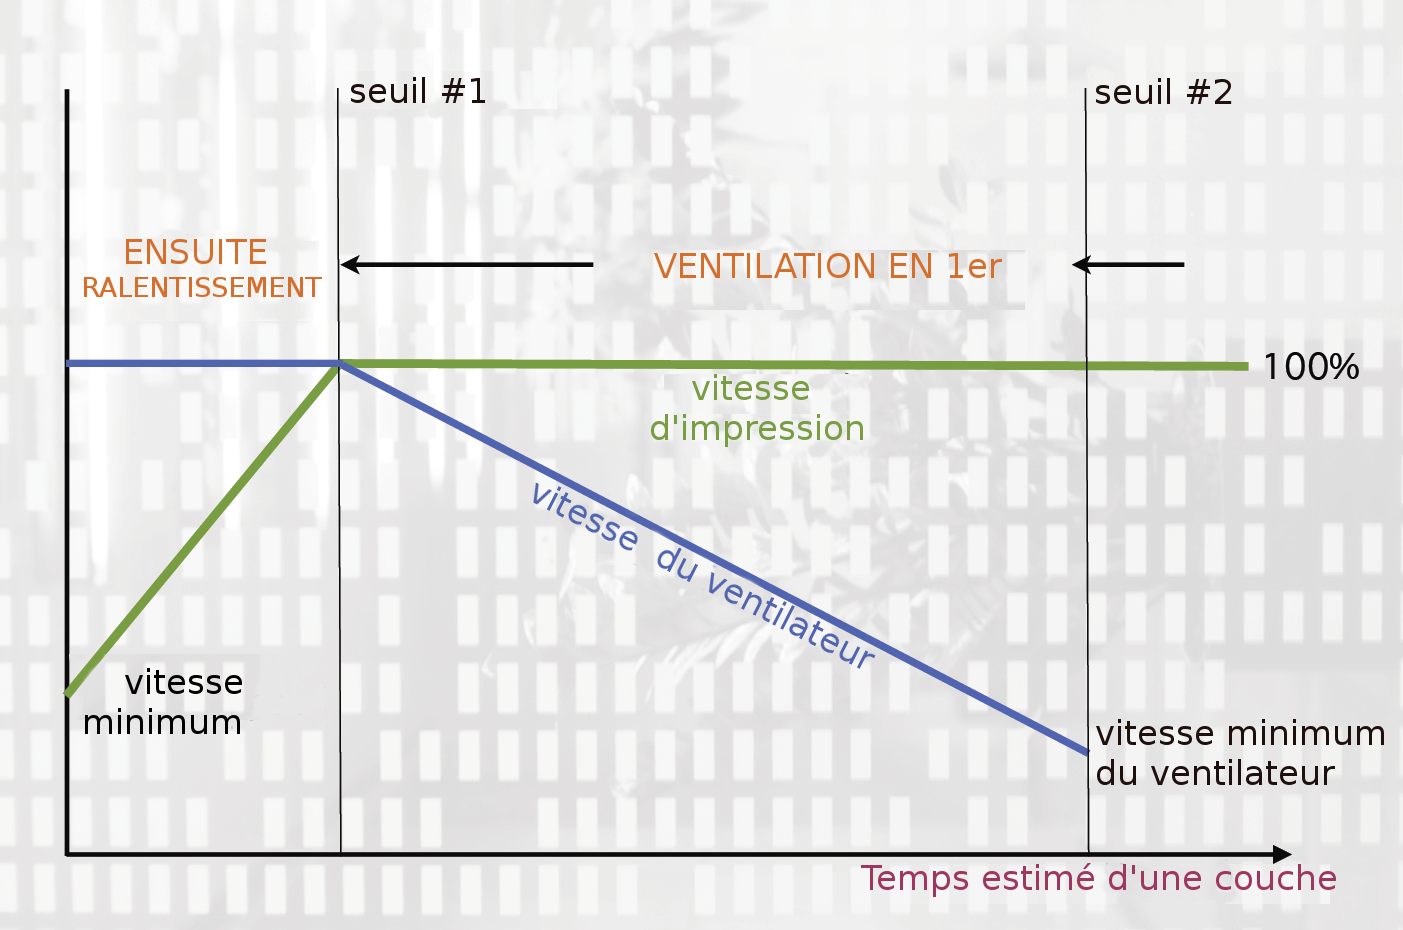
\includegraphics[keepaspectratio=true,width=1\textwidth]{expertmode/cooling_chart.png}
\caption{Cooling strategy.}
\label{fig:cooling_chart}
\end{figure}

Figure \ref{fig:cooling_chart} shows the strategy adopted by Slic3r.  Reading from right to left, when the minimum fan threshold (\#2) is reached the fan is turned on.  This increases in intensity as the layer time decreases.  The print speed remains constant until the estimated print time drops below a certain threshold (\#1), this is when the print speed is reduced until it reaches it's minimum value.

\subsection{Fans} % (fold)
\label{sub:fans}
\index{cooling!fans}
Most electronics and firmware allow the addition of a fan via a spare connector.  These can then be instructed with G-code, from Slic3r, to turn on or off as the model requires, and to rotate at different speeds.

Care should be taken with the positioning of the fan so that it does not cool any heated bed more than necessary.  It should also not cool the heater block of the hot-end so as not to force it to do more work and waste energy.  The air movement should aim for the nozzle tip, flowing over the freshly extruded material.

A duct may help in guiding the flow correctly, and there are several designs available online, for a wide variety of printers.

% subsection fans (end)

\subsection{Slowing Down} % (fold)
\label{sub:slowing_down}
\index{cooling!slowing down}
Slic3r can tell the printer to slow down if the estimated layer time is above a certain threshold.

Care must be taken as the intended effect could be mitigated by the nozzle not moving far enough away from the fresh extrusion, a problem with small, detailed layers.  For this reason it is usually recommended to use a fan where possible.
% subsection slowing_down (end)

\subsection{Configuring} % (fold)
\label{sub:configuring_cooling}

In simple mode Slic3r will attempt to choose the optimal settings for both fans and speed.  Expert mode gives more granular options.

\begin{figure}[H]
\centering
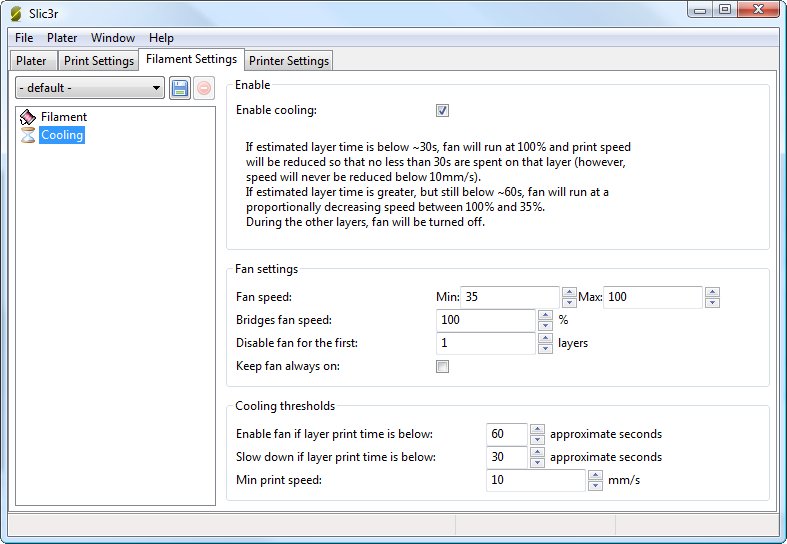
\includegraphics[keepaspectratio=true,width=1\textwidth]{expertmode/cooling_advanced_settings.png}
\caption{Cooling advanced settings.}
\label{fig:cooling_advanced_settings}
\end{figure}

\begin{itemize}
    \index{Filament Settings!Cooling!Fan speed}
	\item \texttt{Fan speed}  - Determines the minimum and maximum speeds - useful for fans that run too fast by default.
    \index{Filament Settings!Cooling!Bridges fan speed}
	\item \texttt{Bridges fan speed}  - As the material stretches over wide gaps, it makes sense to try and cool it as much as possible, therefore a full fan speed is recommended.
    \index{Filament Settings!Cooling!Disable fan for first n layers}
	\item \texttt{Disable fan for first \textit{n} layers}  - Section \ref{sec:the_important_first_layer} detailed how important the first layer is, and so it makes sense not to apply the fan until sure the print is securely attached to the bed.  Keeping the fan turned off for the first two or three layers is a good idea.
    \index{Filament Settings!Cooling!Keep fan always on}
	\item \texttt{Keep fan always on}  - Overrides any other choices and has the fan run continuously, at least at the minimum speed setting.  This can be useful when printing with PLA, but is not recommended for ABS.
\end{itemize}

\begin{itemize}
    \index{Filament Settings!Cooling!Enable fan if print time is below t seconds}
	\item \texttt{Enable fan if print time is below \textit{t} seconds}  - Triggers the fan if the layer will be completed within the given number of seconds.
    \index{Filament Settings!Cooling!Slow down if layer print time is below t seconds}
	\item \texttt{Slow down if layer print time is below \textit{t} seconds}  - Slows down the print if the layer will be completed within the given number of seconds.
    \index{Filament Settings!Cooling!Min print speed}
	\item \texttt{Min print speed}  - A lower limit on how slowly a layer can be printed.
\end{itemize}


% subsection configuring_cooling (end)

% section cooling (end)

\newpage

%!TEX root = Slic3r-Manual.tex
\section{Mati\`ere de Support} % (fold)
\label{sec:support}
\index{support material}
\index{mati\`ere de support}

En g\'en\'eral, la plupart des mod\`eles 3D seront imprim\'ees avec des parties en surplomb jusqu'\`a une certaine inclinaison. L'angle est d\'etermin\'e par plusieurs facteurs, notamment la hauteur de la couche et la largeur d'extrusion, et est g\'en\'eralement autour de 45 °. Pour les mod\`eles avec de plus grands surplombs une structure de support peut \^etre imprim\'e en dessous. Cela engage l'utilisation de plus de mati\`ere, plus le temps d'impression, et un nettoyage apr\`es l'impression.

\begin{figure}[H]
\centering
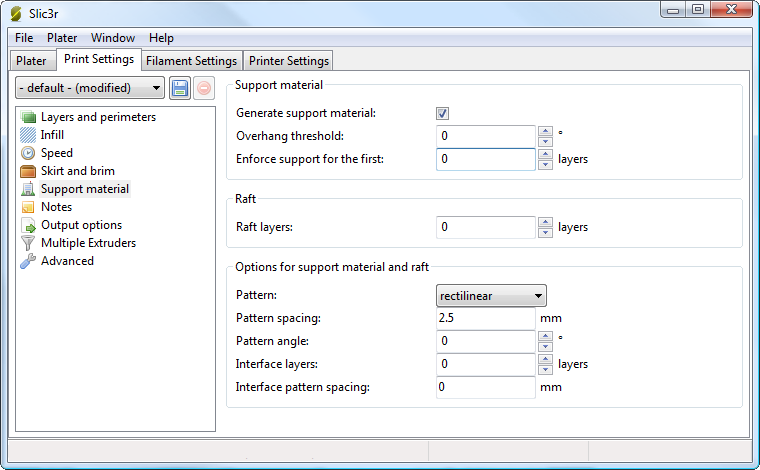
\includegraphics[keepaspectratio=true,width=1\textwidth]{expertmode/support/advanced_support.png}
\caption{Param\`etres de support.}
\label{fig:advanced_support}
\end{figure}
\index{Print Settings!Support material!Generate support material}
\index{Param\`etres d'Impression!Mati\`ere de Support!G\'en\'erer un support}
\index{Print Settings!Support material!Overhang threshold}
\index{Param\`etres d'Impression!Mati\`ere de Support!Seuil de porte \`a faux}
\index{Print Settings!Support material!Enforce support}
\index{Param\`etres d'Impression!Mati\`ere de Support!Appliquer le support}

La premi\`ere chose \`a faire est d'activer l'option de mati\`ere de support en cochant la case \texttt{Generate support material} (G\'en\'erer un support).  Mettre \`a z\'ero le param\`etre \texttt{Overhang threshold} (Seuil de porte \`a faux) indique \`a Slic3r de d\'etecter les lieux o\`u apporter un soutien automatiquement, sinon l'angle indiqu\'e sera utilis\'e.  La g\'en\'eration de support est un sujet relativement complexe, et il ya plusieurs aspects qui d\'eterminent le soutien optimal, il est fortement recommand\'e de fixer le seuil \`a z\'ero et permettre Slic3r de d\'eterminer le soutien n\'ecessaire.

Les petits mod\`eles, et ceux avec de petites empreintes \`a la base, peuvent parfois se briser ou se d\'etacher du lit.  Pour cette raison le param\`etre \texttt{Enforce support} (Appliquer le support) produira des structures de support \`a imprimer pour le nombre donn\'e de couches, ind\'ependamment de la valeur de seuil d'angle.

Pour d\'emontrer les modes de remplissage le mod\`ele minimug a \'et\'e inclin\'e de 45 ° le long de l'axe x, comme repr\'esent\'e sur la figure \ref{fig:support_minimug_45deg}.
\index{Print Settings!Support material!Pattern}
\index{Param\`etres d'Impression!Mati\`ere de Support!Motif}

\begin{figure}[H]
\centering
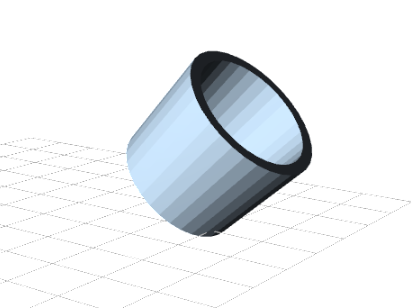
\includegraphics[keepaspectratio=true,width=0.75\textwidth]{expertmode/support/support_minimug_45deg.png}
\caption{Mod\`ele Minimug, inclin\'e \`a 45°.}
\label{fig:support_minimug_45deg}
\end{figure}

Comme avec le remplissage, il existe plusieurs motifs disponibles pour la structure de support.

\begin{figure}[H]
\centering
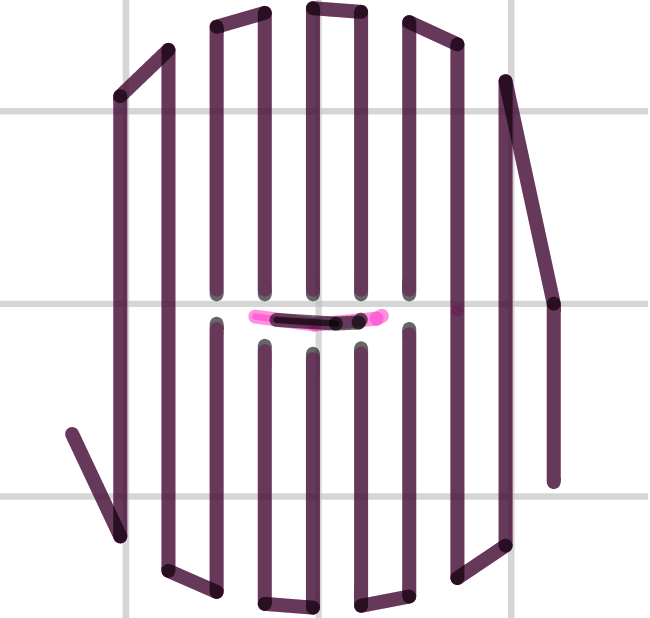
\includegraphics[keepaspectratio=true,width=0.2\textwidth]{expertmode/support/support_pattern_rectlinear.png}
\caption{Motif de support: Rectiligne}
\label{fig:support_pattern_rectlinear}
\end{figure}

\begin{figure}[H]
\centering
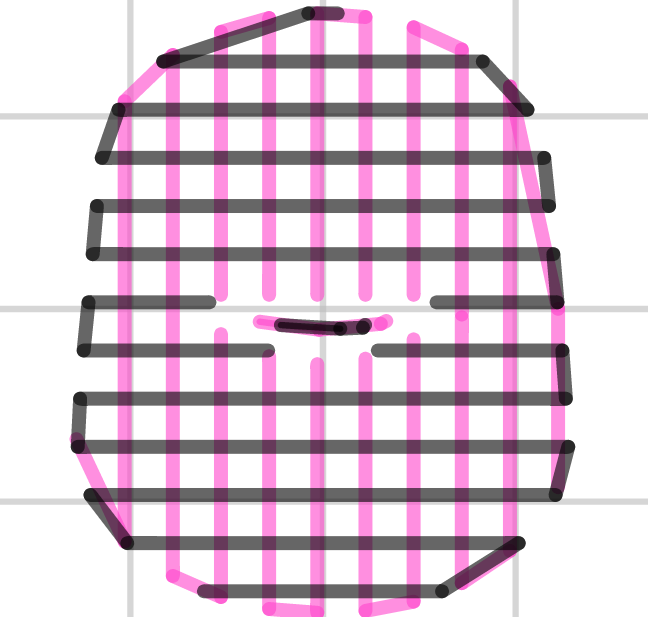
\includegraphics[keepaspectratio=true,width=0.2\textwidth]{expertmode/support/support_pattern_rectlinear_grid.png}
\caption{Motif de support: Grille Rectiligne}
\label{fig:support_pattern_rectlinear_grid}
\end{figure}

\begin{figure}[H]
\centering
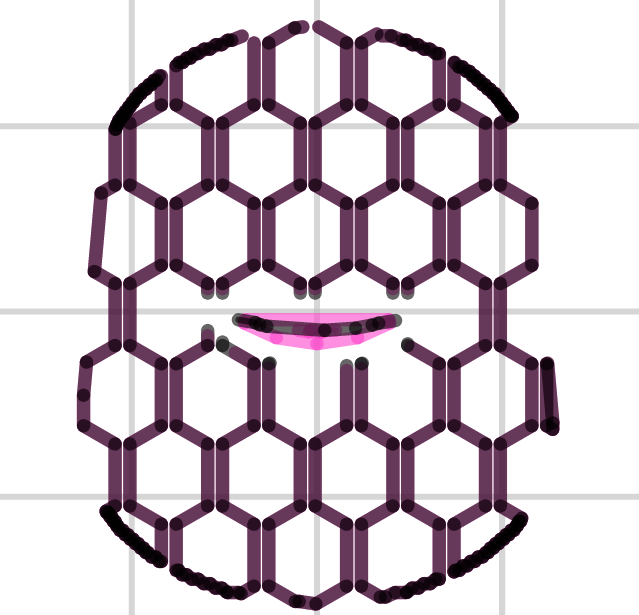
\includegraphics[keepaspectratio=true,width=0.2\textwidth]{expertmode/support/support_pattern_honeycomb.png}
\caption{Motif de support: Nid d'Abeille}
\label{fig:support_pattern_honeycomb}
\end{figure}
\index{Print Settings!Support material!Pattern Spacing}
\index{Param\`etres d'Impression!Mati\`ere de Support!Espacement du Motif}

\index{Print Settings!Support material!Pattern Angle}
\index{Param\`etres d'Impression!Mati\`ere de Support!Angle du Motif}

\texttt{Pattern Spacing} (Espacement du Motif) d\'etermine la distance entre les lignes de support, et est comparable \`a la densit\'e de remplissage en plus d'\^etre d\'efinie seulement en mm. Si vous changez cet attribut tenez compte de la largeur de l'extrusion du support et de la quantit\'e de mati\`ere de support qui adh\`ere \`a l'objet.

Il faut prendre soin de choisir un motif de support qui correspond au mod\`ele, o\`u le support se fixe perpendiculairement \`a la paroi de l'objet, plut\^ot que parall\`element, de sorte qu'il sera facile \`a retirer.  Si la structure de support court le long de la longueur d'une paroi alors le param\`etre \texttt{Pattern Angle} (Angle du Motif) permet la rotation de la direction des lignes de support

\begin{figure}[H]
\centering
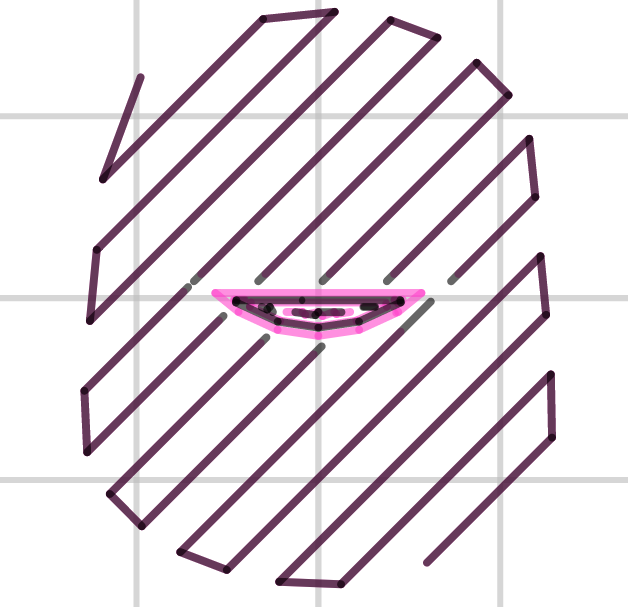
\includegraphics[keepaspectratio=true,width=0.2\textwidth]{expertmode/support/support_pattern_rectlinear_rotated.png}
\caption{Example de motif tourn\'e \`a 45°.}
\label{fig:support_pattern_rectlinear_rotated}
\end{figure}


%TODO: Interface layers.


% section support (end)

\newpage

%!TEX root = Slic3r-Manual.tex

\section{Extrudeuse Multiples} % (fold)
\label{sec:multiple_extruders}
\index{extruders!multiple}
\index{extrudeuse!multiple}

Une imprimante avec plus d'une extrudeuse peut \^etre utilis\'e de diff\'erentes mani\`eres: L'extrudeuse suppl\'ementaire pourrait imprimer une couleur ou une mati\`ere diff\'erente, ou pourrait \^etre attribu\'e \`a l'impression de caract\'eristiques particuli\`eres, telles que le remplissage, le support ou les p\'erim\`etres.

L'impression multi-mati\`eres n\'ecessite un objet conçu de mani\`ere appropri\'ee g\'en\'eralement \'ecrits au format AMF qui peut g\'erer plusieurs mat\'eriaux (voir les mod\`ele de format au §\ref{sub:model_formats}).  Les d\'etails sur la façon de cr\'eer de tel fichier sont donn\'es ci-dessous.


\subsection{Configurer les Extrudeuses} % (fold)
\label{sub:configuring_extruders}
\index{Printer Settings!General!Capabilities!Extruders}
\index{Param\`etres de l'Imprimante!Fonctionnalit\'es!Extrudeuses}

Dans l'onglet \texttt{Printer Settings} (Param\`etres de l'Imprimante) il y a le param\`etre \texttt{Extruders} (Extrudeuses), dans la section \texttt{Capabilities} (Fonctionnalit\'es), ce qui permet de d\'efinir le nombre d'extrudeuses. Incr\'ementer cette valeur ajouter dynamiquement une autre d\'efinition d'extrudeuse dans le volet de gauche.

\begin{figure}[H]
\centering
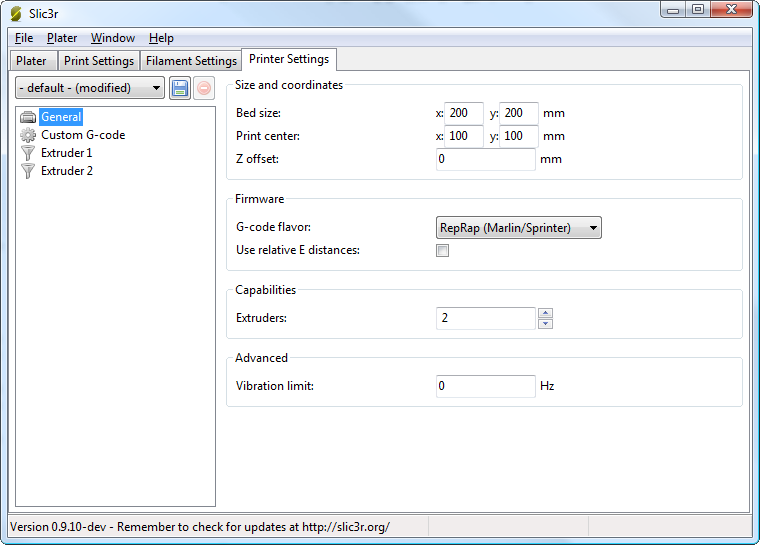
\includegraphics[keepaspectratio=true,width=1\textwidth]{expertmode/multipleextruders/printer_settings_general_multiple_extruder_options.png}
\caption{Param\`etres d'Extrudeuses Multiples - Onglet Param\`etre de l'Imprimante (G\'en\'eral).  Notez les deux extrudeuses d\'efinies dans le volet de gauche.}
\label{fig:printer_settings_general_multiple_extruder_options}
\end{figure}

Chaque extrudeuse peut \^etre configur\'e comme d'habitude, mais il ya d'autres param\`etres qui doivent \^etre d\'efinis qui sont notamment les configurations multi-extrudeuse.

\begin{figure}[H]
\centering
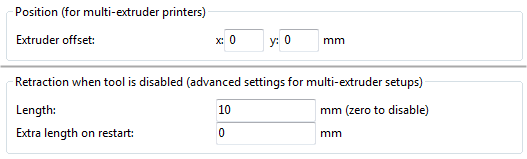
\includegraphics[keepaspectratio=true,width=1\textwidth]{expertmode/multipleextruders/printer_settings_extruder_multiple_extruder_options.png}
\caption{Param\`etres d'Extrudeuses Multiples - Onglet Param\`etre de l'Imprimante (Extruder).}
\label{fig:printer_settings_extruder_multiple_extruder_options}
\end{figure}

\index{Printer Settings!Extruder!Extruder offset}
\index{Param\`etres de l'Imprimante!D\'ecalage de l'extrudeuse}

l'\texttt{Extruder offset} (D\'ecalage de l'extrudeuse) doit \^etre utilis\'e si le microprogramme ne g\`ere pas le d\'ecalage de chaque buse suppl\'ementaire. La documentation de votre micrologiciel devrait vous dire si c'est le cas. Chaque extrudeuse suppl\'ementaire a un d\'ecalage par rapport \`a la premi\`ere. Si le firmware le g\`ere , toutes les compensations peuvent rester \`a 0,0.

\index{Printer Settings!Extruder!Retraction!Length}
\index{Param\`etres de l'Imprimante!Extrudeuse!R\'etractation!Longueur}
Parce que l'extrudeuse secondaire sera en sommeil tandis que la premi\`ere est cours d'utilisation, et vice-versa, il est important que le mat\'eriau soit suffisamment r\'etract\'ee pour cesser le suintement.  Comme avec les r\'eglages ordinaires de r\'etractation (voir p. \pageref{fig:retraction_settings}) le param\`etre \texttt{Length} (Longueur) est mesur\'ee \`a partir du filament entrant dans l'extrudeuse.

% subsection configuring_extruders (end)

\subsection{Attribution de filaments} % (fold)
\label{sub:assigning_filaments}
\index{Plater}
\index{Surface de Travail}
Quand un profil d'imprimante avec plusieurs extrudeuses a \'et\'e s\'electionn\'e, l'onglet \texttt{Plater} (Surface de Travail) permet la s\'election d'un filament diff\'erent pour chaque extrudeuse.

\begin{figure}[H]
\centering
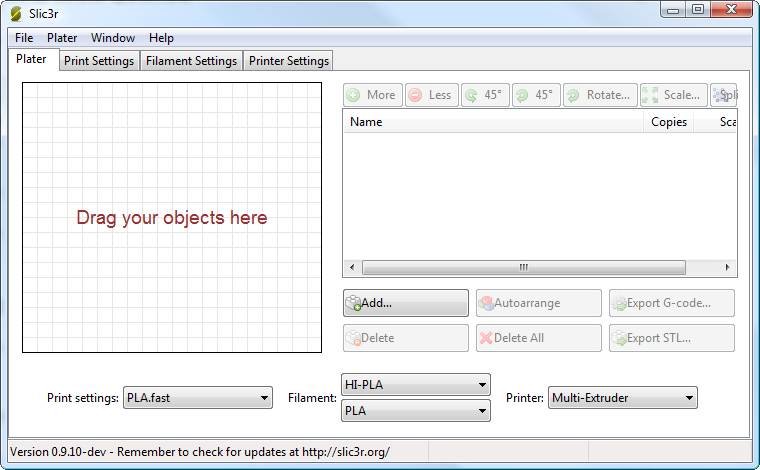
\includegraphics[keepaspectratio=true,width=1\textwidth]{expertmode/multipleextruders/plater_multi_filament.png}
\caption{Surface de travail avec de multiple param\`etre de filaments.}
\label{fig:plater_multi_filament}
\end{figure}

% subsection assigning_filaments (end)

\subsection{Affectation des extrudeuses pour les objets mono-mati\`ere} % (fold)
\label{sub:assigning_extruders}
\index{Print Settings!Multiple Extruders}
\index{Param\`etres de l'Imprimante!Extrudeuse Multiple}

Pour les impressions de mat\'eriaux unique, o\`u l'extrudeuse secondaire a pour mission une extrusion particuliere, la section \texttt{Multiple Extruders} (Extrudeuses multiples) de l'onglet \texttt{Print Settings} (Param\`etres de l'imprimante) donne la possibilit\'e d'assigner une extrudeuse pour chaque type d'extrusion.

\begin{figure}[H]
\centering
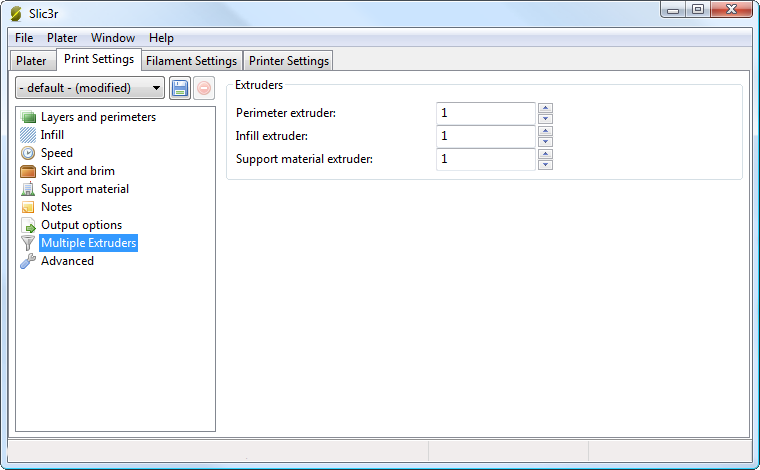
\includegraphics[keepaspectratio=true,width=1\textwidth]{expertmode/multipleextruders/print_settings_multiple_extruder_options.png}
\caption{Param\`etres d'Extrudeuse Multiple - Onglet Param\`etre d'Impression.}
\label{fig:advanced_multiple_extruder_options}
\end{figure}

% subsection assigning_extruders (end)

\subsection{Configurer le Changement d'Outil} % (fold)
\label{sub:configuring_tool_changes}

\index{Printer Settings!Custom G-code!Tool change G-code}
\index{Param\`etres de l'Imprimante!G-code personalis\'e!G-code de changement d'outil}

La section \texttt{Custom G-code} (G-code personalis\'e) de l'onglet \texttt{Printer Settings} (Param\`etres de l'Imprimante) dispose d'une option d'insertion de G-code entre les changements d'outils. Comme avec toutes les sections personnalis\'e G-code, les variables d'environement peuvent \^etre utilis\'ees afin de r\'ef\'erencer les param\`etres Slic3r.  Cela inclus les variables [previous\_extruder] et [next\_extruder].

\begin{figure}[H]
\centering
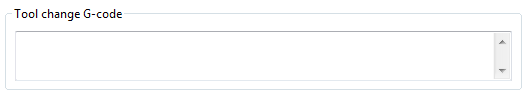
\includegraphics[keepaspectratio=true,width=1\textwidth]{expertmode/multipleextruders/printer_settings_custom_gcode.png}
\caption{Param\`etres d'Extrudeuse Multiple - G-code de Changement d'outil.}
\label{fig:printer_settings_custom_gcode}
\end{figure}

% subsection configuring_tool_changes (end)


\subsection{Impression d'objets multi-mati\`eres} % (fold)
\label{sub:printing_multi_material_objects}

Si un fichier multi-mat\'eriaux AMF existe d\'ej\`a, parce que le programme de CAO peut exporter un tel format, alors celui-ci peut \^etre charg\'e dans Slic3r de façon habituelle. Le mappage entre mati\`eres de l'objet et les extrudeuses est s\'equentielle, c'est \`a dire que la premiere mati\`ere est affect\'e \`a la premi\`ere extrudeuse, etc.

% subsection printing_multi_material_objects (end)


\subsection{G\'en\'eration de fichiers AMF multi-mati\`ere} % (fold)
\label{sub:generating_multi_material_amf_files}

Slic3r a la capacit\'e de combiner plusieurs fichiers STL dans un fichier multi-mati\`ere AMF.

\index{Menu!Combine multi-material STL files...}
\index{Menu!Combiner des fichiers STL multi-mati\`ere...}

\begin{itemize}
    \item Diviser la conception originale dans les diff\'erentes parties au sein du programme de CAO, et exporter chaque partie en STL.
    \item Dans Slic3r, choisissez \texttt{Combine multi-material STL files...} (Combiner des fichiers STL multi-mati\`ere...) a partir du menu \texttt{File} (Fichier).
    \item Lorsque vous \^etes invit\'e avec une bo\^ite de dialogueChoisissez le premier STL, qui sera attribu\'e \`a la premi\`ere mati\`ere (et donc la premi\`ere extrudeuse). Cliquez sur \texttt{Open} pour \^etre invit\'e au prochain STL, et ainsi de suite jusqu'\`a ce que chaque STL soit affect\'es \`a une mati\`ere. Pour signaler qu'il n'y a plus de fichiers STL, choisissez \texttt{Cancel} (Annuler).
    \item La bo\^ite de dialogue suivante demande l'emplacement et le nom du fichier de l'AMF.
\end{itemize}

Une fois g\'en\'er\'e le fichier peut \^etre charg\'e et imprim\'e comme d\'ecrit ci-dessus.

% subsection generating_multi_material_amf_files (end)

% section multipe_extruders (end)

\newpage

%!TEX root = Slic3r-Manual.tex

\section{Largeur d'Extrusion} % (fold)
\label{sec:extrusion_width}
\index{extrusion width}
\index{largeur d'extrusion}

\begin{figure}[H]
\centering
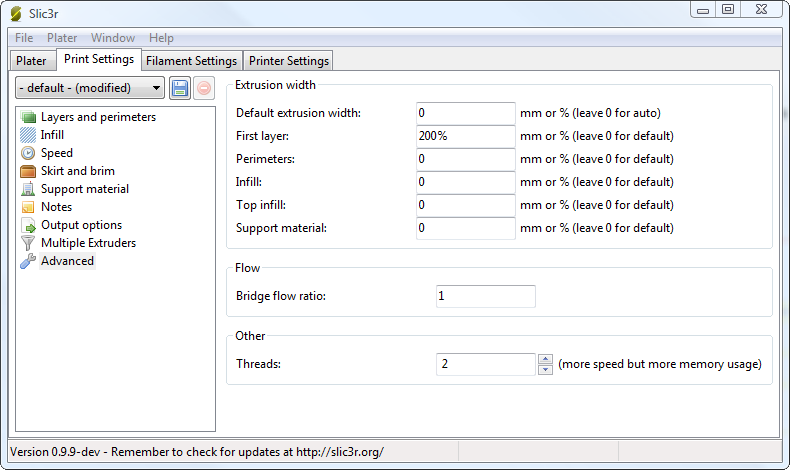
\includegraphics[keepaspectratio=true,width=1\textwidth]{expertmode/advanced_extrusion_widths_options.png}
\caption{Paramètres de largeur d'Extrusion.}
\label{fig:advanced_extrusion_widths_options}
\end{figure}

Une des raisons de la modification de la largeur de l'extrusion a déjà été examinée: l'augmentation de la largeur d'extrusion de la première couche dans le but d'améliorer l'adhesion au lit. (voir p.\pageref{par:wider_extrusion_width}).  Il ya quelques autres cas où il peut être bénéfique de modifier la largeur d'extrusion.
\begin{itemize}
    \item \texttt{Perimeter} (Périmètre) - Une valeur plus faible produira des extrusions minces qui à leurs tour produiront des surfaces plus précise.
    \item \texttt{Infill} (Remplissage) et \texttt{Solid Infill} (Remplissage solide) - Une extrusion épaisse pour le remplissage produira des impressions plus rapides et des pièces plus solides.
    \item \texttt{Top infill} (Remplissage suppérieur) - Une extrusion fine, améliorera la finition de la surface et assurera que es coins soit bien remplis.
    \item \texttt{Support material} (Matière de Support) - Comme avec les options de remplissage, une extrusion épaisse permettra de réduire le temps d'impression.
\end{itemize}

Il est important de se rappeler que, si la largeur de l'extrusion est exprimée en pourcentage, elle se calcule à partir de la propriété \texttt{Layer height} (Hauteur de couche), et non du paramètre \texttt{Default extrusion width} (Largeur d'extrusion par défaut).

% section extrusion_width (end)

\newpage

%!TEX root = Slic3r-Manual.tex

\section{Hauteur de couche variable} % (fold)
\label{sec:variable_layer_height}
\index{layer height}
\index{hauteur de couche}

Slic3r donne la possibilité de régler la hauteur de couche entre des positions arbitraires le long de l'axe Z. Voilà, des parties du modèle peuvent être imprimés avec une hauteur de couche grossière, par exemple des sections verticales, et d'autres parties pourraient être imprimés avec une hauteur de couche plus fine, par exemple les dégradés inclinés où les couches apparaissent plus marquées.

Le modèle de la fig. \ref{fig:example_model} donne un exemple rudimentaire où des hauteurs de couche variables pourraient être utilisées pour améliorer la qualité d'impression.  Les murs de la structure n'ont pas à être imprimés en haute définition pour une qualité acceptable, mais la pente du toit apparait en escalier, une hauteur de couche de 0,4 mm est trop grossière, en particulier pour la couche supérieure, qui est aplatie.  Ceci est illustré dans le G-Code représenté à la fig \ref{fig:example_gcode_normal_layer_heights}.


\begin{figure}[H]
\centering
\includegraphics[keepaspectratio=true,width=0.75\textwidth]{expertmode/variable_layer_height/example_model.png}
\caption{Exemple de modèle mettant en evidence un cas d'utilisation des couches variables.}
\label{fig:example_model}
\end{figure}

\begin{figure}[H]
\centering
\includegraphics[keepaspectratio=true,width=0.75\textwidth]{expertmode/variable_layer_height/example_gcode_normal_layer_heights.png}
\caption{Exemple avec des couches normales.}
\label{fig:example_gcode_normal_layer_heights}
\end{figure}

Les paramètres de hauteur de couche variables sont disponibles en double-cliquant sur ​​le nom de la pièce dans la fenêtre Plater (surface de travail).  Cela ouvrira une fenêtre qui contient deux onglets. Le premier donne des informations sur le modèle, comme indiqué dans la fig. \ref{fig:variable_layer_height_options_tab_1}.

\begin{figure}[H]
\centering
\includegraphics[keepaspectratio=true,width=0.75\textwidth]{expertmode/variable_layer_height/variable_layer_height_options_tab_1.png}
\caption{Paramètres de Couche variable - Info.}
\label{fig:variable_layer_height_options_tab_1}
\end{figure}

Il convient de noter la hauteur du modèle, puisque cela sera utile pour le calcul de la hauteur maximale de Z.

Le deuxième onglet (fig. \ref{fig:variable_layer_height_options_tab_2}) présente un tableau dans lequel chaque rangée définit une hauteur de couche pour une plage particulière le long de l'axe Z, exprimée en millimètres. Dans cet exemple, les parois du modèle sont imprimés à 0,4 mm, les parties raides du toit sont imprimées à 0,2 mm, et la moins raide à 0,15 mm. Notez que chaque plage se divise exactement par la hauteur de la couche donnée de sorte qu'il n'y a pas de «trous» entre les sections.

\begin{figure}[H]
\centering
\includegraphics[keepaspectratio=true,width=0.75\textwidth]{expertmode/variable_layer_height/variable_layer_height_options_tab_2.png}
\caption{Paramètres de Couche variable - Layers (Couches).}
\label{fig:variable_layer_height_options_tab_2}
\end{figure}

Le G-Code résultant (fig. \ref{fig:example_gcode_variable_layer_heights}) montre une plus haute définition qui devrait aboutir à une impression de qualité supérieure.

\begin{figure}[H]
\centering
\includegraphics[keepaspectratio=true,width=0.75\textwidth]{expertmode/variable_layer_height/example_gcode_variable_layer_heights.png}
\caption{Example avec une hauteur de couche variable.}
\label{fig:example_gcode_variable_layer_heights}
\end{figure}

La Fig. \ref{fig:example_print} montre le modèle d'exemple imprimé.  L'impression de la gauche a 0,4 mm hauteur de la couche partout, alors que l'impression sur la droite a la hauteur de la couche variable.

\begin{figure}[H]
\centering
\includegraphics[keepaspectratio=true,width=1\textwidth]{expertmode/variable_layer_height/example_print.jpg}
\caption{Exemple d'impression avec une hauteur de couches variable.}
\label{fig:example_print}
\end{figure}

Une caractéristique supplémentaire de l'option de hauteur de couches variable est que par la saisie d'un zéro pour une plage de la partie du modèle ne sera pas imprimé.  Fig. \ref{fig:example_gcode_skipped_layers} shows the G-Code where layers between 0 and 4mm are skipped.  This is a useful way of dividing a tall model into multiple, shorter sections which can be printed individually and assembled afterwards.
\begin{figure}[H]
\centering
\includegraphics[keepaspectratio=true,width=0.75\textwidth]{expertmode/variable_layer_height/example_gcode_skipped_layers.png}
\caption{Exemple avec des couches ignorés.}
\label{fig:example_gcode_skipped_layers}
\end{figure}

% section variable_layer_height (end)
}
\fi
%%% END EXPERT MODE %%%

%%% CONFIGURATION ORGANIZATION %%%
\ifadvanced
\chapter{\emph{Organisation de la Configuration}}
\thispagestyle{empty}
\markboth{Organisation de la Configuration}{Manuel Utilisateur de Slic3r}
{%!TEX root = Slic3r-Manual.tex

Il ya deux façons d'organiser les paramètres de configuration: exporter et importer les paramètres de configuration, et des profils. Le premier est disponible en mode simple et expert, alors que les profils sont disponibles uniquement en mode expert.

\section{Export et Import de la Configuration} % (fold)
\label{sub:exporting_and_importing_configuration}
\index{configuration!export}
\index{configuration!import}

L'ensemble actuel d'options de configuration peut être tout simplement exporté via le menu File (Fichier)  \texttt{Export Config}. Cela permet se sauvegarder toutes les valeurs dans un fichier texte avec l'extention \texttt{.ini} .  Les fichiers précédemment enregistrés peuvent être chargés avec le menu File (Fichier) \texttt{Load Config} (charger la configuration).

Cela donne un des moyens rudimentaires pour stocker des paramètres de configuration pour les différents besoins. Par exemple, un ensemble avec des vitesses d'impression légèrement plus rapides, ou un motif de remplissage différent. Cependant, cette façon d'organiser les choses va vite devenir frustrante, car chaque changement mineur d'un paramètre pourrait être à dupliqué dans de nombreuses configurations. Pour cette raison, les profils sont de façon plus appropriée de gérer plusieurs configurations.

Cette méthode permet également le transfert de configurations entre machines, ou le stockage à distance.

% section exporting_and_importing_configuration (end)


\section{Profils} % (fold)
\label{sec:profiles}
\index{profiles}
\index{profils}

Après quelques impressions, il deviendra évident qu'il est utile d'avoir un ensemble d'options de configuration à choisir, et que certains paramètres changent plus souvent que d'autres. En mode expert, des profils peuvent être créés pour les paramètres d'impression, de Filament et d'imprimante, dans l'espoir que les paramètres d'imprimante changent peu souvent, de filaments rarement, cependant les paramètres d'impression peuvent être modifiés pour chaque modèle. Ces différents profils peuvent être mélangés et combinés à volonté, et peuvent être sélectionnés dans leurs onglets respectifs, ou directement à partir de la surface de travail.

\subsection{Création des Profils} % (fold)
\label{sub:creating_profiles}
\index{profiles!create}
\index{profils!création}

Ouvrez l'onglet souhaité et modifiez les paramètres si nécessaire. Une fois satisfait, cliquez sur l'icône de sauvegarde vers la gauche au-dessus des titres de réglage, et donner un nom approprié à l'invite.

\begin{figure}[H]
\centering
\includegraphics[keepaspectratio=true,width=1\textwidth]{organising/creating_a_profile.png}
\caption{Sauver un profil.}
\label{fig:creating_a_profile}
\end{figure}

\index{profiles!delete}
\index{profils!effacer}
Les profils peuvent être supprimés, en choisissant le profil à supprimer et en cliquant sur le bouton rouge supprimer à côté du bouton Enregistrer.

\begin{figure}[H]
\centering
\includegraphics[keepaspectratio=true,width=1\textwidth]{organising/deleting_a_profile.png}
\caption{Effacer un profil.}
\label{fig:deleting_a_profile}
\end{figure}

% subsection creating_profiles (end)


% section profiles (end)}
\fi
%%% END CONFIGURATION ORGANIZATION %%%

%%% REPAIRING MODELS %%%
\ifadvanced
\chapter{\emph{R\'eparer Les mod\`eles}}
\thispagestyle{empty}
\markboth{R\'eparer Les mod\`eles}{Manuel Utilisateur de Slic3r}
{%!TEX root = Slic3r-Manual.tex

Si le maillage 3D d\'ecrit dans le mod\`ele contient des trous, ou les bords ne sont pas align\'es (connu comme \'etant non-manifold), alors Slic3r peut avoir des probl\`emes de traitement . Slic3r va tenter de r\'esoudre les probl\`emes, s'il le peut, mais certains probl\`emes sont hors de sa port\'ee. Si l'application indique que le mod\`ele ne peut pas \^etre tranch\'e correctement alors il ya plusieurs options disponibles, et celles d\'ecrites ici sont tous libres au moment de l'\'ecriture.

%%% CONFIGURATION TUNING %%%
{%!TEX root = Slic3r-Manual.tex

\paragraph{Netfabb Studio} % (fold)
\label{par:netfabb_studio}
Netfabb produit une gamme d'applications de modélisation 3D, y compris une version de base gratuite\footnote{http://www.netfabb.com/basic.php}.  Cette version comprend un module de réparation de maillage qui peut aider à éliminer les différents problèmes rencontrés. Les instructions mise à jour peuvent être trouvés sur le wiki Netfabb\footnote{http://wiki.netfabb.com/Part\_Repair}, ce qui suit est un bref aperçu des étapes à suivre.

\begin{figure}[H]
\centering
\includegraphics[keepaspectratio=true,width=0.75\textwidth]{working_with_models/netfabb_studio_part_repair.png}
\caption{Netfabb Studio: Réparation de modèle.}
\label{fig:netfabb_studio_part_repair}
\end{figure}

\begin{itemize}
	\item Lancer Netfabb studio, et charger le fichier STL qui a un problème, que ce soit par l'intermédiaire du menu \texttt{File} ou par glisser-déposer sur l'espace de travail. Si Netfabb détecte un problème, il affiche un signe d'alerte rouge dans le coin en bas à droite.
	\item Pour exécuter les scripts de réparation, sélectionnez la partie et puis cliquez sur la première icône d'aide dans la barre d'outils (la croix rouge), ou sélectionnez dans le menu contextuel \texttt{Extras->Repair Part}.  Cela va ouvrir l'onglet réparation de modèle et de montrer l'état du modèle.
	\item Les onglets \texttt{Actions} et \texttt{Repair scripts} offrent plusieurs scripts de réparation qui peuvent être appliquées manuellement, mais dans le but de cet aperçu sélectionez le script \texttt{Automatic repair} corrigera la plupart des problèmes.
	\item Le bouton de réparation automatique présente deux options: par défaut et simples. Choisir par défaut couvrira la plupart des cas. Selectionnez \texttt{execute} pour lancer le script.
	\item Une fois la pièce réparée les réparations doivent être appliquées en sélectionnant \texttt{Apply repair}, choisissant s'il faut passer outre la partie existante ou non.
	\item La pièce peut ensuite être exporté en sélectionnant \texttt{Export part->As STL} à partir du menu contextuel.
	\item Si Netfabb détecte encore que la partie exportée contient des erreurs, alors il offrira la possibilité d'appliquer d'autres réparations avant de l'exporter.
	\begin{figure}[H]
	\centering
	\includegraphics[keepaspectratio=true,width=0.75\textwidth]{working_with_models/netfabb_studio_export_part.png}
	\caption{Netfabb Studio: Export de pièce.}
	\label{fig:netfabb_studio_export_part}
	\end{figure}
\end{itemize}
% paragraph netfabb_studio (end)

\paragraph{Netfabb Cloud Service} % (fold)
\label{par:netfabb_cloud_service}
Netfabb accueille également un service web où un fichier STL peut être téléchargé pour être vérifié et réparé\footnote{http://cloud.netfabb.com/}.  

\begin{figure}[H]
\centering
\includegraphics[keepaspectratio=true,width=0.75\textwidth]{working_with_models/netfabb_cloud_services.png}
\caption{Netfabb Cloud Services.}
\label{fig:netfabb_cloud_services}
\end{figure}

\begin{itemize}
	\item Accédez à http://cloud.netfabb.com
	\item Choisissez le fichier STL à télécharger en utilisant le bouton prévu.
	\item Une adresse e-mail doit être donnée pour vous informer quand la prestation est terminé.
	\item Choisissez entre les mesures métriques ou impériales qui doivent être utilisés.
	\item Lisez et acceptez les conditions de service, puis cliquez sur \texttt{Upload to Cloud}.
	\item Une fois que le service a analysé et réparé le fichier, un email est envoyé, fournissant le lien de téléchargement du fichier réparé.
\end{itemize}
}
%%% END CONFIGURATION TUNING %%%

\paragraph{FreeCAD} % (fold)
\label{par:freecad}
\index{FreeCAD}

Freecad\footnote{\url{http://sourceforge.net/projects/free-cad}} est un logiciel de CAO, complet et gratuit, qui est livr\'e avec un module de maillage, dans lequel on peut effectuer les r\'eparations d'erreur dans les mod\`eles. Les \'etapes suivantes d\'ecrivent comment un probl\`eme dans un fichier de mod\`ele peut \^etre analys\'e et r\'epar\'e.

\begin{figure}[H]
\centering
\includegraphics[keepaspectratio=true,width=0.75\textwidth]{working_with_models/freecad_part_repair.png}
\caption{R\'eparation avec FreeCAD.}
\label{fig:freecad_part_repair}
\end{figure}

\begin{itemize}
	\item Lancer FreeCAD et \`a partir la page d'accueil choisir \texttt{Working with Meshes}.
	\item Chargez le mod\`ele en le faisant glisser sur l'espace de travail ou par l'interm\'ediaire du menu \texttt{File}.  Un petit message dans le coin en bas \`a gauche indique si le mod\`ele semble avoir des probl\`emes.
	\item Dans le menu choisissez \texttt{Meshes->Analyze->Evaluate \& Repair mesh} pour faire appara\^itre la bo\^ite de dialogue des options de r\'eparation.
	\item Dans la bo\^ite de dialogue choisir la maille charg\'ee, puis effectuer chaque analyse soit en cliquant sur le bouton \texttt{Analyze} par type de probl\`eme, ou s\'electionnez \texttt{Repetitive Repair} en bas pour effectuer tous les contr\^oles. Si un probl\`eme  correspondant est d\'etect\'e le bouton \texttt{Repair} devient actif.
	\item Pour chaque r\'eparation souhait\'e frapp\'e le bouton \texttt{Repair}.
	\item Il est important d'examiner l'effet que le script de r\'eparation a apport\'ees au mod\`ele.  Il se peut que le script produise des dommages dans le fichier, plut\^ot que de le r\'eparer, par exemple en retirant triangles importants.
	\item Exporter le mod\`ele r\'epar\'e par le menu \texttt{Export} ou le menu contextuel.
\end{itemize}
% paragraph freecad (end)
}
\fi
%%% END REPAIRING MODELS %%%

%%% ADVANCED %%%
\ifadvanced
\chapter{\emph{Sujets Avanc\'es}}
\thispagestyle{empty}
\markboth{Sujets Avanc\'es}{Manuel Utilisateur de Slic3r}
{%!TEX root = Slic3r-Manual.tex

%!TEX root = Slic3r-Manual.tex

\section{Impression S\'equentielle} % (fold)
\label{sec:sequential_printing}
\index{Sequential Printing}
\index{Impression S\'equentielle}

Lors de l'impression de plusieurs objets \`a la fois, il peut \^etre utile d'imprimer chacun s\'epar\'ement, ce qui r\'eduira le suintement et les ficelles se formant entre les impressions. Cela permettra aussi de r\'eduire le risque qu''un probl\`eme ne ruine toute l'impression - si une partie se d\'etache ou \'echoue d'une certaine mani\`ere, il ne sera pas tra\^in\'e dans d'autres parties de l'impression \`a chaque couche.

\begin{figure}[H]
\centering
\includegraphics[keepaspectratio=true,width=1\textwidth]{simple_mode/sequential_printing_options.png}
\caption{Options d'impression s\'equentielle.}
\label{fig:sequential_printing_options}
\end{figure}

\index{Print Settings!Output options!Sequential printing!Extruder clearance}
\index{Param\`etres d'Impression!Options de sortie!Impression s\'equentielle!D\'egagement de l'extrudeuse}
Un soin doit \^etre pris afin que la buse et extrudeuse n'interf\`ere pas avec les parties d\'ej\`a imprim\'ees.  Slic3r devrait avertir s'il d\'etecte que la buse ou l'extrudeuse peuvent entrer en collision avec une pi\`ece, mais v\'erifiez que la disposition des pi\`eces ne puisse pas causer de probl\`eme.  Le param\`etre \texttt{Extruder clearance} (D\'egagement de l'extrudeuse) aide Slic3r \`a d\'etecter les risques de collision:
\begin{itemize}
	\item \texttt{Radius} (Rayon) - Le d\'egagement qui devrait \^etre accord\'ee autour de l'extrudeuse. Prenez soin si l'extrudeuse n'est pas mont\'e au centre - prendre la plus grande valeur par s\'ecurit\'e.
	\item \texttt{Height} (Hauteur) - La distance verticale entre la buse et les tiges de l'axe X, ou partie la plus basse qui peut interf\'erer avec une impression finale.
\end{itemize}

\begin{figure}[H]
\centering
\includegraphics[keepaspectratio=true,width=0.5\textwidth]{simple_mode/extruder_clearance.jpg}
\caption{Le cylindre de d\'egagement autour de l'extrudeuse.}
\label{fig:a_diagram_depicting_extruder_clearance}
\end{figure}



\newpage

%!TEX root = Slic3r-Manual.tex

\section{Sortie SVG} % (fold)
\label{sec:svg_output}
\index{SVG}
\index{DLP resin printer}
\index{imprimante r\'esine DLP}
\index{powder-bed printer}
\index{imprimante \`a poudre}

Slic3r peut produire une sortie pour d'autres types d'imprimantes 3D qui n\'ecessitent que chaque couche soit repr\'esent\'e en image, par exemple les imprimante r\'esine DLP ou \`a poudre-lit. Ces imprimantes attendent une image g\'en\'eralement constitu\'e d'une silhouette blanche sur un fond noir (voir figure \ref{fig:example_svg_slice}).  Presque tous les formats d'image peuvent \^etre utilis\'es (bmp, png, etc), cependant, parce que l'image peut \^etre r\'eduite, il est g\'en\'eralement souhaitable d'utiliser un format vectoriel, plut\^ot qu'un format bitmap. Pour cette raison, il est courant d'utiliser le format "Scalable Vector Graphics" (SVG).

\begin{figure}[H]
\centering
\includegraphics[keepaspectratio=true,width=0.5\textwidth]{advanced/svg_output/example_svg_slice.png}
\caption{Example de tranche SVG.}
\label{fig:example_svg_slice}
\end{figure}

\index{Menu!Slice to SVG...}
\index{Menu!Trancher au format SVG...}

Slic3r offre la possibilit\'e de produire une sortie SVG appropri\'e pour de telles imprimantes.  Au lieu d'utiliser le \texttt{Plater}, le processus commence par la s\'election de l'option \texttt{Slice to SVG...} du menu \texttt{File}.  Celui-ci demande le fichier source (STL, OBJ ou AMF), et lorsqu'il est s\'electionn\'e demande o\`u le fichier SVG de sortie doit \^etre enregistr\'e. Ensuite Slic3r d\'emarre et produit le fichier SVG.

Tenter de voir le fichier SVG dans un navigateur entra\^inera seulement l'affichage de la premi\`ere couche, et seules les \^iles n\'egatifs dans le mod\`ele (comme l'arri\`ere-plan du navigateur est g\'en\'eralement blanc).

\begin{figure}[H]
\centering
\includegraphics[keepaspectratio=true,width=0.75\textwidth]{advanced/svg_output/svg_direct_browser.png}
\caption{le fichier SVG vu dans un navigateur.}
\label{fig:svg_direct_browser}
\end{figure}

Pour cette raison, une petite application web a \'et\'e \'ecrite pour permettre de visualiser chaque tranche sur un fond noir\footnote{\url{http://garyhodgson.github.io/slic3rsvgviewer}}.  Acc\'edez \`a l'application et faites glisser le fichier SVG sur l'\'ecran pour le charger et l'afficher.

\begin{figure}[H]
\centering
\includegraphics[keepaspectratio=true,width=0.75\textwidth]{advanced/svg_output/svg_slic3rsvg_viewer.png}
\caption{Slic3r SVG Viewer.}
\label{fig:svg_slic3rsvg_viewer}
\end{figure}

\subsection{Param\`etres SVG} % (fold)
\label{sub:svg_settings}

La majorit\'e des options dans Slic3r ne sont pas n\'ecessaires pour la g\'en\'eration SVG, cependant le param\`etre \texttt{Layer height} d\'eterminera le nombre de couches. Notez que Slic3r limite la hauteur de la couche pour qu'elle soit plus petite que le diam\`etre de la buse, donc cela peut \'egalement \^etre augmenter si l'on souhaite des couches plus hautes.

% subsection svg_settings (end)

\subsection{Imprimer \`a partir de fichiers SVG} % (fold)
\label{sub:printing_with_svg}

Alors que la sortie SVG peut \^etre utilis\'e pour une gamme d'imprimantes, l'exemple suivant montre comment le fichier, peut \^etre utilis\'e avec une imprimante r\'esine DLP. En utilisant une version modifi\'ee de Printrun \footnote{\url{http://garyhodgson.com/reprap/projectlayer}} le fichier SVG peut \^etre charg\'e directement et envoy\'e \`a un projecteur DLP. L'axe Z est contr\^ol\'ee par des commandes G-code envoy\'e par le composant printcore, ce qui signifie que l'\'electronique RepRap standard, tels que RAMPS, peuvent \^etre utilis\'es.


\begin{figure}[H]
\centering
\includegraphics[keepaspectratio=true,width=0.75\textwidth]{advanced/svg_output/projectlayer.png}
\caption{Impression SVG avec Projectlayer.}
\label{fig:projectlayer}
\end{figure}


% subsection printing_with_svg (end)

% section svg_output (end)

\newpage

%!TEX root = Slic3r-Manual.tex

\section{Command Line Usage} % (fold)
\label{sec:command_line_usage}
\index{command line}
\index{scripting}

Slic3r can also be used from the command line instead of via the GUI, as part of a script, or as part of another tool, such as Printrun\footnote{https://github.com/kliment/Printrun}.

All options found in the GUI can be used from the command line in the form of switch parameters.  The latest version of these are given below, and the most up-to-date information can be found by issuing the command: \par\texttt{slic3r.pl --help}

Preset configurations can be loaded from a .ini file using the \texttt{--load} option, and options can be overridden further on the command line, e.g. \par\texttt{slic3r.pl --load config.ini --layer-height 0.25 file.stl}

\subsection{Command Line Options} % (fold)
\label{sub:command_line_options}

\tiny
\begin{verbatim}

Usage: slic3r.pl [ OPTIONS ] file.stl

    --help              Output this usage screen and exit
    --version           Output the version of Slic3r and exit
    --save <file>       Save configuration to the specified file
    --load <file>       Load configuration from the specified file. It can be used
                        more than once to load options from multiple files.
    -o, --output <file> File to output gcode to (by default, the file will be saved
                        into the same directory as the input file using the
                        --output-filename-format to generate the filename)
    -j, --threads <num> Number of threads to use (1+, default: 2)

  GUI options:
    --no-plater         Disable the plater tab
    --gui-mode          Overrides the configured mode (simple/expert)

  Output options:
    --output-filename-format
                        Output file name format; all config options enclosed in brackets
                        will be replaced by their values, as well as [input_filename_base]
                        and [input_filename] (default: [input_filename_base].gcode)
    --post-process      Generated G-code will be processed with the supplied script;
                        call this more than once to process through multiple scripts.
    --export-svg        Export a SVG file containing slices instead of G-code.
    -m, --merge         If multiple files are supplied, they will be composed into a single
                        print rather than processed individually.

  Printer options:
    --nozzle-diameter   Diameter of nozzle in mm (default: 0.5)
    --print-center      Coordinates in mm of the point to center the print around
                        (default: 100,100)
    --z-offset          Additional height in mm to add to vertical coordinates
                        (+/-, default: 0)
    --gcode-flavor      The type of G-code to generate 
                        (reprap/teacup/makerbot/sailfish/mach3/no-extrusion, default: reprap)
    --use-relative-e-distances Enable this to get relative E values
    --gcode-arcs        Use G2/G3 commands for native arcs (experimental, not supported
                        by all firmwares)
    --g0                Use G0 commands for retraction (experimental, not supported by all
                        firmwares)
    --gcode-comments    Make G-code verbose by adding comments (default: no)
    --vibration-limit   Limit the frequency of moves on X and Y axes (Hz, set zero to disable;
                        default: 0)

  Filament options:
    --filament-diameter Diameter in mm of your raw filament (default: 3)
    --extrusion-multiplier
                        Change this to alter the amount of plastic extruded. There should be
                        very little need to change this value, which is only useful to
                        compensate for filament packing (default: 1)
    --temperature       Extrusion temperature in degree Celsius, set 0 to disable (default: 200)
    --first-layer-temperature Extrusion temperature for the first layer, in degree Celsius,
                        set 0 to disable (default: same as --temperature)
    --bed-temperature   Heated bed temperature in degree Celsius, set 0 to disable (default: 0)
    --first-layer-bed-temperature Heated bed temperature for the first layer, in degree Celsius,
                        set 0 to disable (default: same as --bed-temperature)

  Speed options:
    --travel-speed      Speed of non-print moves in mm/s (default: 130)
    --perimeter-speed   Speed of print moves for perimeters in mm/s (default: 30)
    --small-perimeter-speed
                        Speed of print moves for small perimeters in mm/s or % over perimeter speed
                        (default: 30)
    --external-perimeter-speed
                        Speed of print moves for the external perimeter in mm/s or % over perimeter speed
                        (default: 70%)
    --infill-speed      Speed of print moves in mm/s (default: 60)
    --solid-infill-speed Speed of print moves for solid surfaces in mm/s or % over infill speed
                        (default: 60)
    --top-solid-infill-speed Speed of print moves for top surfaces in mm/s or % over solid infill speed
                        (default: 50)
    --support-material-speed
                        Speed of support material print moves in mm/s (default: 60)
    --bridge-speed      Speed of bridge print moves in mm/s (default: 60)
    --gap-fill-speed    Speed of gap fill print moves in mm/s (default: 20)
    --first-layer-speed Speed of print moves for bottom layer, expressed either as an absolute
                        value or as a percentage over normal speeds (default: 30%)

  Acceleration options:
    --perimeter-acceleration
                        Overrides firmware's default acceleration for perimeters. (mm/s^2, set zero
                        to disable; default: 0)
    --infill-acceleration
                        Overrides firmware's default acceleration for infill. (mm/s^2, set zero
                        to disable; default: 0)
    --bridge-acceleration
                        Overrides firmware's default acceleration for bridges. (mm/s^2, set zero
                        to disable; default: 0)
    --default-acceleration
                        Acceleration will be reset to this value after the specific settings above
                        have been applied. (mm/s^2, set zero to disable; default: 130)

  Accuracy options:
    --layer-height      Layer height in mm (default: 0.4)
    --first-layer-height Layer height for first layer (mm or %, default: 0.35)
    --infill-every-layers
                        Infill every N layers (default: 1)
    --solid-infill-every-layers
                        Force a solid layer every N layers (default: 0)

  Print options:
    --perimeters        Number of perimeters/horizontal skins (range: 0+, default: 3)
    --top-solid-layers  Number of solid layers to do for top surfaces (range: 0+, default: 3)
    --bottom-solid-layers  Number of solid layers to do for bottom surfaces (range: 0+, default: 3)
    --solid-layers      Shortcut for setting the two options above at once
    --fill-density      Infill density (range: 0-1, default: 0.4)
    --fill-angle        Infill angle in degrees (range: 0-90, default: 45)
    --fill-pattern      Pattern to use to fill non-solid layers (default: honeycomb)
    --solid-fill-pattern Pattern to use to fill solid layers (default: rectilinear)
    --start-gcode       Load initial G-code from the supplied file. This will overwrite
                        the default command (home all axes [G28]).
    --end-gcode         Load final G-code from the supplied file. This will overwrite
                        the default commands (turn off temperature [M104 S0],
                        home X axis [G28 X], disable motors [M84]).
    --layer-gcode       Load layer-change G-code from the supplied file (default: nothing).
    --toolchange-gcode  Load tool-change G-code from the supplied file (default: nothing).
    --extra-perimeters  Add more perimeters when needed (default: yes)
    --randomize-start   Randomize starting point across layers (default: yes)
    --avoid-crossing-perimeters Optimize travel moves so that no perimeters are crossed (default: no)
    --external-perimeters-first Reverse perimeter order. (default: no)
    --only-retract-when-crossing-perimeters
                        Disable retraction when travelling between infill paths inside the same island.
                        (default: no)
    --solid-infill-below-area
                        Force solid infill when a region has a smaller area than this threshold
                        (mm^2, default: 70)
    --infill-only-where-needed
                        Only infill under ceilings (default: no)
    --infill-first      Make infill before perimeters (default: no)

   Support material options:
    --support-material  Generate support material for overhangs
    --support-material-threshold
                        Overhang threshold angle (range: 0-90, set 0 for automatic detection,
                        default: 0)
    --support-material-pattern
                        Pattern to use for support material (default: rectilinear)
    --support-material-spacing
                        Spacing between pattern lines (mm, default: 2.5)
    --support-material-angle
                        Support material angle in degrees (range: 0-90, default: 0)
    --support-material-interface-layers
                        Number of perpendicular layers between support material and object 
                        (0+, default: 0)
    --support-material-interface-spacing
                        Spacing between interface pattern lines 
                        (mm, set 0 to get a solid layer, default: 0)
    --raft-layers       Number of layers to raise the printed objects by (range: 0+, default: 0)
    --support-material-enforce-layers
                        Enforce support material on the specified number of layers from bottom,
                        regardless of --support-material and threshold (0+, default: 0)

   Retraction options:
    --retract-length    Length of retraction in mm when pausing extrusion (default: 1)
    --retract-speed     Speed for retraction in mm/s (default: 30)
    --retract-restart-extra
                        Additional amount of filament in mm to push after
                        compensating retraction (default: 0)
    --retract-before-travel
                        Only retract before travel moves of this length in mm (default: 2)
    --retract-lift      Lift Z by the given distance in mm when retracting (default: 0)
    --retract-layer-change
                        Enforce a retraction before each Z move (default: yes)
    --wipe              Wipe the nozzle while doing a retraction (default: no)

   Retraction options for multi-extruder setups:
    --retract-length-toolchange
                        Length of retraction in mm when disabling tool (default: 1)
    --retract-restart-extra-toolchnage
                        Additional amount of filament in mm to push after
                        switching tool (default: 0)

   Cooling options:
    --cooling           Enable fan and cooling control
    --min-fan-speed     Minimum fan speed (default: 35%)
    --max-fan-speed     Maximum fan speed (default: 100%)
    --bridge-fan-speed  Fan speed to use when bridging (default: 100%)
    --fan-below-layer-time Enable fan if layer print time is below this approximate number
                        of seconds (default: 60)
    --slowdown-below-layer-time Slow down if layer print time is below this approximate number
                        of seconds (default: 30)
    --min-print-speed   Minimum print speed (mm/s, default: 10)
    --disable-fan-first-layers Disable fan for the first N layers (default: 1)
    --fan-always-on     Keep fan always on at min fan speed, even for layers that don't need
                        cooling

   Skirt options:
    --skirts            Number of skirts to draw (0+, default: 1)
    --skirt-distance    Distance in mm between innermost skirt and object
                        (default: 6)
    --skirt-height      Height of skirts to draw (expressed in layers, 0+, default: 1)
    --min-skirt-length  Generate no less than the number of loops required to consume this length
                        of filament on the first layer, for each extruder (mm, 0+, default: 0)
    --brim-width        Width of the brim that will get added to each object to help adhesion
                        (mm, default: 0)

   Transform options:
    --scale             Factor for scaling input object (default: 1)
    --rotate            Rotation angle in degrees (0-360, default: 0)
    --duplicate         Number of items with auto-arrange (1+, default: 1)
    --bed-size          Bed size, only used for auto-arrange (mm, default: 200,200)
    --duplicate-grid    Number of items with grid arrangement (default: 1,1)
    --duplicate-distance Distance in mm between copies (default: 6)

   Sequential printing options:
    --complete-objects  When printing multiple objects and/or copies, complete each one before
                        starting the next one; watch out for extruder collisions (default: no)
    --extruder-clearance-radius Radius in mm above which extruder won't collide with anything
                        (default: 20)
    --extruder-clearance-height Maximum vertical extruder depth; i.e. vertical distance from
                        extruder tip and carriage bottom (default: 20)

   Miscellaneous options:
    --notes             Notes to be added as comments to the output file
    --resolution        Minimum detail resolution (mm, set zero for full resolution, default: 0)

   Flow options (advanced):
    --extrusion-width   Set extrusion width manually; it accepts either an absolute value in mm
                        (like 0.65) or a percentage over layer height (like 200%)
    --first-layer-extrusion-width
                        Set a different extrusion width for first layer
    --perimeter-extrusion-width
                        Set a different extrusion width for perimeters
    --infill-extrusion-width
                        Set a different extrusion width for infill
    --solid-infill-extrusion-width
                        Set a different extrusion width for solid infill
    --top-infill-extrusion-width
                        Set a different extrusion width for top infill
    --support-material-extrusion-width
                        Set a different extrusion width for support material
    --bridge-flow-ratio Multiplier for extrusion when bridging (> 0, default: 1)

   Multiple extruder options:
    --extruder-offset   Offset of each extruder, if firmware doesn't handle the displacement
                        (can be specified multiple times, default: 0x0)
    --perimeter-extruder
                        Extruder to use for perimeters (1+, default: 1)
    --infill-extruder   Extruder to use for infill (1+, default: 1)
    --support-material-extruder
                        Extruder to use for support material (1+, default: 1)
\end{verbatim}
\normalsize
% subsection command_line_options (end)

% section command_line_usage (end)

\newpage

%!TEX root = Slic3r-Manual.tex

\section{Post-Processing Scripts} % (fold)
\label{sec:post_processing_scripts}
\index{scripts}
\index{post processing}

There may be times when the G-Code generated by Slic3r has to be tweaked or modified after it has been created.  For this reason there exists the ability to run arbitrary scripts as part of the final steps in the slicing process\footnote{\url{https://github.com/alexrj/Slic3r/wiki/Writing-post-processing-scripts}}.

\index{Print Settings!Output options!Post-processing scripts}
In the \texttt{Output options} section of the \texttt{Print Settings} tab lies the \texttt{Post-processing scripts} option.  The absolute path to each script can be added, separated by semicolons. Each scripts should be recognised by the host system, and be executable.

\begin{figure}[H]
\centering
\includegraphics[keepaspectratio=true,width=1\textwidth]{advanced/post_processing_scripts/post_processing_scripts_options.png}
\caption{Post-processing script option.}
\label{fig:post_processing_scripts_options}
\end{figure}

Each script will be passed the absolute path of the G-Code file that Slic3r generates.  All Slic3r configuration options are made available to the scripts by way of environment variables.  These all begin with \texttt{SLIC3R\_}.  The following script would write out all Slic3r options to standard output:

\begin{figure}[H]
\small
\begin{verbatim}
        #!/bin/sh
        echo "Post-processing G-code file: $*"
        env | grep ^SLIC3R
\end{verbatim}
\caption{Example post-processing script to display Slic3r environment variables.}
\label{fig:exaple_post_processing_script_env_vars}
\end{figure}

Example scripts can be found in the GitHub repository\footnote{\url{https://github.com/alexrj/Slic3r/tree/master/utils/post-processing}}.


Perl's in-place mode (\texttt{perl -i}) makes it easy to modify the contents of the G-Code file, without having to copy, edit, then replace the original.  The following example will simply output the contents to standard output:

\begin{figure}[H]
\small
\begin{verbatim}
        #!/usr/bin/perl -i
        use strict;
        use warnings;

        while (<>) {
             # modify $_ here before printing
             print;
        }
\end{verbatim}
\caption{Example post-processing script to print each line to output.}
\label{fig:exaple_post_processing_script_print_lines}
\end{figure}

% section post_processing_scripts (end)

\newpage}
\fi
%%% END ADVANCED %%%

%%% TROUBLESHOOTING %%%
\ifadvanced
\chapter{\emph{D\'epannage}}
\thispagestyle{empty}
\markboth{D\'epannage}{Manuel Utilisateur de Slic3r}
{%!TEX root = Slic3r-Manual.tex

%!TEX root = Slic3r-Manual.tex

\section{Z Wobble} % (fold)
\label{sec:z_wobble}
\index{Z Wobble}


Les ondulations dans les parois d'une impression peuvent être due à l'oscillation de l'axe Z. Une analyse approfondie des causes possibles est donnée par whosawhatsis\footnote{\url{http://goo.gl/iOYoK}} dans son article "Taxonomy of Z axis artifacts in extrusion-based 3d printing"\footnote{\url{http://goo.gl/ci9Gz}}, Cependant un point inportant pour les utilisateurs de Slic3r est l'oscillation provoquée par le nombre de pas de moteur qui ne correspondent pas le pas du filetage des tiges de Z. Ceci peut être résolu en vérifiant que le réglage \texttt{Layer Height} (épaisseur de couche) est un multiple de la longueur de pas complet.


La partie pertinente de l'article ci-dessus est cité ici:

\quote{Pour éviter des nervures sur le plan vertival Z, vous devriez toujours choisir une hauteur de couche qui est un multiple de la longueur de pas complet. Pour calculer la longueur de pas complet pour les vis que vous utilisez, prenez la hauteur de filet de vos vis (je recommande M6, avec un pas de 1 mm) et diviser par le nombre de pas pleins par rotation de vos moteurs (généralement 200) . Le micropas n'est pas assez precis, donc ignorez le pour ce calcul (mais en utiliser le micropas rendra le déplacement plus doux et plus silencieux). Pour les vis M6, cela fait 5 microns. C'est 4 microns pour les vis M5 utilisés par la i3, et 6,25 microns pour les vis M8 utilisés par la plupart des autres repraps.  Une hauteur de couche de 200 microns (0,2 mm), par exemple, fonctionnera parfaitement sur l'une de ces vis, car 200 = 6,25 * 32 = 5 * 40 = 4 * 50.}


% section z_wobble (end)


\newpage

}
\fi
%%% END TROUBLESHOOTING %%%

%%% SUPPORT %%%
\ifsupport
\chapter{\emph{Soutien Slic3r}}
\thispagestyle{empty}
\markboth{Soutien Slic3r}{Manuel Utilisateur de Slic3r}
{%!TEX root = Slic3r-Manual.tex
\section{Soutien Slic3r} % (fold)
\label{sec:slic3r_support}

\index{community support}
\index{soutien de la communaut\'e}
\index{Freenode}
\index{IRC}
\index{RepRap}
\index{forums}
\index{website}
\index{site web}
\index{blog}

Une vari\'et\'e de ressources est disponibles pour fournir un soutien pour Slic3r.
\subsection{Wiki et FAQ} % (fold)
\label{sub:wiki_and_faq}
Le wiki fournit de la documentation \`a jour, et une section FAQ qui peuvent aider \`a r\'epondre des questions ou des probl\`emes.
\begin{itemize}
    \item \url{https://github.com/alexrj/Slic3r/wiki/Documentation}
    \item \url{https://github.com/alexrj/Slic3r/wiki/FAQ}
\end{itemize}
% subsection wiki_and_faq (end)

\subsection{Blog} % (fold)
\label{sub:blog}
Conseils, astuces et avis sont publi\'es sur le blog Slic3r.
\begin{itemize}
    \item \url{http://slic3r.org/blog}
\end{itemize}
% subsection blog (end)

\subsection{IRC} % (fold)
\label{sub:irc}

Pr\'esentes sur le serveur \texttt{irc.freenode.net}, les salles de chat suivantes sont souvent remplis de gens qui peuvent fournir une aide en temps r\'eel:
\begin{itemize}
\item \texttt{\#reprap}: Communaut\'e tr\`es active du projet RepRap avec de nombreux utilisateurs de Slic3r.
\item \texttt{\#slic3r}: Salon de discussion Slic3r o\`u les d\'eveloppeurs de Slic3r et les utilisateurs peuvent donner de l'aide.
\end{itemize}

% subsection irc (end)

\subsection{Forum RepRap.org} % (fold)
\label{sub:reprap_org_forum}


Un forum d\'edi\'e \`a Slic3r existe dans les forums RepRap.
\begin{itemize}
    \item \url{forums.reprap.org/list.php?263}
\end{itemize}

% subsection reprap_org_forum (end)

\subsection{Suivi des anomalies} % (fold)
\label{sub:issue_tracker}

Si un bogue a \'et\'e d\'ecouvert dans le logiciel alors une question peut \^etre soulev\'ee dans le suivi d'anomalie (issue tracker) du projet.

\begin{itemize}
    \item \url{github.com/alexrj/Slic3r/issues}
\end{itemize}

\textbf{S'il vous pla\^it} prenez le temps de lire les questions d\'ej\`a pos\'ees pour voir si le probl\`eme a d\'ej\`a \'et\'e soumis. V\'erifiez \'egalement que le probl\`eme est un bogue dans l'application, des questions d'aide \`a l'utilisation ne doivent pas \^etre poss\'ees ici.

Si le bogue semble \^etre non d\'eclar\'e alors s'il vous pla\^it veuillez lire le guide de rapport de bogue avant de le soumettre: \url{https://github.com/alexrj/Slic3r/wiki/Quick-guide-to-writing-good-bug-reports}.

% subsection issue_tracker (end)

% section slic3r_support (end)}
\fi
%%% END SUPPORT %%%

%%% END MAINMATTER %%%
%%% BEGIN BACKMATTER %%%
\backmatter

% section section_name (end)

%%% INDEX %%%
\clearpage
\printindex
%%% END INDEX %%%

%%% GLOSSARY %%%
% Presently disabled, until filled
% Sample:
%\glossary{glossary}{A list of terms and their descriptions.}
%\clearpage
%\printglossary
%%% END GLOSSARY %%%

%%% COLOPHON %%%
\ifcolophon
%%% skip a couple pages
\pagebreak{}
\thispagestyle{empty}
\begingroup 
\vfill\null 
\endgroup
\pagebreak{}
\thispagestyle{empty}
{%%% COLOPHON %%%
\begin{vplace}
\centering
\emph{\LARGE Colophon}

\rule{0.5\textwidth}{0.4pt}\\[\baselineskip]

{\tiny Cr\'ee \'a 100\% par des logiciels libres}

GNU/Linux

{\LaTeX} Memoir

% XXX surely a less dumb way to make some space :)
\rule{0\textwidth}{0pt}\\[\baselineskip]%
\rule{0.5\textwidth}{0.4pt}\\[\baselineskip]
\end{vplace}
%%% END COLOPHON %%%
}
\fi
%%% END COLOPHON %%%
%%% END BACKMATTER %%%


\end{document}

